\documentclass[DIV10, abstracton, openright, footsepline, headsepline, twoside, 9pt,
bigheadings]{scrreprt}
\usepackage{graphicx}
\usepackage{nomencl}
\pagestyle{headings}
\usepackage{bookman}
\usepackage[usenames]{color}
\usepackage[T1]{fontenc}
\usepackage{listings}
\usepackage{subfigure}
\usepackage{scrpage2}
\usepackage{float}
\usepackage{natbib}
\usepackage[american, english]{babel}
\usepackage[pdftex, bookmarks, colorlinks, breaklinks, %
        linkcolor=Bigblue, %
        citecolor=Bigblue, %
        urlcolor=Bigblue, %
        filecolor=Bigblue,%
        pagecolor=Bigblue %
] {hyperref}


\definecolor{LightRed}{rgb}{1.0,0.5,0.5}
\definecolor{bgblue}{rgb}{0.85, 0.85, 0.85}
\definecolor{Bigblue3}{rgb}{0.262745, 0.364706, 0.501961}
\definecolor{Bigblue}{rgb}{0.2, 0.4, 0.6}
\definecolor{Bigblue1}{rgb}{0.22, 0.42, 0.7}
\definecolor{Bigblue2}{rgb}{0.33, 0.47, 0.64}

\setheadsepline{current}[\color{Bigblue}]
\setheadtopline{current}[\color{Bigblue}]
\setfootsepline{current}[\color{Bigblue}]
\setfootbotline{current}[\color{Bigblue}]

\begin{document}

\addtokomafont{sectioning}{\color{Bigblue}}

\addtokomafont{paragraph}{\color{black}}

\bibliographystyle{alpha}

\setcounter{secnumdepth}{4}
%include nomenclature
%makeindex  <file> .nlo -s nomencl.ist -o  <file> .nls 

%\nomenclature{$$}{}%
\nomenclature{$CPU$}{Central Processing Unit}%
\nomenclature{$GPU$}{Graphics Processing Unit}%
\nomenclature{$CBE$}{Cell Broadband Engine}%
\nomenclature{$PPE$}{PowerPC Processing Element}%
\nomenclature{$SPE$}{Synergetic Processing Element}%
\nomenclature{$SPU$}{Synergetic Processing Unit}%
\nomenclature{$SIMD$}{Single Instruction Multiple Data}%
\nomenclature{$FIFO$}{First In First Out}%
\nomenclature{$ISA$}{Instruction Set Architecture}%
\nomenclature{$EIB$}{Element Interconnect Bus}%
\nomenclature{$DMA$}{Direct Memory Access}%
\nomenclature{$RPC$}{Remote Procedure Call}%
\nomenclature{$IDL$}{Interface Description Language}%
\nomenclature{$MFC$}{Memory Flow Controller}%
\nomenclature{$SMP$}{Symmetric multiprocessing}%
\nomenclature{$FOS$}{First Order Scheme}%
\nomenclature{$RGB$}{Red Green Blue}%
\nomenclature{$GDE$}{Generalized Dimension Exchange}%
\nomenclature{$MMIO$}{Memory Mapped Input Output}%
\nomenclature{$GLUT$}{OpenGL Utility Toolkit}%
\nomenclature{$OpenGL$}{Open Graphics Library}%
\nomenclature{$SDL$}{Simple DirectMedia Layer}%
\nomenclature{$ASIC$}{Application-specific integrated circuit}%
\nomenclature{$AABB$}{Axis Aligned Bounding Box}%
\nomenclature{$AOS$}{Array of Structures}%
\nomenclature{$SOA$}{Structure of Arrays}%
\nomenclature{$RPU$}{Ray Processing Unit}%
\nomenclature{$IPC$}{Instructions Per Cycle}%
\nomenclature{$LS$}{Local Store}%



\pagenumbering{roman}
\begin{titlepage}
\begin{center}
\huge
\textbf{\textcolor{Bigblue}{\textsf{A Raytracer Implementation as an Example for a Cell
Broadband Engine Optimized
Application Architecture}}}
\normalsize
\vspace*{2cm}

\textbf{\textcolor{Bigblue}{\textsf{Diploma Thesis}}}\\
\vspace*{0.2cm}
University of Applied Sciences Esslingen\\
\vspace*{0.1cm}
Department of Information Technology\\
Study Course Software Engineering\\
\vspace*{1.5cm}
\textbf{\textcolor{Bigblue}{\textsf{Zvonko Krnjajic}}}
\vspace*{0.5cm}
\end{center}
\hspace*{2cm} 1. Examiner:\hspace*{0.5cm} Professor Dr. rer. nat. Manfred
Dausmann\\
\hspace*{2cm} 2. Examiner:\hspace*{0.5cm} Professor Dr.-Ing. Kai Warendorf
\vspace*{0.5cm}
\begin{center}
\textbf{\textcolor{Bigblue}{\textsf{IBM Deutschland Entwicklung GmbH}}}\\
Sch\"onaicher Str. 220\\
71032 B\"oblingen\\
\vspace*{0.5cm}
\textbf{\textcolor{Bigblue}{\textsf{Mentor: Stefan Koch}}}
\end{center}
\vspace*{0.5cm}
\begin{center}
Period:  Sommersemester 2006\\
\vspace*{1cm}
\textbf{\textcolor{Bigblue}{\textsf{B\"oblingen, Juli 31, 2006}}}

\end{center}
\end{titlepage}

\abstract
En route to ever larger processor performance, processor designers are
facing complex problems to the conventional way of performance improvement. To
cover the rising demand of computing power many manufactures take meanwhile
multi-core chip design into consideration.

IBM, Sony and Toshiba developed therefore a new processor architecture the Cell
Broadband Engine (CBE) which promise a variety of performance bene\-fits. To
achieve a high degree of parallelism the CBE unites a pipeline, multi core
architecture with simultaneous multi threading on a highly integrated chip.
The CBE combines a Power Processor Element (PPE) and eight Synergetic
Processing Elements (SPE). The SPU is a RISC processor with a 128-bit single
instruction multiple data (SIMD) unit for single and double precision
computation which handles the most computational workload. The PPE acts like
a control or monitoring system for the rest of the system.

To solve a specific task entirely new approaches have to be developed. This not
only results in adapting the task to the architecture, but it also results in a
variety of approaches which have to be taken into account to solve a given
problem. With respect to its performance and adaptability each approach has to
be tested to determine the best solution.

The problem that yields out of that situation will be examined for a ray tracer
which will be adapted to the CBE architecture. In the frame of this work,
different approaches are supposed to be introduced whereby the single approaches
with respect to its performance and its capability for ray tracing are examined.
Goal of the work is to develop an optimized architecture for ray tracing on the
CBE with focus on performance.

As a result, this optimized architecture will be able to render medium sized
scenes at acceptable rates.

\begin{center}
\textbf{\textcolor{Bigblue}{\textsf{Zusammenfassung}}}
\end{center}
Viele Prozessorhersteller stossen mitlerweile and die Grenzen des machbaren um
die Performance eines Prozessors auf herkoemlichen Weg zu steigern. Um den grossen
Bedarf an Rechenleistung zu decken ziehen die Hersteller mitlerweile multi-core chips in betracht.

Das Joint Venture aus IBM Sony und Toshiba entwickelten deshalb eine neue Prozessorarchitektur die Cell Broadband Engine (CBE).
Die CBE vereint auf einem Chip einen dual-thread f\"ahigen 64-Bit-PowerPC Kern und acht sogenannte SPUs. Sinergetic Processing Units sind RISC-Prozessoren mit einer 128-Bit-SIMD Einheit fuer \textit{single} und \textit{double-precision} Berechnungen.
Die CBE vereint eine Pipeline-Architektur, Simultanes-Multithreading und eine Multicore-Architektur auf einem hoch integriertem chip um ein hohes Mass an Parallelisierung zu erreichen.

Die Konsequenz aus dem ganzen besteht darin, dass f\"ur eine Aufgabe v\"ollig neue
Ans\"atze zur L\"osung entwickelt werden m\"ussen die speziell an die Architektur
der CBE angepasst sind. Durch die Vielfalt der M\"oglichkeiten ein
Problem zu l\"osen ergeben sich mehrere L\"osungen die genau abgewogen werden
m\"ussen um die beste Performance zu erreichen.

Die Problemstellung die sich damit ergibt wurde fuer einen Raytracer untersucht der auf die CBE portiert werden soll. Im Rahmen dieser Arbeit sollen unterschiedliche
Ans\"atze untersucht und vorgestellt werden, wobei die einzelnen Ans\"atze hinsichtlich ihrer Performance und ihrer tauglickheit f\"urs Raytracing untersucht werden.

Ziel der Arbeit ist es eine optimierte Architektur f\"urs Raytracing auf der CBE mit Fokus auf Performance zu entwerfen.

\tableofcontents
\listoftables
\listoffigures
\lstlistoflistings

\chapter{Introduction}
\pagenumbering{arabic}
\section{Overview}
Rendering is the process synthesizing two dimensional images
from a description of a three dimensional world by computer. From a text
file a renderer
can output an image that can fool the eye into believing it was an actual
photograph.
One of these rendering techniques is ray tracing. The first ideas for ray
tracing were developed by Appel \cite{Appel68}.

Computer graphics has always been a increasingly growing field of computer
science. Back in 1968 most computer graphics were simple raster calculations.
Appel thought of a new method to shade machine rendered solids. His idea was to
trace rays from the viewers eye through an image plane into the three
dimensional world. The algorithm simply determined where the objects are located
in the world and visible surfaces were rendered.

This idea became noticed first as Whitted \cite{Whitted80} extended the
algorithm into ray tracing. The genuine ray tracing algorithm could simulate
both reflection and refraction and made the results visually appealing.

Ray tracing is a well known technique for generating high quality images and has
advantages superior to general rendering techniques. Ray tracing was never
considered as a solution to interactive applications. The pre\-dominance have
rasterization based approaches which are running on highly optimized integrated
graphics chips.

The performance of such devices rised dramatically in the last years. In
specific aspects like floating point operations or memory bandwith they have
overtaken state of the art Central Processing Units (CPU) \cite{Wald04}.

For many applications like virtual design, virtual prototyping, global
illumination methods and ray tracing the performance increase is far from
sufficient for realtime purposes. There have been approaches porting
the ray tracer algorithm to graphics processing units (GPU) \cite{Purcell04} and
\cite{Christen05} but the limited main memory of the GPUs banned features which
are very memory intensive like global illumination and texturing of triangle
patches in high resolution images.

In the current situation there are two things which preclude each other. On
the one hand there's the demand of realtime performance and on the other hand
the demand of high quality images.

One solution to this problem are hardware architectures especially de\-signed
for generating highly realistic images of 3D environments in real\-time.

There are two existing implementations of ray tracing hardware. First of all
the Advanced Rendering Technologies (ART) VPS Company sells ray tracing
hardware for offline rendering and the Saarland University developing a
 realtime ray tracing chip. So
far they have published two designs the SaarCOR and the Ray Processing Unit
(RPU).
Another solution is to take a general purpose hardware architecture and
develop an application architecture for ray tracing and highly optimize the
procedures to the Instruction Set Architecture (ISA).

Such an general purpose hardware architecture is the Cell Broadband Engine.
IBM, Sony and Toshiba developed the Cell Broadband Engine (CBE) which promise a
variety of performance benefits. To achieve a high degree of parallelism the
CBE unites a pipeline, multi core architecture with simultaneous multi
threading on a highly integrated chip.

The flexibility of the Cell processor and various programming models facilitate
any algorithm to be ported to the CBE.
\section{Objectives}
For the new hardware architecture Cell Broadband Engine a ray tracing
application architecture will be implemented. Several approaches
for ray tracing architectures will be introduced and will be examined with
respect to their performance and their capability for ray tracing. The main
objective of the work is to develop an optimized architecture for ray tracing on
the CBE with focus on performance. This optimized architecture will be able to
render medium sized images at accep\-table rates.

\section{Strategy}
The strategy towards the optimized application architecture will be a top down
design, from high level to low level.

First of all the problem is to be examined from the CBE point of view.
Therefore programming models will be introduced and examined with respect to
their capability for ray tracing with there advantages and disadvantages. There
are several models that take care of distribution of load and data among
the CPU's. The modelling of the data flow is a an important consideration in
the developing process. This will be the first level respectively layer.

The second layer would be the ray tracing Core or Engine. In literature there
are well documented ray tracing Acceleration Techniques which accelerate the
process of rendering. The ray tracing algorithm is coupled to the chosen
programming model, that means that not every acceleration technique is
suitable respectively easily to implement with respect to the hardware. Each
technique will be examined and if suitable added to the ray tracing engine.

The third layer would be the caching of data and load balancing of workload from
the vector unit point of view. Caching is an essential task for the performance
of a modern CPUs since the vector units have no cache. Even a simple cache can
improve performance drastically. Therefore a simple software cache will be
implemented and optimized to the CBE.

The workload of each vector unit is not known, that means one vector unit has
its work done sooner than the other involved. To achieve a common end of
rendering the workload has to be balanced and distributed among the units.
There are several approaches documented which will be examined and the best
suitable implemented.

The fourth layer would be optimization from the compiler point of view.
The output of a compiler can be influenced or guided with specific instructions
and code structuring.
Therefore the procedures will try to avoid branches since the vector units
have no branch-prediction\footnote{Branch prediction is the process of
determining whether a conditional branch in the instruction flow of a program
is likely to be taken or not}. Furthermore the programming will be done with
intrinsics to achieve maximum performance. SIMD\footnote{Single Instruction
Multiple Data} is a technique to achieve data level parallelism. It is a further
technique for higher performance.

These partitioning into layers and their ordering will be adapted and applied to
system analysis and system design process. Each layer will have an introductary
part to cover the basics and a part describing the consequences to the actual
layer. Another part will describe the interaction between the specific parts and
how they merge into the application architecture.\\\\
To sum up, the whole architecture will be split into the following
parts:
\begin{description}
\item[\color{Bigblue}{\color{Bigblue}{$\triangleright$}}] Programming model (1. Layer)
\item[\color{Bigblue}{$\triangleright$}] Ray tracing engine (2. Layer)
\item[\color{Bigblue}{$\triangleright$}] Cache (3. Layer)
\item[\color{Bigblue}{$\triangleright$}] Load balancer (3. Layer)
\item[\color{Bigblue}{$\triangleright$}] Cell programming rules (4. Layer)
\end{description}

\chapter{Background \& Fundamentals}
\section{An Overview of Ray Tracing}
Ray tracing is a technique for realistic image synthesis. ray tracing as
the name says traces light rays generated from an imaginary camera to their
points of origin. ray tracing is based upon a physical, mathematical model
behind light, which facilitates to render photo realistic images. The results of
images rendered with the ray tracing algorithm can be very impressive. Sometimes
it is impossible to guess which picture is rendered and which is taken by a
photograph. As an example what is possible with ray tracing here are some
pictures taken from the POV-Ray Hall of Fame.

\begin{figure}[H]
\centering
\subfigure{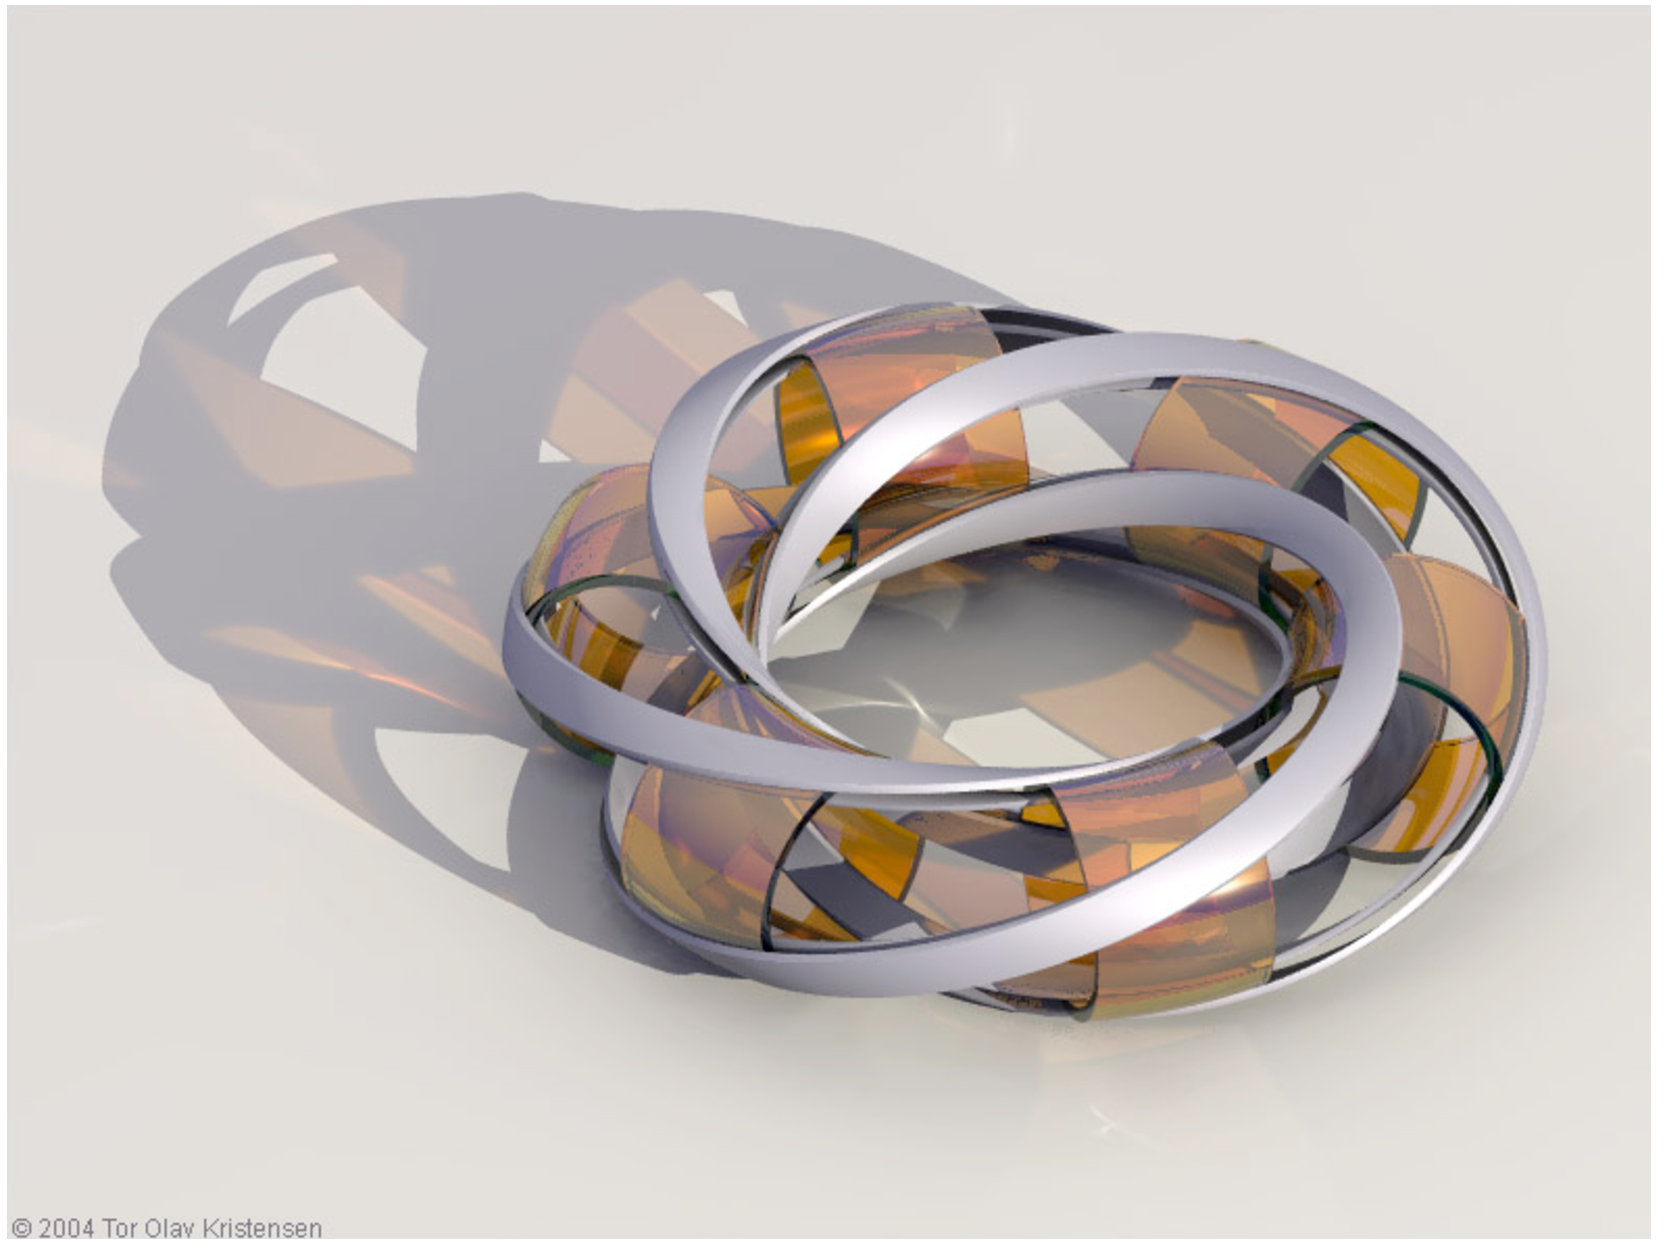
\includegraphics[width=0.485\textwidth]{bilder/pov_ray1}}\quad
\subfigure{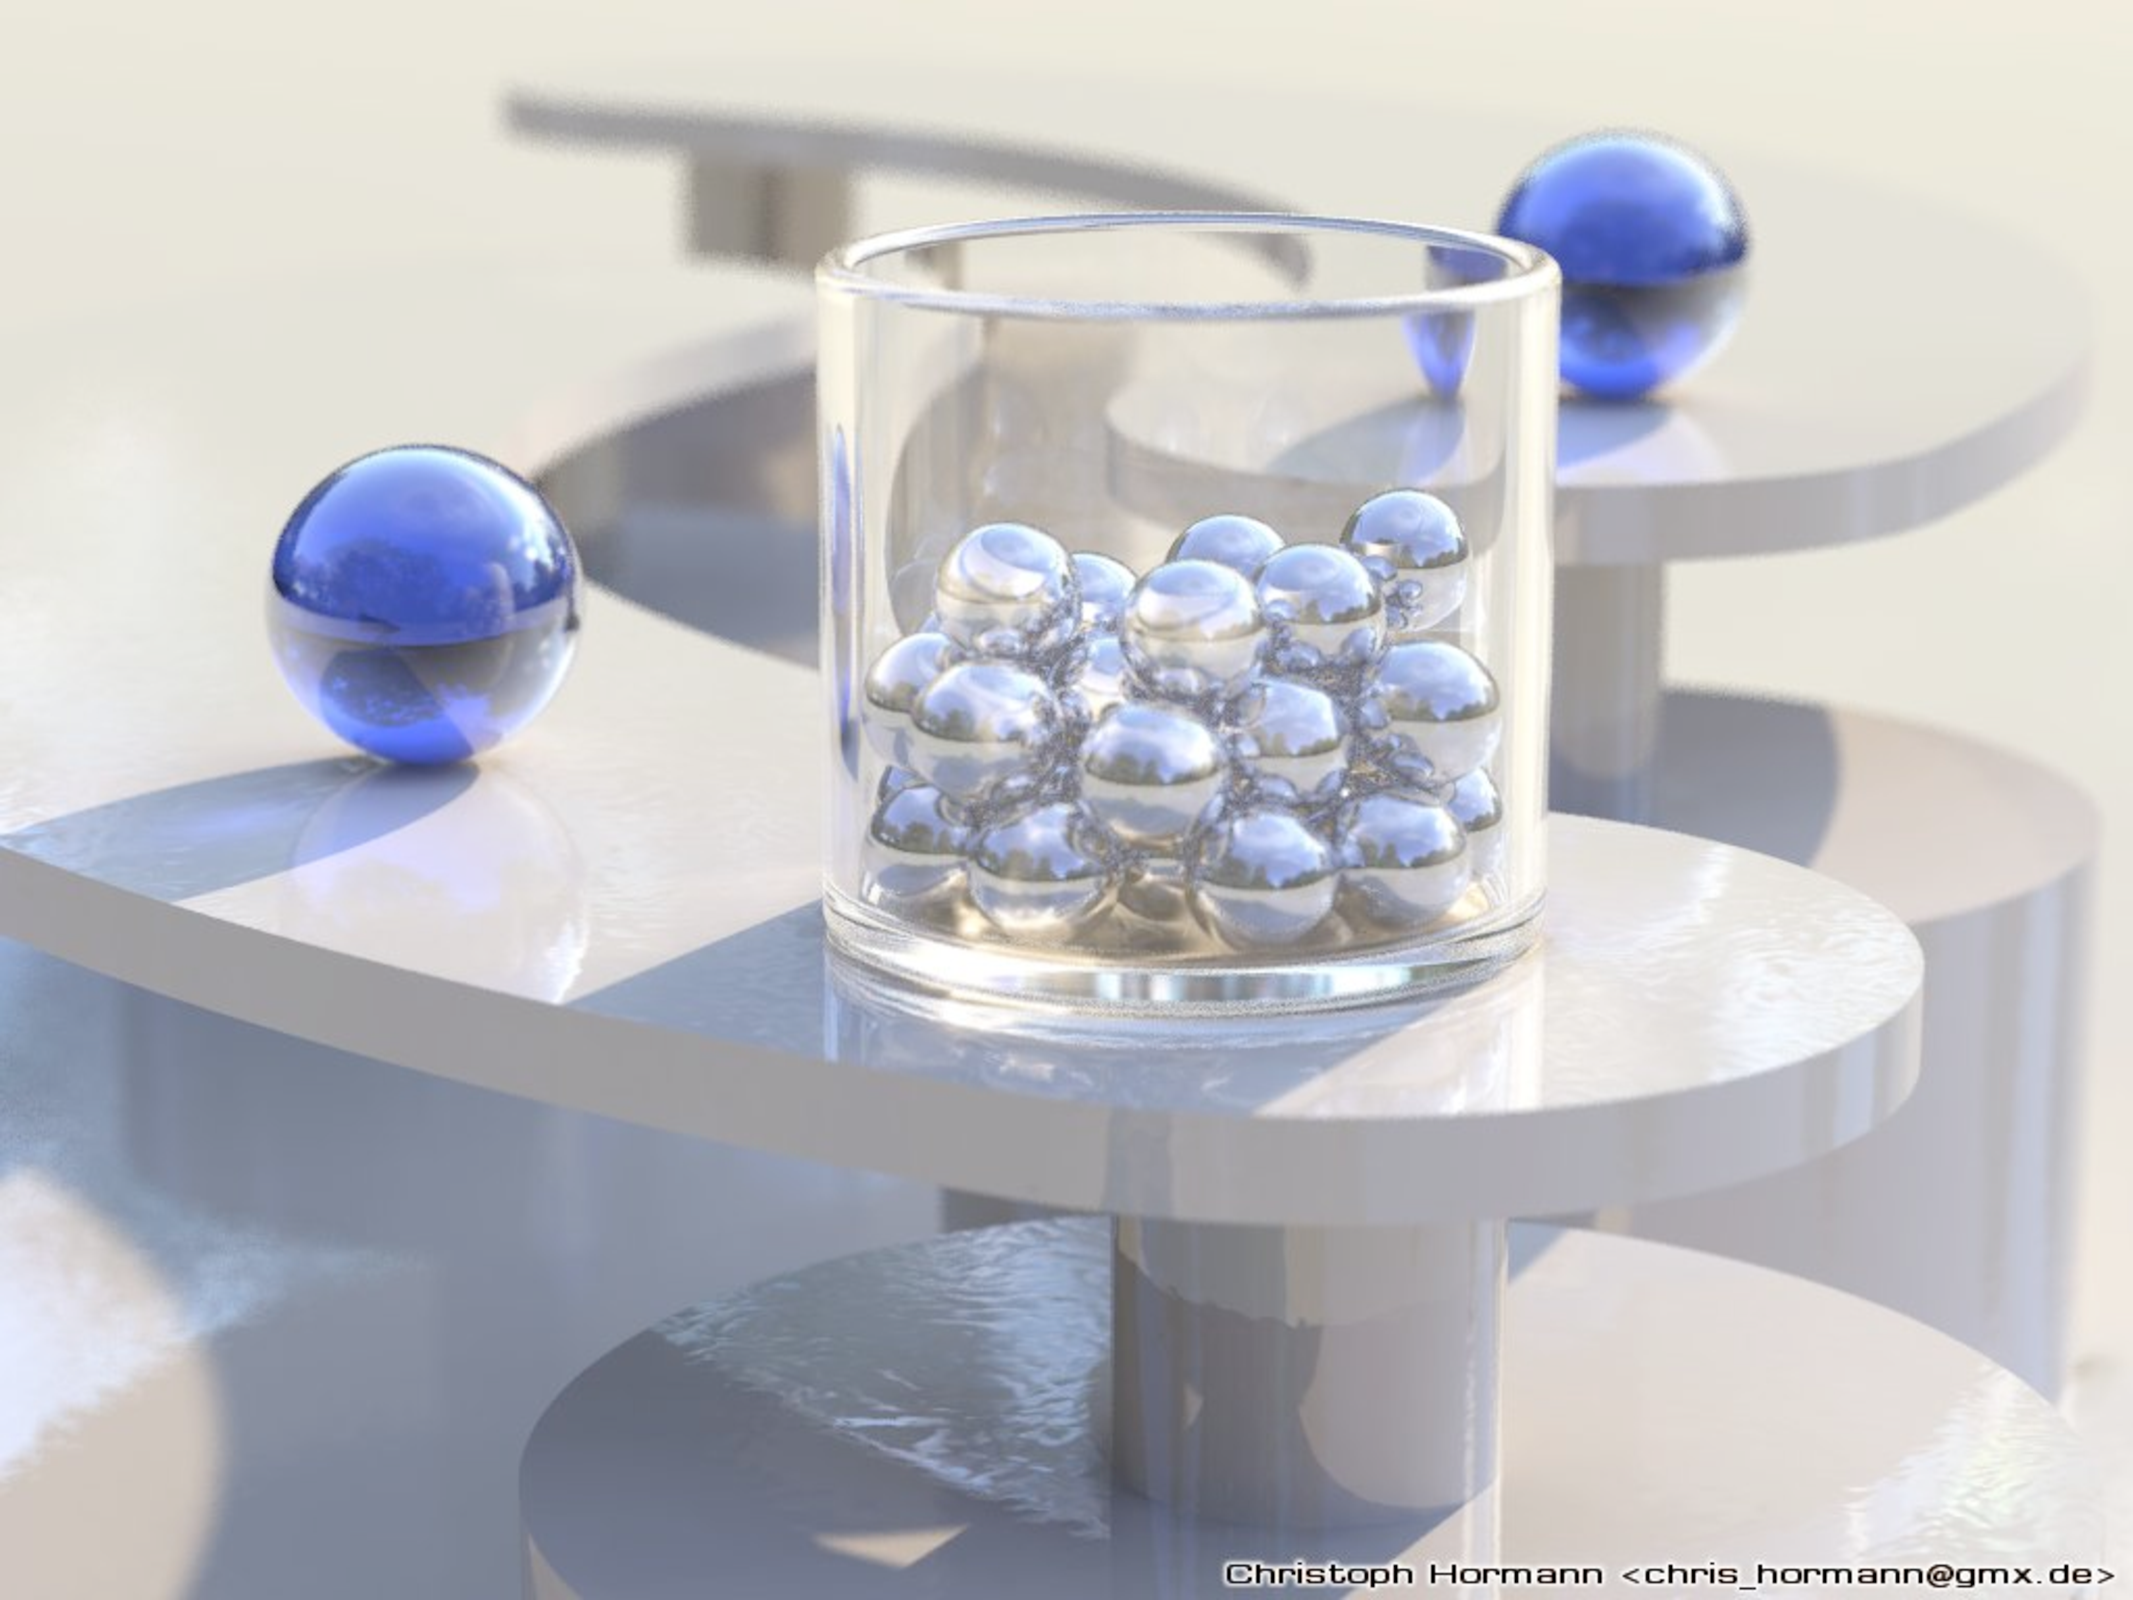
\includegraphics[width=0.485\textwidth]{bilder/pov_ray2}}
\caption{POV-Ray Hall of Fame: Villarceau Circles and Marbles}
\label{fig:halloffame}
\end{figure}

Its worthy to say that with pure ray tracing its not possible to generate these
images. There is always a global illumination model involved that
facilitates the ray tracing algorithm or the combination of these two for
realistic image synthesis.

\subsubsection{Virtual World}
The virtual world in ray tracing is a scene composed of objects and light
sources. This virtual world is viewed thru an virtual eye respectively a
virtual camera. Objects are placed into this virtual world an imaginary
space with height, width and depth that can be seen as a simulation or
imitation of the real world.

Just imagine a real world example, like a pool table and a light hanging
above this table. To imitate such a scene, the scene would consist of a plane
with cut in holes, spheres representing the billiard balls, prisms are modelled
as the boundaries of the table and the queue is an narrowing cylinder. The light
source would be a sphere which looks like a light-bulb. The cameras respectively
the eyes position which represents the viewer is where the scene is viewed from.

Objects in ray tracing are any thing, from solid, to liquid or gas that will be
composed into the virtual world. Not only such simple primitives are objects
in the means of ray tracing. These primitives can be combined to describe even
more complex objects like lamps, cars and so on. ray tracers can only support
objects that can be described mathematically. At first glance it looks like an
big disadvantage but the ability to combine the objects by boolean
operations, this method is called Constructive Solid Geometry (CSG), provides
possibilites to create very complex objects.

To achieve a even more realistic look each object can be patterned with a
texture. A texture is an description of the way how an object looks alike.
Texture attributes can be the color, bumpiness, shininess and an image which
is mapped onto the object to imitate grain of wood, marble and so on.

There is one essential thing in ray tracing, light sources, without light
sources no objects are illuminated hence not seen. Light sources are described
by their position and intensity that describes the color of the light and its
brightness. Modelling the lightning in the virtual world is the catchiest task
in ray tracing \cite{Mosen98}. An image with short-handed light sources will be
swallowed by the darkness and will not show enough detail respectively too
many light sources will flood the image with too much intensity and the
image will loose any shadowing effects.

\subsubsection{Virtual Camera (Eye)}
Two understand the concept of the camera in ray tracing it is important to know
how a pin-hole camera works since it is the simplest and most used model.

A pin-hole camera is simply a light-proof box with a small hole in the front
and a film at the back of the box. The small hole is covered with tape no
light can enter the box. To take a picture the camera is positioned at the
scene and the tape is removed. In order for enough light to enter
the box and strike the film the exposure time of that primitive camera
is higher than in modern, high-tech cameras \cite{Glassner89}.
The aperture has to be small to prevent light saturation of the film. At a time
it allows only a little bit of light into the box. Furthermore it guarantees
that light from a position on the object comes from only one direction and hit
the film in only one position, as shown in figure \ref{fig:pinhole}.\\

\begin{figure}[H]
\centering
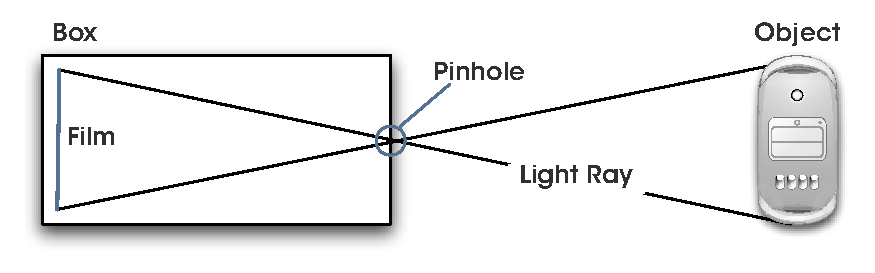
\includegraphics[width=0.6\textwidth]{bilder/pinhole}
\caption{A simple pinhole camera}
\label{fig:pinhole}
\end{figure}


Larger holes, greater aperture size, would lead to blurrier images since light
rays can hit the film in various positions. This effect is also known as focal
blur.

In ray tracing the camera works like a pin-hole camera unlike a real camera the
film is the computer screen the light rays hit. Focal blur is simulated by
shooting a number o sample rays from jittered points to simulate the fact that
light rays can hit the film in variuos positions.

\subsection{Ray Casting}
Ray tracing can be seen as an extension to ray casting. Therefore its easier to
understand ray tracing if the base concept of ray casting are understood. The
next section will introduce ray casting and extend the algorithm to ray tracing.

Ray casting was first introduced by Appel \cite{Appel68} he developed some
techniques for a shading machine for rendering of solids.

First of all it is important to understand the concept of rays. A ray is the
path of a particle of light (photon) extending from the eye into the
scene \cite{Glassner289}. The path is a thin, straight line used to model a beam
of light. Each ray can be seen as a \textit{feeler}\footnote{The ray scans or
rasters the scene that is why a ray is often called a feeler} that reaches the
scene and finds out which objects are visible and what color the object has at a
specific point. Rays are the fundamental element of any ray tracer.

The camera in ray casting and ray tracing can be thought of in many respects to
be kind of pin-hole camera. As shown in figure \ref{fig:pinhole} illustrating the
 pin-hole camera, the film of the camera is now moved out in front of the camera
itself.
The film is referenced as the viewpane or the screen. The pin-hole of the
camera becomes the eye \cite{Glassner89}. The new constellation eye, screen,
object is shown in  figure \ref{fig:eyescrobj}.

\begin{figure}[H]
\centering
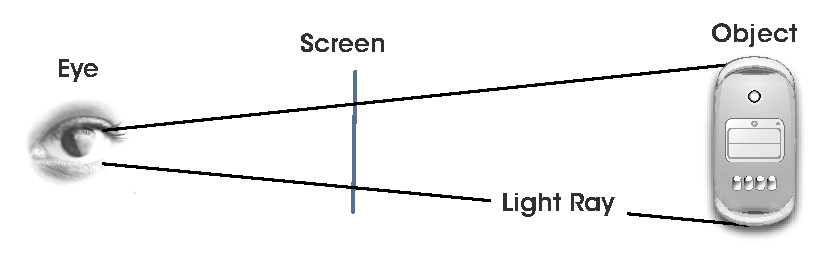
\includegraphics[width=0.6\textwidth]{bilder/eye_screen_object}
\caption{The constellation of the eye, screen and object}
\label{fig:eyescrobj}
\end{figure}


The representation of light on the screen is organized in so called pixels.
A pixel is a point sample not a little geometric square. This misconception
is widespread and it is an issue that strikes right at the root of correct
image computing and the ability to correctly integrate the discrete and the
continuous \cite{AlvyRaySmith95}.

The color of a given pixel is the color of the light that passes from the
object, through the associated pixel into the eye \cite{Hearn94}.

For each pixel on the screen a ray is cast from the eye through the pixel into
the virtual world. Then for each object it is checked if the ray intersects any
of them. If there are several objects in a scene intersected by the ray the
shortest distance to the intersection point is the one that is visible to the
eye. All other intersection are behind the nearest object and not visible
respectively occluded by the visible object. The color at that point is the
accumulated contribution of intensities radiated from all light sources. This
color is given to the pixel through which the ray passed. Ray casting does not
consider light reflected or transmitted by other objects in contrast to ray
tracing.

Ray casters and ray tracers spent most of their time calculating
intersections of rays with different objects. Whitted \cite{Whitted80}
estimates that anywhere from 75 percent to over 95 percent of rendering time
is spent in intersection tests.  For example an image with 640 pixel width  and
480 pixels height, for a total of 307200 pixels, with a medium complex scene
with 100 objects results in 30.720.000 intersection tests. There are well
documented ray tracing accelerating techniques not only to decrease the number
of intersection tests per ray but also to decrease the number of rays, as well
to increase the speed of such intersection calculations.

Ray casting is a simple method to generate images. The major drawback is that
its not possible to generate reflections and refraction. With ray tracing this
drawback has been overcome.

\subsection{Ray Tracing}
The difference between ray casting and ray tracing is that ray casting finds
visible surfaces of the objects whereas ray tracing aditionally determines how
each visible surface looks like. Effects like reflection, refraction, caustics
and shadows are very difficult or even impossible to create with other methods
\cite{Foley90}. But there's a price to pay. Such effects are computationally
very expensive depending on the complexity of the scene and resolution.

The ray tracing Algorithm is defined recursively and was firstly introduced by
\cite{Whitted80}. As beformentioned ray tracing is an extension to ray casting
so the first steps are identical. The ray tracing begins as in ray casting by
shooting a ray from the eye through the screen into the virtual world. The next
step is to find the closest intersection. After determining the intersection
point the raytracer repeats itself by shooting more rays from that point. These
additional rays called secondary rays in contrast to the primary rays are neccessary
 to determine which light sources are directly seen (shadow rays), which objects
 are reflected (reflected rays) and which objects can be seen through the object
 (transmitted rays) at the intersection point.

The secondary rays are treated as primary rays when it comes to trace each of
them. From each ray another set of shadow, reflected and transmitted rays can
be created. Many ray tracers have a recursion depth which actually determines
how often these secondary rays should be generated otherwise the ray count
would increase dramatically and the rendering process would never finish.

The next section will present and explain the three major effects of ray
tracing.

\subsubsection{Shadow}
After the intersection point is determined shadows are calculated by shooting
one ray at each of the light sources contained in the scene. If any opaque
object is between the intersection point and light source than no light via the
ray can arrive at this point hence the point is in shadow. Otherwise if the
light source is not occluded there is a contribution of intensity at the actual
point.

The figure \ref{fig:shadow} illustrates how these shadow rays work.

\begin{figure}[H]
\centering
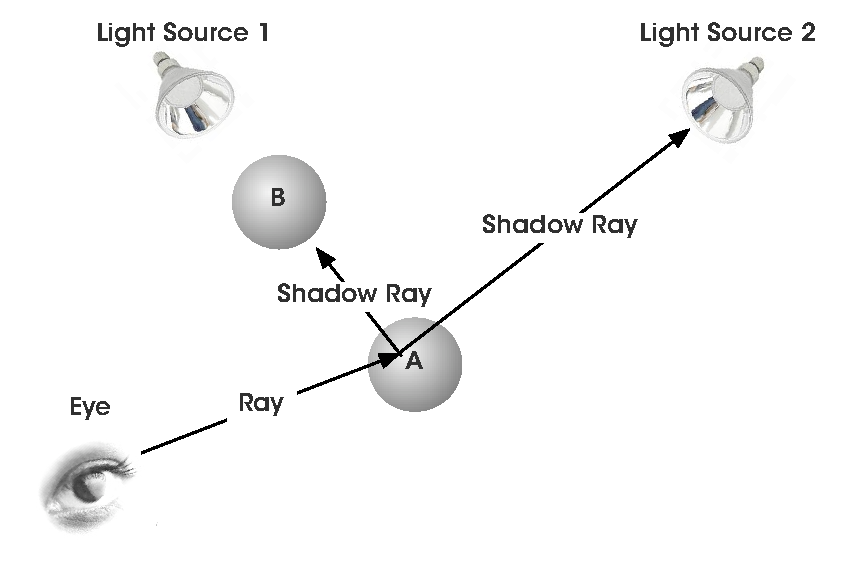
\includegraphics[width=0.6\textwidth]{bilder/shadow}
\caption{How shadow rays work}
\label{fig:shadow}
\end{figure}

The intensity at a specific point are the accumulated intensities of all lights
in the virtual world.

\subsubsection{Reflection}
If the surface is reflective the ray tracer has to determine the color to which
there are contributions of the surface itself and of the color of any reflected
object at that point. Looking in a mirror the object behind can be seen. This is
because the light from those objects travels to the mirror bounces off it and
travels to the eye.

To calculate the reflection the ray tracer needs to calculate the angle at
which the secondary ray should bounce off. By calculating all the
intersecting
objects and finding the nearest one,  determining the surface color at the
point and possibly even reflecting again the resulting color can be carried
back to the pixel through which the original ray was spawned \cite{Hearn94}.

The figure \ref{fig:reflection} illustrates how reflection rays work.

\begin{figure}[H]
\centering
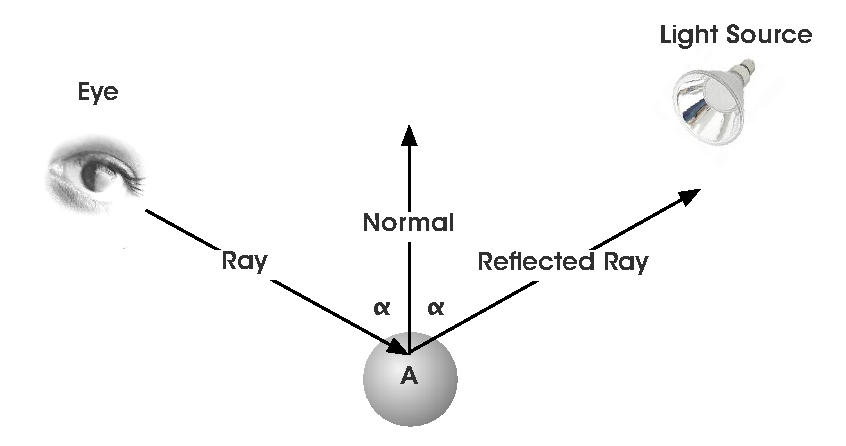
\includegraphics[width=0.6\textwidth]{bilder/reflection}
\caption{How reflection rays work}
\label{fig:reflection}
\end{figure}

\subsubsection{Refraction}
Refraction is modelled similarly to reflection. Instead of bouncing the new ray
of the surface the ray is refracted into the object. Refraction is a optical
phenomenon caused when light travels through one medium to another. Refracting
light is the most commonly seen example, but any type of wave can refract when
it interacts with a medium.

Every object has an index of refraction which describes how fast light travels
through an object as compared to how fast light travels in vacuum. For example
glass has a higher index than water hence the glass will refract the light
stronger than water.

As in the case of reflection the ray can in turn be refracted again or even
reflected. The resulting color is carried back to the pixel through which the
original ray was spawned.

The figure \ref{fig:refraction} illustrates how refraction rays work.

\begin{figure}[H]
\centering
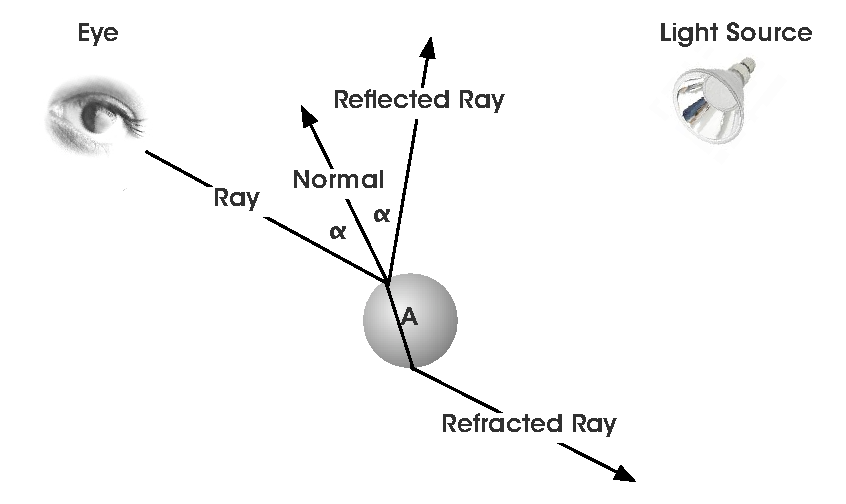
\includegraphics[width=0.6\textwidth]{bilder/refraction}
\caption{How refraction rays work}
\label{fig:refraction}
\end{figure}


\subsubsection*{Pseudo code for the ray tracing algorithm}
The traditional ray tracing algorithm has an recursive character. Without
the evaluation of recursive an reflection rays , without recursion the
algorithm is called ray casting.
\lstset{
        basicstyle=\ttfamily,
        tabsize=8,
        language=Pascal,
        numberstyle=\tiny,
        numbers=right,
        numbersep=5pt,
        stepnumber=1,
        extendedchars=true,
        %frame=lines
	basicstyle=\small
}
\begin{lstlisting}[caption=Ray tracing pseudo code]
for x := 0 to image_width do
begin
	for y := 0 to image_height do
	begin
		raytrace(primary_ray);
	end;
end;

procedure raytrace
begin
	for i := first_object to last_object do
	begin
		find_closest_intersection();
	end;

	for j := first_light to last_light do
	begin
		send_shadow_ray();
	end;

	shade_pixel();

	if coeff > 0.0
	then
		raytrace(reflected_ray);
		raytrace(refracted_ray);
	end;

	return color;
end;

\end{lstlisting}

There are two terms that are used in ray tracing to describe the art of a ray
tracer. First of all there is the term \textit{backward ray tracing}, the
standard ray tracing algorithm follows the path of light from the eye backward
to the light source. In that sense it is referred as backward ray tracing.
Approaches that follow casting rays the other way from light sources to the
viewer are referred as forward ray tracing \cite{Foley90}.

The ray tracing algorithm has some limitations that the global illumi\-nation
alternatives like Radiosity and Photon Mapping try to conquer.

Global illuminaition models are critical in generating realistic looking
images. The results are comparable to images taken from the real world.
Global illumination in general environments is a complex task. Global
illumination models are designed to approximate the rendering equation \cite
{Kajiya86} which describes the complete transport of light bouncing in the
virtual world.

\subsubsection*{Radiosity}
Radiosity \cite{Shirley00} is a finite element method that computes a view
independent global illumination solution as a finite mesh. The environment is
divided up into patches that are uniform and perfectly diffuse. Energy is
transferred between these patches until an equilibrium is established.
Radiosity couples the lightning information to the geometry. If the geometry
changes the Radiosity process has to be repeated until a new equilibrium is
established. Furthermore this tight coupling of geometry and light is costly to
calculate and meshing artifacts can occur if not carefully constructed.
Currently most Radiosity implementations combine ray tracing and Radiosity
\cite{ProMulltGI91} \cite{Shirley90} \cite{ZimmerShirley95} because Radiosity
doesn't handle arbitrary reflection models. Even though ray tracing has been
extended with Monte Carlo Techniques and Radiosity has been extended with
directional capabilities neither of the two methods precludes the use of the
other.

On the one hand ray tracing combined with Radiosity can produce very realistic
looking images. On the other hand ray tracing with Monte Carlo Techniques is
very time consuming and can produce noisy results while Radiosity uses a lot of
memory to store the information needed and as said before can not handle
specular reflection properly.

\subsubsection*{Photon Mapping}
Another global illumination method is Photon Mapping developed by Henrik Jensen
\cite{Henrik96}. Photon Mapping is a two pass global illumination algorithm
that overcomes the disadvantages of Monte Carlo ray tracing techniques. Photon
mapping decouples the lightning information from the geometry as an opposite to
Radiosity. The information is stored in a spatial data structure called the
photon map. For caustics \cite{Wiki06} \footnote{A caustic is the envelope of
light rays
reflected or refracted by a curved surface or object, or the projection of that
envelope of rays on another surface - wikipedia.com} another map is used and
seperately handled. The figure \ref{fig:caustics} shows caustics which appear
with transparent objects and can be generated with photon mapping.

This decoupling allows Photon Mapping to calculate the rendering equations terms
seperately and store them in different photon maps e.g. in the befromentioned  caustics map. This makes Photon Mapping a very flexible and powerful algorithm,
since each term of the rendering equation can be solved using other techniques.
Furthermore photon mapping has been extended to handle sub-surface scattering
and volume caustics.

\begin{figure}[H]
\centering
\subfigure{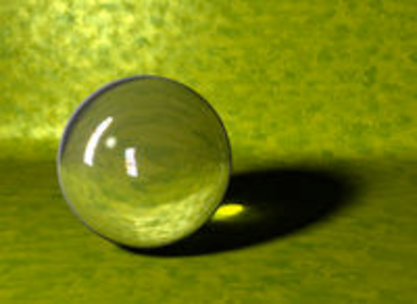
\includegraphics[width=0.323\textwidth]{bilder/200px_caustics}}\quad
\subfigure{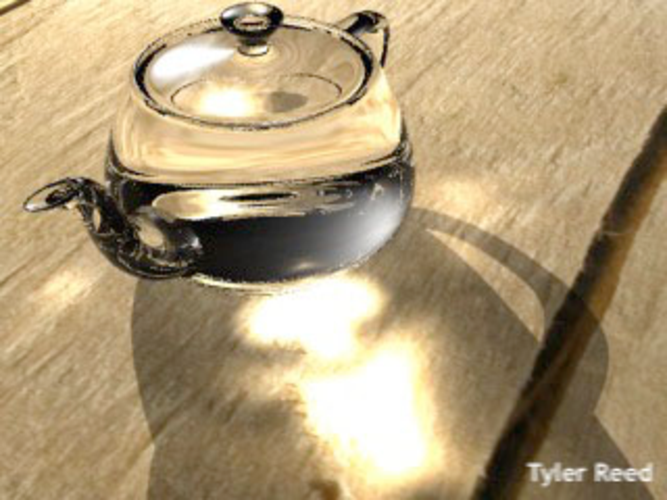
\includegraphics[width=0.313\textwidth]{bilder/brazil_caustics}}\quad
\subfigure{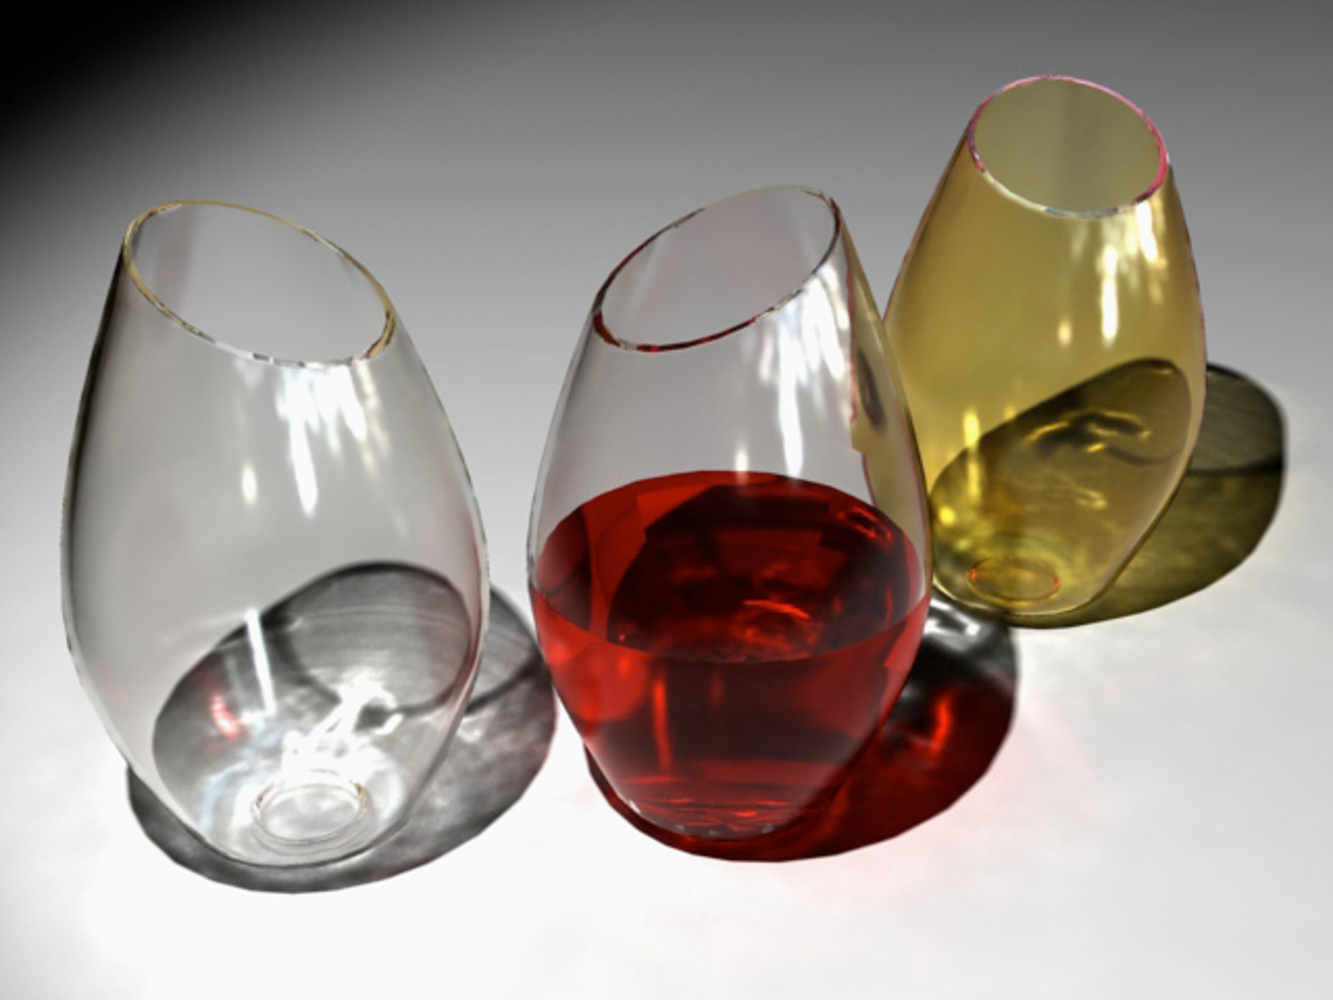
\includegraphics[width=0.313\textwidth]{bilder/caustics}}
\caption{Caustics which appear with transparent objects}
\label{fig:caustics}
\end{figure}

\newpage
\section{Cell Broadband Engine}
The Cell Broadband Engine is the result of a collaboration between Sony, Toshiba
and IBM. The Cell BE is the first microprocessor of a new family which confirm
to the Cell Broadband Engine Architecture. The Cell BE extends the 64-bit
PowerPC Architecture \cite{IBMhb06}.

\begin{figure}[H]
\centering
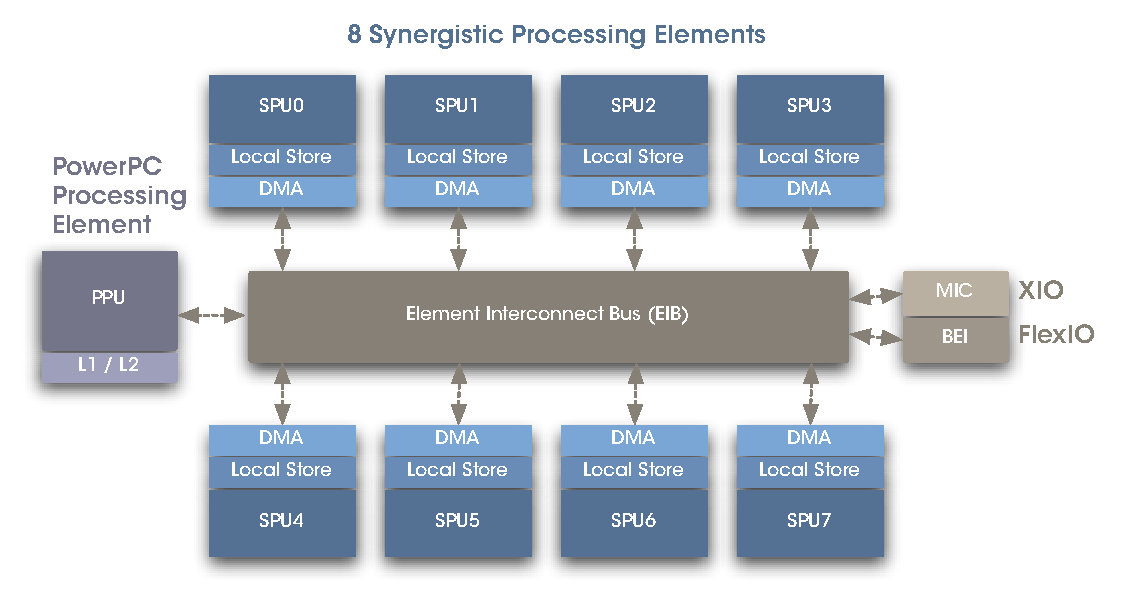
\includegraphics[width=\textwidth]{diagramme/cbe}
\caption{Architectural Overview of the Cell Broadband Engine}
\label{fig:cbe}
\end{figure}


Figure \ref{fig:cbe} shows a high-level view of the first implementation of Cell
BE. It includes a general-purpose 64-bit POWER Processing Element (PPE). In
addition, the Cell BE incorporates eight Synergistic Processing Elements (SPEs)
interconnected by a high-speed, memory-coherent Element Interconnect Bus (EIB).
This initial implementation of Cell BE is targeted to run at 3.2GHz.

The SIMD units on the eight SPEs provide the majority of the computational power
of the Cell BE. When using single-precision floating-point fused multiply-add
instructions, the eight SPEs in the first-generation Cell BE chip can perform a
total of 64 floating-point operations per cycle.

The integrated memory controller (MIC) provides a peak bandwidth of 25.6GB/s to
an external XDR memory, while the integrated I/O controller provides peak
bandwidths of 25GB/s (for inbound) and 35GB/s (for outbound). The EIB supports a
peak bandwidth of 204.8GB/s for intra-chip data transfers among the PPE, the
SPEs, and the memory and the I/O interface controllers \cite{IBMhp05}.


\begin{description}
\item[\color{Bigblue}{PowerPC Processor Element (PPE)}]
The PPE consists of a POWER Processing Unit (PPU) connected to a 512KB L2 cache.
The PPE is the main processor of the Cell BE, and is responsible for running the
operating system and coordinating the SPEs. The key design goals of the PPE are
to maximize the performance/power ratio as well as the performance/area ratio.
The PPU is a dual-issue, in-order processor with dual-thread
support.

The PPE core can fetch four instructions at a time, and issue two. In order to
improve performance from its in-order pipeline, the PPE utilizes
delayed-execution pipelines and allows limited out-of-order execution of load
instructions. This allows the PPE to get some of the advantages of out-of-order
execution without any significant increase in complexity. We do not focus on the
PPE in this paper since most of the algorithms presented here do not utilize the
PPE.\cite{IBMhp05}.



\item[\color{Bigblue}{Synergistic Processor Elements (SPEs)}]
 The SPE is a modular design consisting of a Synergistic Processing Unit (SPU)
and a Memory Flow Controller (MFC). An SPU is a compute engine with SIMD support
and 256KB of dedicated local storage. The MFC contains a DMA controller with an
associated MMU, as well as an Atomic Unit to handle synchronization operations
with other SPUs and the PPU.

An SPU is a dual-issue, in-order machine with a large 128-entry, 128-bit
register file used for both floating-point and integer operations. The SPU
operates directly on instructions and data from its dedicated local store, and
relies on a channel interface to access the main memory and other local stores.
The channel interface, which is in the MFC, runs independently of the SPU and is
capable of translating addresses and doing DMA transfers while the SPU continues
with the program execution.

The SPUs SIMD support can perform operations on sixteen 8-bit integers, eight
16-bit integers, four 32-bit integers, or four single-precision floating-point
numbers per cycle. At 3.2GHz, each SPU is capable of performing up to 51.2
billion 8-bit integer operations or 25.6GFLOPs in single precision.

Features such as a deterministic local store access time, simple issue rules,
software-inserted branch hints, a large register file, and so on, are exposed to
the compiler and applications for performance tuning. With some tuning efforts,
we have seen a wide variety of applications approach the theoretical
instructions per cycle (IPC) of 2 in
the SPU. The SPEs have DMA support for excellent data streaming bandwidth that
is much higher than many modern processors \cite{IBMhp05}.

\item[\color{Bigblue}{Element Interconnect Bus (EIB)}]
The PPE and SPEs communicate coherently with each other and with main storage
and I/O through the EIB. The EIB is a 4-ring structure (two clock-wise and
two counterclockwise) for data, and a tree structure for commands. The EIBs
internal bandwidth is 96 bytes per cycle, and it can support more than 100
outstanding Direct Memory Access (DMA) memory requests between main storage and the SPEs
\cite{IBMhb06}.
\end{description}

\subsection{Programming Overview}

The SPEs are optimized to run computational tasks and only the PowerPC core is
able to run a generic operating system or a kernel. The kernel is
the only software that can directly interact, communicate with the
SPEs. The kernel has to abstract the hardware interface into a mechanism that
allows applications in userspace access to the SPEs since the access to the
controlling registers is only possible in the privileged mode.

Its worthy to say that GNU/Linux is the only operating system running
currently on Cell. The porting of the Linux kernel was not challenging as
someone would guess, as the Linux kernel has capabilities of running on PowerPC
G3, G4 the PowerPC 970. Therefore for the next considerations a GNU/Linux is
assumed.

Several ideas have come up for an abstraction mechanism. The abstraction
mechnism had to provide some functionality that allows the loading of a program
into a SPE, synchronizing the execution and transferring memory between
an SPE program and a host system. From a developer point of view it was also
important to have such tools like gdb and oprofile available.

The final abstraction mechanism was a virtual file system the SPU file system.

A virtual file system provides a defined interface between the kernel and to a
concrete system. In Linux exists several such virtual file systems. As an
example the \textit{procfs} provides information about processes, hardware and
the information can be retrieved with open, write and read system calls.

The spufs maps hardware resources into specific files which reside in a
directory structure that refer to a logical SPE context. For example the
\textit{mem} file represents the local store memory of the SPE and any process
can open the file and open, read and write to the file. Further files are
\textit{run} which starts the execution of the SPE when written to it and the
three files \textit{mbox, ibox, wbox} which abstract the mailbox facility of
each SPE.

Further abstraction accommodated a library interface that is thread-oriented
and behaves similary to the pthread library. As an addition to the library
compiler and binutils were made available since the SPEs instruction set is
different to existing CPU architectures. The whole toolchain, patches to the
kernel, debugger and abstraction library were made available for download
\cite{Bsc06}.

The knowledge of the \textit{spufs} facilitates the developer to write code
at a higher abstraction layer so reusability and maintainability is preserved.

\subsubsection{General Programming Workflow}
There are two ways of programming applications for the Cell. One is the use of
remote procedure calls and the other with the SPU file system.

The remote procedure (RPC) call will be not fully explained, just a brief description will be given, it is only mentioned for the sake of completness. The RPC mechanism allows the PPE to call a SPE function as it were a regular function call. As the RPC mechanism known in other environments this facility includes an Interface Description Language (IDL), its compiler and the IDL runtime library too \cite{STI05}.

The second way is the use of the \textit{spufs}\footnote{SPU File System} and
the PPE abstraction library. The general workflow of porting an application to
the Cell Broadband Engine is illustrated by the following listing:
\subsubsection*{General Workflow of Porting to CBE}
\begin{description}
\item [\color{Bigblue}{\color{Bigblue}{$\triangleright$}}] Porting to the PPE
\item [\color{Bigblue}{\color{Bigblue}{$\triangleright$}}] Application partitioning
\item [\color{Bigblue}{\color{Bigblue}{$\triangleright$}}] Offloading parts to the SPEs
\item [\color{Bigblue}{\color{Bigblue}{$\triangleright$}}] Using SPU C/C++ language extensions to achieve maximum performance
\item [\color{Bigblue}{\color{Bigblue}{$\triangleright$}}] Tuning data access and flow with double-buffering and
prefetching
\item [\color{Bigblue}{\color{Bigblue}{$\triangleright$}}] SIMD vectorization
\end{description}

\subsubsection*{I. Porting to the PowerPC Processing Element}
As a first step the target application has to be ported to the PPE. Often is
it only needed to recompile the application. Caution is advised with low level
functions that operate on bits. It has to be remembered that the PPE is based
upon a 64-bit PowerPC and hence the byte ordering is Big Endian in contrast to
x86 based processors (Intel/AMD) which have Little Endian byte ordering.

\subsubsection*{II. Application Partitioning}
This is an essential step in the progress of porting to Cell. The developer
has to decide which parts or calculations should be done on the SPEs.
Parts with heavy computation and code which can be vectorized should be offloaded
 to the SPEs since there are the \textit{work horses} of the Cell. This process
can be done manually or by the compiler. In this case the developer pastes hints
 to the compiler which parts should be offloaded.

\subsubsection*{III. Offloading Parts to the Synergetic Processing Elements}
After identifying the parts to be offloaded the environment from the SPE point
of view has to be setup. The developer has to provide functions to the SPE that
allocate essential data structures, fetch the needed data into the local store
and save the computational results back to main memory. Furthermore if its not
possible to feed the SPE with work in a simple way a scheduler respectively a
load balancer has to be implemented.

\subsubsection*{IV. Using SPU C/C++ Language Extensions}
The initial code offloaded to the SPEs is not optimized for vector units. To achieve a
higher performance the heavy computational parts should be rewritten with the
SPU C/C++ language extensions to achieve maximum performance. They provide
Intrisics \footnote{Intrinsics are assembly-coded functions that enable the
programmer to use C/C++ function calls and variables in place of assembly
mnemonics and registers} for Byte Operations, like mask, logical, shift and
rotate intrinsics, special intrinsics for Memory Flow Controller (MFC) Input and
 Output and a whole bunch of intrinsics for manipulating vector data types \cite{IBMle06}.

\subsubsection*{V. Tuning Data Access and Flow with Double Buffering and
Prefetching}
The access to main memory from the SPE in a sequentiell manner is not a good idea.
 The Cell is capable of DMA hence it is a good idea to use double buffering for
higher performance. The idea behind double buffering is to have two or more buffers.
 On the one buffer the computation is performed and the other buffer is
simultaneously filled with the needed data. When the computation of the first
buffer is done the buffers are swapped. Double buffering is not a new technique
it is often used and common in the field of computer graphics.

If it is predictable which data is needed another technique to minimize the wait
for DMA completion is the use of prefetching. Data which is in the near future
needed should be prefetched so that the computational part need not wait.


\subsubsection*{VI. SIMD Vectorization}
As a last step of optimizing the code to Cell is the use of
SIMD\footnote{Single Instruction Multiple Data} vectorization. The native data type
of the SPEs are vectors. The loading and storing of registers is all done in the
size of an vector. Therefore it is recommended to port the scalar code fully to SIMD
 code. There is a significant overhead on operations with scalar values which should
 not be discarded.

The SPE performs best with SIMD code and with the use of SPE C/C++ intrinsics.
The SPEs are SIMD-only processor with no hardware branch prediction,
instruction issue restrictions and single ported memory.

\section{State of the Art}
Nowadays the major role of rendering images on a computer play rasterization
algorithms. Virtual reality applications as well games are rendered on hardware which
 is based on rasterization algorithms. Furthermore interactive rendering is almost
 exclusively the domain of these algorithms but they have major drawbacks which have
 to be considered in the of manner of interactive rendering. Rasterization algorithms
as well as raterization hardware lack of support for parallel processing and realism. It is very difficult
 to scale the graphics pipeline efficiently which is essential for parallel computing.
 Further issues are the communication requirements between parallel units, and the
 need to avoid redundant processing and data storage as for textures \cite{Eldrigde00}.

As mentioned before another big issue is the weakness to realism. Eventhough the
rasterization algorithms have been extended with many features for shading it
is very difficult for developers to express some optical
phenomena\footnote{Optical phenomena like caustics, color bleeding} in code, despite
of the rasterization algorithm used.

Ray tracing has some superior features over rasterization based
algorithms that would make it a interesting alternative for generating computer
synthesized images \cite{Wald101}.\\\\
Short summary of advantages and disadvantages of ray tracing:
\subsubsection*{Advantages}
\begin{description}
\item[\color{Bigblue}{$\triangleright$}] Calculation of shadows from multiple lights,
reflections refraction and correctly calculated in dynamic scenes without using
static fakes like environment mapping
\item[\color{Bigblue}{$\triangleright$}] Line, area and volume lights with correct shadow casting
\item[\color{Bigblue}{$\triangleright$}] Usage of procedural textures with almost infinite
accuracy
\item[\color{Bigblue}{$\triangleright$}] Volumetric lightspaces with real 3-dimensions
\item[\color{Bigblue}{$\triangleright$}] Materials can be modelled via arbitrary illumination
modells and layered material textures.
\item[\color{Bigblue}{$\triangleright$}] Curved objects without using splines
\item[\color{Bigblue}{$\triangleright$}] Realtime boolean algebra operations in dynamic scenes
like intersection, semi-intersection and exclusion
\item[\color{Bigblue}{$\triangleright$}] Higher image quality with anti aliasing and depth of
field
\item[\color{Bigblue}{$\triangleright$}] No usage of special hardware
\end{description}
\subsubsection*{Disadvantages}
\begin{description}
\item[\color{Bigblue}{$\triangleright$}] Complex mathematic algorithms hence long
implementations time
\item[\color{Bigblue}{$\triangleright$}] Almost 100\% of calculations done by the CPU contrary
to rasterization which is done almost of all calculations on GPU
\item[\color{Bigblue}{$\triangleright$}] Scene modelling done via specialized editors
with various export filters
\item[\color{Bigblue}{$\triangleright$}] Large amounts of memory needed for detailed scenes and the results
\end{description}


\subsection{Interactive Ray Tracing}
Ray tracing base become a possible alternative to the current rasterization for
interactive 3D graphics. In the past many contributions to ray tracing
acceleration and recent special purpose Hardware like the SaarCOR chip made Ray
Tracing to some point competitive to the rasterization algorithms.
The availability of these prototype graphics boards purely based on ray tracing
and the knowledge of new algorithms could have significant consquences for
computer gaming Considering the advantages of ray tracing there is very few
information available how computer games could benefit from ray tracing
\cite{Schmittler04}.

There have been or still exist two approaches to adapt ray tracing
to games. First of all there is the ray tracing Engine for the well-known Ego
Shoooter Quake 3 Arena. The efforts were concentrated on adapting shading
effects an general game managment, things like reflection refraction and
shadows were not taken into account cause the ray tracing provides such
effects. All effects which provided the traditional effects engine could be
rendered with ray tracing while most effects were significantly simpler to
implement.


The second game called "Oasen" featured a ray tracing only game engine. The
game was from ground up designed to use ray tracing as the backend for
rendering. The rendering engine featured effects like moving sky, changing
light situation, day time simulation and many more. The ray tracing engine was
also used for collision detection, physics engine and
acoustics hence many complex and special algorithms were avoided
for those tasks \cite{Schmittler04}.

The feature richness has there price. The system requirements for frames
with 640x480 pixels resolution are huge. A cluster of PC's forming a virtual
CPU with 30 GHz are required to render the images \cite{Schmittler04}.

Furthermore there is a demo available from Realstorm Ray
Tracing\footnote{http://www.realstorm.com/} which is a bowling game also
completely rendered with ray tracing.

The only available ray tracing framework is the OpenRT project of the
Universit\"ät Saarbr\"ucken. The main point of the project is to develop ray
tracing to the point where it offers an alternative to the current
rasterization based approached for interactive 3D graphics. The project consist
of an realtime ray tracing core and OpenRT-API like OpenGL, SDL and Mesa and a
whole bunch of applications for simulation, animation, global illumination and
prototype visualization.

As an addition to the ray tracing approaches for games and the framework there
exist many other projects which deal with interactive ray tracing. These
projects are not applied to any games there are just pure ray tracer and show
the progress and possibilites of ray tracing \cite{Wald04} \cite{Wds04}
\cite{Wbs03} \cite{Bws03} \cite{Gws04}.

The feature richness of ray tracing to generate high quality images with highly
accurate optical effects makes it an interesting technology for future computer
games \cite{Schmittler04}.


\subsection{Ray Tracing Hardware}
Graphics hardware based on the ray tracing algorithm is very rare. Currently
there are two existing implementations of ray tracing hardware. First of all
there is the Advanced Rendering Technologies VPS\footnote{http://www.artvps.com/}
company that sells ray tracing hardware for offline rendering\footnote{Performance
is only of second priority with offline rendering contrary to real-time rendering}.
Secondly there is the Saarland University that develops a real time
ray tracing chip. They have published two designs the SaarCOR
\footnote{http://www.openrt.de/} and the Ray Processing Unit (RPU).

The AR350 is a ray tracing processor developed by Advanced Rendering
Technologies VPS company. By using an array of AR350 processors, the PURE and
RenderDrive products achieve high performances in ray tracing based rendering.
The capabilities of the processor are global illumination computation by
implementing Path Tracing based methods and an RenderMan \footnote{RenderMan is
an umbrella term which is often used to refer to the RenderMan Interface
Specification, RenderMan Shading Language and the Photorealistic RenderMan
Interface} compliant interface \cite{Cassagnabere05}.

The SaarCOR is also a ray tracing chip developed by the Saarland University.
The RT-Chip achieves the same graphics performance as rasterization hardware.
Furthermore the RT-Chip is much simpler than actual rasterization hardware.
An additional advantege of the RT-Chip is reduced usage of external memory
and therefore it is lesser limited than actual graphics technologie.

The limitation of rasterization hardware is caused due to the high need of
memory bandwith. Frequent overwrites of pixels in the framebuffer \footnote{The
framebuffer is such an external memory} and its heavy use of the Z-buffer
and stencil-buffer requires the latest memory technology and high memory
clock rates to reach the needed performance.

This is an important fact considering to bring the ray tracing algorithm on
programmable Graphics Hardware. There have been several approaches of porting
ray tracing on the GPU \cite{Purcell03} \cite{Christen05}. The first
showed that ray casting \footnote{For more information see section ray casting}
can be done efficiently in graphics hardware unfortunately ray casting
doesn't allow the generation of high quality images. The second implementation
was a full featured ray tracer with reflection and refraction but lacked of
support for global illumination an texture support.

To summarize ray tracing hardware is possible and exists but is rare. Ray
Tracing on GPU's is limited due to memory size concerns which
disallows rendering of high resolution images with a lot of textures.

\section{Related Work, Previous Results}
The use of ray tracing for interactive applications is relatively new. Recent
demonstrations \cite{Parker99} showed the capability of ray tracing for
interactive rendering. This full featured ray tracer including parametric surfaces
and volume objects could achieve high frame rates on a large shared
memory supercomputer. The implementation \cite{Parker199} \cite{Parker299} was
optimized for cache performance and parallel execution.

They showed that ray tracing scales well with increasing numbers of processors.
Even a scene with thousands of primitives could be rendered at high frame rates.

Furthermore Pharr et al. \cite{Pharr97} showed that coherence can be exploited
by reordering the rendering computation. They were able to render scenes with
up to 46 million triangles but their system was far from real time
\cite{Wald01}.

\subsection{Previous Results}
Effort was also invested into an implementation of ray tracing on a CBE
\cite{Pablo05}.The implementation was done within the scope of a master
thesis at the IBM lab. It is referred to in the following as the
\textit{predecessor work}.
The \textit{predecessor work} for the Cell Broadband Engine was based upon a pipeline
programming model. Each SPE contributed an specific amount of work during the
whole ray tracing process. The first phase of the rendering pipeline was the
generation of primary rays. The second phase included the traversal through the
grid and the intersection of rays with the objects. The third phase was
responsible for shading the actual pixel at the intersection point.

The space partitioning and the assignement of each object to a specific
voxel\footnote{A voxel is an abbreviation of volume element and pixel = voxel}
was done on the PPE.

\subsubsection*{Summary of tests with the old Cell ray tracer}
To get an first impression of the complexity and data flow of the ray tracing
algorithm several tests were executed with the old Cell ray tracer as a base.


It turned out that an important part of the ray tracing process was split
apart and offloaded to two different SPEs. This circumstance led to a
situation where computation was performed twice. Furthermore each computation
depended on the rays of the other SPE and the rays were copied from one SPE
to the other and back.

The following table shows how many rays are propagated back for traversal and
reapplication of intersection tests due to the unawareness of the actual
intersection point.

\begin{table}[h]
\centering
\begin{tabular}{|c|c|c|c|c|}
\hline
\textbf{\textsf{{Resolution}}} &
\textbf{\textsf{\textbf{Rays in total}}} &
\textbf{\textsf{\textbf{Rays with hit}}} &
\textbf{\textsf{\textbf{Rays reprocessed.}}} &
\textbf{\textsf{r\textbf{Percentage}}}\\
\hline
64x64 & 4096 & 1556 & 1011 & ~64.7 \%\\ \hline
256x256 & 65536 & 34984 & 17923 & ~51 \%\\ \hline
2400x2400 & 5760000 & 2685992 & 2322923 & ~86.4 \% \\ \hline
\end{tabular}
\caption{A comparison of rays with hit and rays which are reprocessed}
\end{table}

As the above table shows, a big number of rays had to be processed again.
Additionally to the computation overhead produced due to the
partitioning of the algorithm an significant amount of
overhead came along because the rays had to be written and read from the main
memory. A big gain of time (about 32\%) was achieved after joining the two
spulets.\\\\
\textbf{Testcase\footnote{Tests were performed with a resolution of 1200x1200
pixel, an object complexity of 8 and recursion depth of null} 1: Original
time: 77.36 sec New time: 52.73 sec}\\

A further improvement was the SIMDizing of the intersection tests. The big
advantage of SIMD is the facility to compute 4 values simultaneously with only
one instruction.
Geometric versions of intersection tesst work with vector arithmetic and are
predestinated for SIMD-Code. Instead of sequentially computing each coordinate
this is done with only one instruction. In addition the overhead of rotating
and placing variables into the registers is eliminated\footnote{The
SPU's are vector units and the only data type which there are aware of is a
vector. All other data types are converted into a vector, calculated and
stored and afterwards casted back to the original data type}.
Tests showed that an big amount of instructions were eliminated and
another gain of time was recorded.\\\\
\textbf{Testcase 2: Original time: 77.36 sec New time: 43.68 sec}\\

Another crucial point was the access to the main memory. In many places objects
like light sources and primitives were fetched sequentially and object by object.
A combination of several objects into a list could improve the performance
further. Targeted branch hints gained about 1\-2 seconds lesser
computational time too.\\\\
\textbf{Testcase 3: Original time: 77.36 sec New time: 35.42 sec}\\
After all these tests a new computational time was achieved, which was two times
faster than the original time. These tests and considerations were taken into
account for the new application architecture.



\chapter{System Analysis}
For the new hardware architecture Cell Broadband Engine a ray tracing
application architecture will be implemented. The Cell BE offers superior
computational features that makes it a preferred candidate for ray tracing.
Existing application-specific integrated circuits (ASIC) are just prototypes
and not available to the end user.

Since ray tracing is becoming more and more important for
real time rendering existing hardware should be investigated for capabilities
for interactive content.

This work wil present a solution for a ray tracer that will render frames at
acceptable rates. Furthermore this work will show that interactive ray tracing
is possible with general purpose hardware like the Cell BE and is not dependend
on special ray tracing hardware.

Therefore several approaches for ray tracing architectures will be introduced
and will be examined with respect to their performance and their capabilities
for ray tracing.

\section{Requirements Specification}
The requirements are the result of a preliminary examination of the hardware
and existing software. The first step included to get familiar with the
hardware and to understand how the Cell BE works. There are many things
which have to be considered when developing for the Cell BE. Hardware constraints
as well as architectural features are taken into account when specifiying the
requirements.

Beside the hardware the analytical analysis of the \textit{predecessor work} for the Cell BE yield to software constraints that are as well taken into account.

The hardware and software constraints were the major points which influenced the
 requirements for load balancing, caching and the programming model.


\subsection{The Purpose of the Project}
\paragraph{RQ10000:} The new application architecture should make it possible to
render realistic images in real time. The necessary rendering algorithm has to be ray tracing.

\subsection{Top-Level Requirement}
\paragraph{RQ10001:} For the new hardware architecture the Cell Broadband Engine a
ray tracer has to be implemented. The ray tracer itself shall be based on the
classical algorithm developed by Turner Whitted. For maximum performance the
application architecture has to be adapted to the hardware and has to take
advantage of its many computational features.

\subsection{Mandated Constraints}
\paragraph{RQ10010:} It is recommended that most computational workload is to be done
on the Synergetic Processing Elements.
\paragraph{RQ10020:} All work where a branch prediction is needed should be done on
the PPE.
\paragraph{RQ10030:} The creation and deletion of the main data structures should be
done on
the PPE. The PPE has unrestricted access to main memory.
\paragraph{RQ10040:} It is
recommended to develop an efficient cache management. The Synergetic Processing
Element have no hardware cache.
\paragraph{RQ10050:} The Synergetic Processing Elements are
optimized for single precision calculations. It is recommended to avoid
casting
between double precision and single precision types.
\paragraph{RQ10060:} The developer has to take care of code size and data structure size. Due to the limited size of the local store.
\paragraph{RQ10070:} The Synergetic Processing Elements are vector units hence
sca\-lar code is very slow and generates to much overhead. Therefore scalar
operations should be avoided or completely eliminated.

\subsection{Functional Requirements}

\subsubsection{Handle Input, Output}

\paragraph{RQ11400:}The application architecture has to handle the user input
and graphical output. The graphical output should use a graphical abstraction
layer for easiness of result representation.


\subsubsection{Build the Virtual World}
\paragraph{RQ11500:} The application architecture has to build the virtual world
and main data structures in a preprocessing step.
\paragraph{RQ11510:} The virtual world needed by the ray tracer should be build upon
a description language.
\paragraph{RQ11520:} To control the complexity of a frame and the computational
workload of the ray tracing algorithm, various arguments have to be passed to
the application.
\paragraph{RQ11530:} The compiler which translates the description of the
virtual world into a binary representation should be run on the PPE.


\subsubsection{Prepare Frame}
\paragraph{RQ11600:}  One Synergetic Processing Element should be
responsible for preparing a frame. It has to subdivide the virtual world and
precalculate values which are constant during runtime.
\paragraph{RQ11610:} A simple and efficient 3D space subdivisioning algorithm
should be used to partition the virtual world into voxel.
\paragraph{RQ11620:} A significant
amount of values are constant overall the rendering time. These values should be
precalculated and stored.
\paragraph{RQ11630:} The frame has to be split apart in tiles.
Tiles are advantageous for load balancing because they can have arbitrary size.
The size of a tile represents the actual workload.
\paragraph{RQ11640:} The initial workload
has to be redistributed to the Synergetic Processing Elements. It is not
recommended to calculate any heuristics for the amount of each workload in favor
of easiness.

\subsubsection{Render Frame}
\paragraph{RQ11700:}  Several SPEs should be responsible for rendering a frame.
A specific amount of workload has to be assigned to each Synergetic Processing
Element. It has to render a frame according to the ray tracing algorithm.
\paragraph{RQ11710:} The ray tracer has to implement a
shading model.
\paragraph{RQ11720:} The ray tracer has to render frames at arbitrary size. It has
to be taken into account that resources are limited hence not any image size is
possible due to resource constraints.
\paragraph{RQ11730:} The ray tracer algorithm has to be split apart at specific
points and offloaded to the Synergetic Processing Elements.
\paragraph{RQ11740:} The recursive
character of the ray tracing algorithm has to be eliminated.

\subsubsection{Balance Load}
\paragraph{RQ11800:} The application architecture has to balance the load between
the Synergetic Processing Elements.
\paragraph{RQ11810:} An efficient load balancing algorithm should be implemented for
the efficient use of the highly parallel system.
\paragraph{RQ11810:} The load balancer
should be decentralized because the central approach is not scalable.
\paragraph{RQ11830:} Since static load balancing schemes don't achieve the desired
convergence to averaged workload, dynamic load balancing schemes should be taken
into consideration.
\paragraph{RQ11840:} The load balancing algorithm has to guarantee that all
Synergetic Processing Elements involved in rendering one frame finish their workload
at the same time.

\subsubsection{Cache Data}
\paragraph{RQ11900:} It is recommended to implement a simple cache for the Synergetic
Processing Elements.
\paragraph{RQ11910:} The cost of a cache-miss compared to cache-hit should be
minimal
\paragraph{RQ11920:} The cache should make it possible to cache data independent on
their size.
\paragraph{RQ11930:} An efficient replacement policy should be implemented depending
on the behavior of the ray tracing algorithm.


\subsection{Non-functional Requirements}
\paragraph{RQ12100:} The ray tracing
algorithm should exploit spatial and temporal coherence to achieve bigger
performance.
\paragraph{RQ12200:} It is required that the ray tracer uses ray tracing
accelerating techniques to achieve maximum performance.
\paragraph{RQ12300:} To exploit the
full computational power of the architecture language intrinsics should be used.
\paragraph{RQ12400:} SIMD code is yet another way to improve performance in addition
to the
intrinsics. Parts of the ray tracing algorithm which can be calculated in
parallel, e.g. intersection test with ray packets, should be SIMDized.
\paragraph{RQ12500:}
Since the Synergetic Processing Unit has no branch prediction, branches
should be avoided.
\paragraph{RQ12600:} The application architecture hast to take care of
data access and data flow since the Synergetic Processing Unit has no hardware
cache.
\paragraph{RQ12700:} Data access should be tuned by using double-buffering and
prefetching of data needed.
\paragraph{RQ12800:} Recursion should be avoided since it is a
deep impact on performance and the local store of each Synergetic Processing Element
is small, actaully 256KB.

\newpage
\section{Use Cases Brief Description}

\subsection{Use Case ``Render Frames''}
To render an image the user has to  first of all describe a virtual world in text form.
The modelled world is the input for the ray tracer upon which the image is rendered.
At the command prompt the user specifies the dimension of the image and further
 arguments. The result of the rendering process is shown in
a graphical window which is also the main interaction point between the user and the
ray tracer.

After rendering the image the user has the ability to navigate in the virtual world
and can move the camera in planar or radial mode.

Furthermore the user can activate informational output with specific keystrokes
which show detailed information about the rendering, like frames per second.


\subsection{Refinement of Use Case ``Render Frame'' through Sub Use Cases}
The structure of the use case ``Render Frame'' is defined by several
sub use cases which are used by the ``Render Frame'' use case. These sub use cases can be seen as architecture components that facilitate
the ``Render Frame'' use case to solve his task and are only initiated by the main
use case and not from an user.

The group of sub use case has the following members:
\subsubsection*{Handle Input, Output}
The result of the rendering process will be shown in a graphical window.
The graphical output window is the main interaction point between the user and the
system. To interact with the virtual world, which will be shown in real time in the
window, the user can use the keyboard to modify the position of the camera and
objects contained in the scene.

\subsubsection*{Build virtual world and main data structures}
The virtual world is read in and build upon a description language. Furthermore
auxiliary structures are allocated and put for Synergetic Processing Elements
 disposal.

\subsubsection*{Prepare Frame }
If its needed the responsible SPE prepares a new frame and reorganizes the objects
which are modified into lists and puts them onto main memory.

\subsubsection*{Encode Frame}
The binary representation of the frame is quite large of course it
depends on the dimension of the frame it will be encoded to minimize the cost of
transportation and memory waste. The final frame has a smaller footprint but has
lost some of its detail richness.

\subsubsection*{Balance Load}
The initial load is assigned to each SPE. During runtime the load balancer tries
to assure a balanced load between the SPEs. Therefore it distributes and reassigns
workload to each unit.

\subsubsection*{Cache Data}
Several important structures are cached for successive access.\\\\

The two last sub use cases are initated and run at start time an not being interrupted
until the user finishes the session. There are run in background without a specific
interaction between them and the use case "Render Frame''.

\subsection{Use Case Diagram}

\begin{figure}[H]
\centering
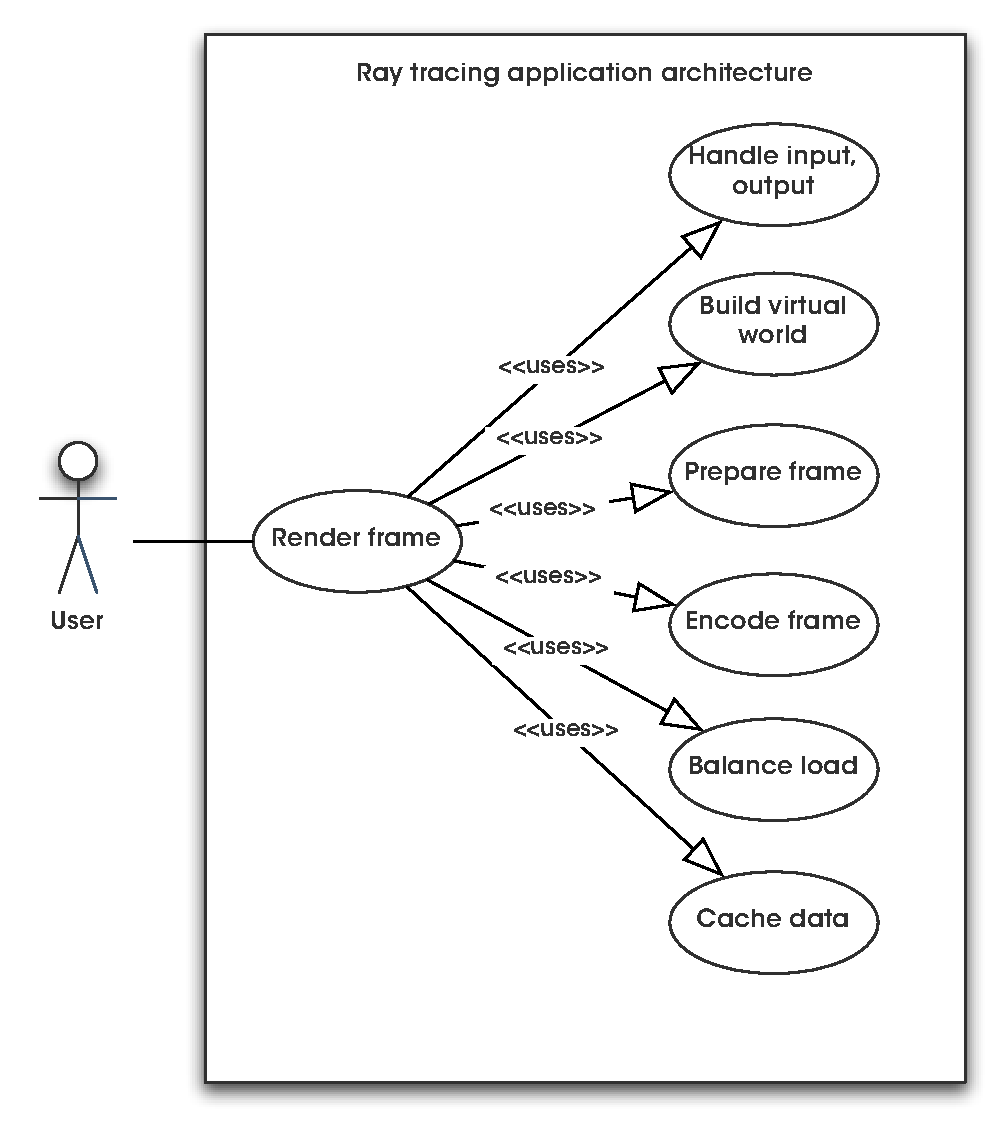
\includegraphics[width=0.6\textwidth]{diagramme/use-case}
\caption{Use case diagram}
\label{fig:usecasedigarm}
\end{figure}




\newpage
\section{Identifying an Appropriate Programming Model}
\label{sec:analysis_programming_model}
The next section will introduce various programming models for the Cell
Broadband Engine. Some of the models are specific only to the CBE others
are known from SMP systems. Identifying the appropriate programming model
is one of the first steps in developing for the CBE. It is an essential
task as the performance depends not only in the algorithms used as well as
on the data flow and in some way a programming model describes how data
is replicated repsectively distributed among the SPEs.

The determining factor of choosing the right programming model is how and when
 data can or must be made available to the algorithms executed in the SPEs.
Taking for example a rendering pipeline in which each SPE contributes
a specific part to the result, it would be inappropriate to choose here
the shared memory model as the result has to be written to main memory
and the successive SPE has to read it back at every stage of the pipeline. For
short pipelines it would be adequate but with the increasing number of stages
accesses to main memory would slow down the computation.

Another thing to consider here are the capabilities of the hardware and how
these capabilities can be exploited in conjunction with the programming model
and the data flow. Taking back in mind the example of the pipeline with the
shared memory model it was necessary to involve the main memory to store
the temporal results. This involvement can be nearly completely discarded as
the Cell BE is capable of writing and reading data from local store hence
the algorithm can directly store the result in the very next SPE for further
use. The advantage here is that results reside as long as possible in the SPEs
and are not circulated between local store and man memory. The pipeline model
would be here more adequate and more efficient.

This consideration were taken from the data point of view but if the code
is minimal compared to the moved data it may be more efficient to move
code to data instead of moving data to code.

Another big issue are the hardware constraints which exist on the hardware.
The biggest constraint is surely the local store. A significantly part of the
design process consists of considerations how data or code is moved to and from
the local store as there are \textit{only} 256Kbytes available for program, stack,
local data structures and DMA buffers.

The next subsections will explain briefly each programming model and how they
apply to the Cell BE. At the very end the choice of a programming model
for the application architecture will be made and the reasons described for
the decision made.


\subsubsection*{Function offload model}
The SPEs are used as accelerators for certain performance critical parts of the
algorithm. The main application is run on the PPE. Complex or performance
critical parts of the algorithm are offloaded to the SPEs. The main logic of
the application running on the PPE stays unchanged. The parts which are
offloaded are compiled with a special compiler and embedded into the PPE
executable. The call of one of these functions is transparent and looks or
behaves like a normal library function call. The developer statically identifies
which parts or procedures should be executed on the PPE and which on the SPE.

\subsubsection*{Device extension model}
In the device extension model the SPEs provide the function previously
provided by a device or act as an intelligent front end to an external device.
This model uses the signalling and event facilities of the Cell between the PPE
and SPEs as command/response First In First Out (FIFO) queue.

The Direct Memory Access (DMA) engine can map device memory into the address space
of SPEs and hence allows the SPE to interact with any device. The DMA engine even
supports transfer size granularity down to a single byte. In the case of an
intelligent front end provided by a SPE the devices can use the event facility to
quickly and efficient inform SPEs of completionn of arbitrary commands. Even small
messages between the device and the SPE can be exchanged by utilizing the mailbox
facility \cite{Kahle05}.

There is a special case of the device extension model where only a small
portion of the local store is available for communicating with the SPE. The
remaining portion cannot be accessed by any other device. This is used to
establish a trusted vault with which such functions as digital rights management
can be supported \cite{Kahle05}.

\subsubsection*{Computational acceleration model}
The computational acceleration model is SPE centric and provides a granular
and integrated use of SPEs. The most computationally intensive sections of the
code are performed on SPEs. The PPE acts primarily as a monitoring or control
system to the SPEs. The work is executed in parallel and has to be
partitioned. The partitioning can be done manually by the programmer or
automatically by compilers.

The partitioning plays a major role in performance issues. The developer has
to take into consideration that only an efficient scheduling of DMA operations
for code and data movement to and from the SPEs will result in maximum
performance. By using this model the developer can take advantage of the shared
memory programming model \cite{Kahle05}.

\subsubsection*{Streaming models}

In this model the PPE can act as a stream controller and the SPEs act as the
stream data processors. The SPEs can be setup as a serial or parallel
pipeline. Each SPE contributes a specific portion of computation to the data
that streams through the SPEs. This constellation can be very efficient if
each SPE has to do an equivalent amount of work since the data remains inside
the processor as long as possible.

In some cases it may be more efficient to move code to data instead of the
more conventional movement of data to code \cite{Kahle05}.

\subsubsection*{Shared Memory Multiprocessor Model}
In the shared memory multiprocessor model the SPE and PPE units can
interoperate fully in a cache-coherent shared memory programming model. All DMA
operations are cache coherent with respect to the SPEs. The conventional
shared memory load is replaced by the combination of a DMA fetch from main
memory to local store and  additional a load from local store into the register
file. In analogy to the load the store is replaced by a store from the register
file into local store and a DMA  operation from local store into main memory.
Equivalents to the power architecture atomic update primitives are also
provided by the SPE units by utilizing the DMA lock line commands.


\subsubsection*{Asymmetric thread runtime model}
The asymmetric thread runtime model is analogue to the conventional symmetric
multiprocessing (SMP) model.
Threads can be scheduled to run on either the PPE or the SPEs and the
interaction between them is similar to SMP systems. The asymmetric thread
runtime model is an extension to the lightweight models of modern operating
systems. The model includes processing units with different instruction sets
such as the PPE and SPE.
To optimize performance various scheduling policies can be applied to the
threads of the PPE and SPE.

This runtime model is very flexible and can support all of the previously
mentioned programming models \cite{Kahle05}.

\subsection{Programming Model for the Application Architecture}
\label{sec:programming_model}
The choice of the \textit{right} programming model is as mentioned before an
essential task in the development process. Not only the data flow has to be
considered also the architectural features of the Cell BE. To fully exploit this
architectural features it is recommended  to follow designated software strategies
and techniques that are specific to Cell.  Therefore as an addition to the
considerations about the data flow these techniques are also taken into account.\\\\


The strategy here used is to firstly name the factors that influence the decision
for a programming model in the context of ray tracing. Secondly each programming
model with its advantages and disadvantages are evaluated for its capability.

\subsubsection*{I. Data Flow}
\label{sec:data_flow}

A highly efficient data flow can increase performance drastically. The data flow
includes all movement from and to the local store. It depends if the data is fetched
from main memory or from the local store from another SPE as the bandwidth is higher
from local store to local store as from local store to main memory. Various algorithms
produce results which have to be  distributed among other processors so it is
important to consider the synchronisation of data.

\subsubsection*{II. Architectural Features}
\label{sec:arch_feat}

\subsubsection*{Computational Power}
Computations that are not well suited for the SPEs, like branchy scalar code,
should be best offloaded. The SPEs are the \textit{workhorses} of the CBE and
therefore they should be used as data plane processors performing all the
heavy computational parts \cite{Brokenshire06}. In addition to the computational
power of the
SPEs is the fact that there are eight times more SPEs as PPEs. The PPE should be
used as a control unit that orchestrates the SPEs and assists them in
synchronization, work assignment and representation of the results whether in
graphical, textual or any other way.


\subsubsection*{Communication and Event Facilitiy}
The Cell BE posseses a set of channels that are used as the primary interface
between the SPUs and the MFC. the SPU Instruction Set Architecture provides a
set of channel instructions for communication with external devices through a
channel interface. This channel interface facilitates each SPE to communicate
with other SPEs and the PPE. Besides two signalling channels there exists a
mailbox facility which is used to exchange small messages.

The event facility is capable of monitoring many events which occur during
processing. This includes of course the signalling and mailbox channels.
Each signal or mailbox message respectively event can be processed and made available
for SPE disposal. The flexibility of the event facility can be further exploited when
used as a synchronization utility,  message passing interface or as intelligent
frontend to an external device.

\subsubsection*{Programmer Managed Data Transfers}
The developer has full power of data transfers. The developer decide when and where data
is stored.  With memory mapped input output (MMIO) it is even possible to access local
stores, signalling channels and the mailboxes of other SPEs. This forces the developer
to be aware of all data accesses and encourages thought of regarding application data
access patterns but this also allows a programming with great flexibility.

\subsubsection*{III. Hardware  Constraints}
\label{sec:hardconst}

The SPE local store is a limited resource. 256Kbyte is available for program,
stack, local data structured and DMA buffers \cite{Brokenshire06}. It also used
for local caching and temporary data. The problem of to large program code can be
avoided with code overlays. The CBE programming manual speaks of plugins
\cite{IBMhb06}.

For memory bound applications it is better to keep data transfers, communications
and synchronization on chip and not consume memory bandwith as the Element
Interconnect Bus (EIB) provides
significantly more bandwidth than system memory.

There are further things to consider but they do not affect the choice of an
programming model. They are bound to the algorithm, like the SIMD strategy used,
branches, instruction set and issue rules, pipelining, dual issue, double
buffering and prefetching. Further improvement can be achieved with the correct
design of data structures for efficient accces, huge tables and locking but these
things will be considered for the ray tracing core in section \ref{sec:design_rt}
here the consideration take place on a higher level.


The above consideration are now modelled as weighted factors which will affect the
choice of an programming model. The range of the weight will be between 1 and 10
depending on the importance to the ray tracing algorithm and the perfromance issues.
The table \ref{tab:factors} shows the weighted factors and the assignment to each
programming model. It must be clearly said that this factors and its assignment
should not be seen as an general representation, here it is always in the context
of ray tracing. The device extension model and the asymetric thread runtime models are
for further  consideration exluded as the device extension model acts as a device
and the asymetric thread runtime model is just a generalization of the others.
Furthermore the computational acceleration model cane take great advantage of the
 shared memory programming model hence there are really three competing programming
models. The first the function offloading model, the second the shared memory
model and last the streaming respectively pipeline model.

\begin{table}[h]
\centering
\begin{tabular}{|c|c|c|c|}
\hline
\textbf{\textsf{{Weighted Factors}}} &
\textbf{\textsf{\textbf{Function Offload}}} &
\textbf{\textsf{\textbf{Streaming Model}}} &
\textbf{\textsf{\textbf{Shared Memory Model}}} \\
\hline
Offloading      & 5  & 9   & 10 \\ \hline
Parallelism     & 8  & 10  & 10  \\ \hline
Data Flow       & 3  & 6   & 8  \\ \hline
Communication   & 8  & 7   & 8  \\ \hline
Caching         & 6  & 8   & 9  \\ \hline
Load Balancing  & 6  & 6   & 7  \\ \hline
Sum             & 42 & 46  & 50  \\ \hline
\end{tabular}
\caption{The decision-making table with the weighted factors}
\label{tab:factors}
\end{table}

The first factor to consider was \textit{offloading}. The whole ray tracing process
is computational itensive hence it was important to offload as much, actually all work
onto the SPEs  as possible. The function offload model (FOM) uses the SPEs as
accelerator for certain performance critical parts of the algorithm and not the
whole one. The streaming as well as the computation acceleration modell are capable
of offloading the whole algorithm to the SPEs and the SPEs are performing all the
heavy computationl lifting. Besides the fact of offloading the streaming model
has one penalty, the PPE must or can act as a stream controller either balancing
the load and assigning new workload to the SPEs. The shared memory model facilitates
the SPEs to full featured autonomous ray tracers which can operate independent hence
the offloading is fully exploited.

The second factor \textit{parallelism} describes how the programming model is capable
 of executing specific parts in parallel. Both the streaming modell and the shared
memory model exploit parallelism at higher degree as the function offload model in
 the context of ray tracing. For example
doing 8 intersections tests at the same time is a difficult task as the traversing
through the grid, the intersection test and  the shading is modelled for one ray.
In the streaming model these task are accomplished in a sequential manner horizontally
through the SPEs  and in  the shared memory model in each of the SPEs at the same time.
One important thing which should be mentioned in the sake of parallelism is the fact
that in the streaming model the SPEs always depends on the data from the very last
SPE and has to wait for completion.


A major obstacle in distributed computing is the \textit{data flow}. The main object
 is to
keep data as long as possible on the CPU, workstation, blade or whatever the node
 is. Taking back in mind the pseudo code of ray tracing it is obvious that
ray tracing is a chain of stages that are interconnected and depend on each other.
As mentioned before each stage needs the results of the previous stage to finish
the actual stage. The streaming  model is a interconnected chain of SPEs just like
 the ray tracing algorithm. At the first sight it may seem as the most advantagoues
but the problem which yields out of
the streaming model on the Cell BE is that beside the access to local store there is
always a access to main memory involved. Furthermore the data distributed
distinguishes from SPE to SPE the PPE has to take care of it and make the various
data available for SPE disposal.
For the function offload model the specific data has to be made
available for each offloaded function and the results retrieved. There would be
a constant pushing an popping of data for each stage of ray tracing.
The autonomus approach of ray tracing on a SPE has the advantage that intermediate results
have not to be distributed to other SPEs. This model exploits the \textit{stay on chop}
constraint at the highest degree. The minimal input is negligable as it is
retrieved once and used for consecutive frames. The output at last are the completely
rendered tiles.


In ray tracing is doesn't matter how the work is partitioned, tiles, rays, object groups
..., the workload is always unpredictable. If it is possible to minimize either the load
 balancing or the work assignment or decouple the PPE completely from such tasks would
be helpful. The responsibility of work assigment and load balancing in the function
offload as well as in the streaming model takes the PPE. In the streaming model
the load balancing could be decoupled from the PPE but additionally to the balancing
the load balancing algorithm has take care of heterogeneous results. For example the first
step is the generation of the primary rays. The result is a ray which is distributed
to the very next SPE. The second step performs intersection tests and distributes the
point where  the object was hit and the incident ray and so on.
In the shared memory model the load balancer has to deal with only one \textit{data type},
the tiles. The granularity of tiles are pixels which are the smallest tokens to distribute.
It is obvious that with tiles we have a unique data type and large choice of magnitudes
that can be distributed among the SPEs.

Another thing to consider is how much communication overhead is produced during the
 processing. An unfavorably strategy could slow down all SPE and prevent them from
efficient computation. The communication facility of the Cell BE is firstly used
to synchronize the SPEs. An load balancing strategy is not efficient when a highly
amount of processing power is consumed in communicating and migrating work from on
SPE to another. Therefore the communication overhead should be minimized to the lowest
level. The problem which arises is that all models in the context or ray tracing need
a load balancer. In the function offload and streaming model the communication is
centralized to the PPE. The PPE acts like an proxy to the other SPE. In the shared memory
model the PPE can be completely decoupled and so communication overhead is minimized.

The last thing is the aptitude for caching. All three models would gain performance
improvement through a cache as every needed data is hold in the local store for future use.
The big advantage of the shared memory modell and the conjunction with a cache is
that not only spatial as well as temporal coherence can be exploited. For a detailed
description see section \ref{sec:demand_analysis}.

\subsection{Conclusion}
The application architecture will use the shared memory model as it has advantages
over the other programming model. The data stays on chip as long as possible, with
the cache the coherence  is exploited, thrashing of pages are reduces as the cache
stores a big amount of objects, material and lights. Furthermore the communication
overhead is reduced as the PPE can be completely decoupled from the load balancing
and work assignment.

\newpage
\section{Ray Tracing Accelerating Techniques}
\label{sec:accel}
Ray tracing is one of the mostpopular methods in computer graphics and probably
everybody experienced in 3D graphics knows and use it. The simplicity of Ray
Tracing has attracted many people to implement it with the highest possible
efficiency. Despite its impressive repertoire, Ray Tracing is often
dismissed
as being too computationally exorbitant to be useful in the professional field
of use. On many conferences software and hardware improvements have been
presented over the last 20 years. This led to different approaches involving
many different algorithms to speed up ray tracing. The figure
\ref{fig:rayacceltech} shows a general overview of algorithmic acceleration
techniques.

\begin{figure}[H]
\centering
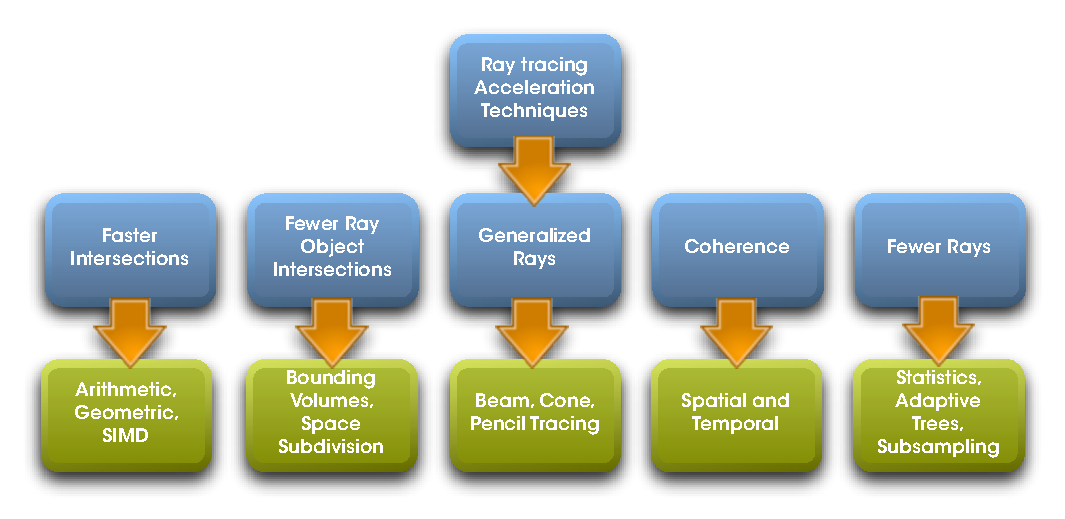
\includegraphics[width=\textwidth]{diagramme/raytracing_acceleration_techniques}
\caption{A broad overview of ray tracing acceleration techniques \cite{Glassner89}}
\label{fig:rayacceltech}
\end{figure}

The next section will introduce the most popular techniques for speeding up the
whole ray tracing process. To describe all acceleration techniques would go far
beyond this work. For a deeper overview see \cite{Wald04} \cite{Glassner89}. The
techniques can be divided up in pure computational improvements and algorithmic
improvements. The pure computational improvements can be added to existing source
code and used without any special additional data structures. The algorithmic
improvement need heavy changes in existing source code and maybe need additional
data structures. The next section will introduce techniques which are well
documented and tested in various papers and ray tracers.

\subsection{Faster Intersections}
Intersectors are extremely quick routines for computing intersection between a
ray and a certain object. There are two main types of intersection tests. On the
one hand there are the arithmetic tests, which just equate the function of the
ray with an object. The main disadvantage of arithmetic tests is that there is
no effective hit/miss tests which allows to reject an object sooner than the
real intersection point will be analytically computed. On the other hand there
are the geometric tests which have a effective and fast rejecting policy. This
is especially important for complex objects like triangle patches, which can
consist of many triangles. On special hardware like modern CPU's the developer
can take great advantages by using the vector units which can operate on
multiple data with a single instruction also referred as SIMD. For example the
grouping of 4 Rays to a packet can increase the performance by a factor of 2-3.

\subsection{Fewer intersections}
The main purpose of the following algorithms is to decrease the number of
intersections. It is known that 95\% of computing time are intersection tests
and there is a big performance speed up if a significant number of intersections
can be avoided.
\subsubsection{Bounding Volumes}
Bounding volumes can have a notable speed up in refusing complex objects which
are missed by the ray. The cost of additional memory needed is affordable in
comparison with the savings in computational time. Imagine a triangle patch of
about 3000 triangles. Now if the bounding volume is intersected, commonly a box
or sphere, 2999 intersection tests can be discarded. Most bounding volumes are
simple geometric primitives like spheres and boxes with fast intersectors which
can reject rays very fast, as mentioned in the previous section. Even complex
bounding objects can be used for intersection tests. The biggest problem is
caused by narrow long objects, their bounding volume contain most of the scene
and add more overhead than without it. Bounding volumes can be arranged in a
hierarchical data structure to achieve yet more performance.
\subsubsection{3D Spatial subdivision}
The main problem in ray tracing is finding the nearest intersection
point for each ray. Rays can have arbitrary directions and there is no chance to
sort all objects to a list which will be somehow useful during tracing a ray.
The only possible solution is to organize the objects into groups depending on
there relation, either by space occupied or neighbouring relation. Rays are then
tested with a small subset of the objects.

There are two general strategies for space subdivisioning. The first strategy
are hierarchical bounding volumes. They achieve higher efficiency by grouping
objects into bigger groups. Before intersecting the complex object, the bounding
volume respectively outer bounding volume which encloses the whole group of
primitives and which is some kind of convex hull to the objects within the
volume, is intersected. Actually no intersection point is calculated, it is just
tested if the ray hits the bounding volume, not where. If there is no
intersection there is no need to intersect the ray with the complex object.

\subsubsection{Bounding Volume Hierarchy}
Around a complex scene made up of many objects a bounding volume is placed
around the entire scene. Each object also contains a bounding volume. The
bounding volume hierarchy can be represented in a tree structure. Each node
contains a bounding volume which enclose its children nodes. The leaves contain
precise information about the object and there is no redundancy of such data.
The amount of intersections are reduced but now time is spent intersecting
bounding volumes with all objects contained in the scene. The creation of the
bounding volume hierarchy is the main impact of speed up.

\subsubsection{Uniform Space Partitioning}
\label{sec:uniform_space}
The second strategy is to partition space itself into regions or voxels. The
word voxel is an abbreviation for volume element and pixel. Each voxel contains
a list of objects which lie in the voxel. Long objects span more than one voxel
thus they are in more than one list. The starting point is the voxel in which
the ray originates. If the ray hits any object in the starting voxel the
intersections are sorted and the closest is retrieved. If the closest
intersection is in the current voxel there is no need to intersect any other
objects because the closest intersection if fount and the objects behind
are occluded by the hit object. If no intersection is found in the current voxel
the ray is traversed to the neighbouring voxel. This process is continued until
an intersection is found or the ray completely traverses the space partition.

The traversed voxels describe a rough way along the direction of the ray. Only
objects that occur along the ray are intersected. Object far from the ray are
not taken into consideration and are trivially discarded. The number of
intersections are vastly reduced.

Two popular space partition schemes were developed. The first are octrees by
Glassner \cite{octrees}, where voxels are of different size and contain almost
one object. This approach saves space, since there are as many voxels as
objects. The biggest drawback is the difficult traversal through the voxel.

The second is constant size voxel partitioning by Fujimoto \cite{IBMhb06}.
Each voxel is of same size and contains a object list. This strategy allows
simple traversal at the expense of more voxel. Furthermore the algorithm can be
expanded to coherent grid traversal by Wald \cite{Wald06Grid} which accelerates
the grid traversal by more than a factor of 10, and achieve ray tracing
performance competitive with the fastest known packet-based kd-tree ray tracer.

\subsubsection{kd-Trees}
Kd-trees are a special case of BSP\footnote{Binary Space Partitioning}-trees.
The space is recursively subdivided into convex sets by hyperplanes. These
subdividing is done with splitting planes that are perpendicular to one of the
coordinate system axes contrary to octrees \cite{octrees} where the splitting
planes are fixed and to BSP-trees in which arbitrary splitting planes can be
used. The splitting planes of a kd-tree are determined by a heuristic which
is essential to kd-tree building \cite{Havran2000:PhD}. Chosing a good
heuristic will improve the bulding of the kd-tree
significantly \cite{wald:06:NlogN}.

In ray tracing kd-trees are used as follows. The main disadvantage of uniform
spatial subdivision is that geometric primitives can span over multiple voxels
and reside in several lists. Furthermore it happens often that there are is a
big amount of voxels that do not contain any primitives and are thus unnecessary.

Kd-trees try to overcome this situation by generating voxels that
contain only one or as less geometric primitives as possible. If the
space does not contain any object the space is not further subdivided.

Kd-trees and Octrees fall into the categorie of adaptive trees that is a major
field in accelerating ray tracing. For further references see
\cite{Havran2000:PhD}, \cite{wald:06:NlogN} and \cite{Glassner89}.

\subsubsection{Light Buffers}
Light buffers are used to decrease the time needed for the evaluation of shadow
rays \cite{light-buffer}. The idea is to surround each light source by a cube
covered by a rectangular grid. The complete list of objects
that are projected in a preprocessing step to each grid cell is sorted and
stored. If there is an object covering a complete area of cell, all objects
more distant from light are removed. If there is only one object it is removed
because it occludes no other object. When a shadow ray is processed, the
appropriate grid cell is selected and a position in the list of candidate objects
 is determined by a distance from a light source. Only the possible occluders
between a point and light source are tested for intersection. Light buffer
exploit coherence of shadow rays. Although they are sent form various places in
a scene all rays are directed at the same targets, the light sources.

\subsubsection{Shadow Buffers}
Shadow buffers are used to decrease time needed for finding the closest
occluder firstly introduced by \cite{light-buffer} and extended by
\cite{shadow-buffer}. After processing the  shadow ray the occluder is stored in
the shadow buffer.
If one point is in shadow, then the next point will almost certainly be,
too. So the next shadow ray is first intersected with the objects in the shadow
buffer. If there is an intersection the tracing can be stopped. Otherwise the
remaining objects have to be checked. Shadow buffer also exploits coherence
similarly to light buffers. Neighbouring points are gone to be occluded by the
same objects and lid by the same light sources. A cheat would be to only do a
shadow check every second pixel, and if one is in shadow then assume the next
point is in shadow, too, and skip the shadow check.

\subsection{Fewer Rays}
This section will introduce some techniques to reduce the number of rays
shot into the virtual world. Fewer rays are one of the major strategies
to improve performance of a ray tracer.

\subsubsection{Adaptive Tree Depth Control}
Adaptive tree depth control allows easily to reduce the number of rays
intersecting the objects in the virtual world. This method not only includes
primary rays but also rays which are the result of recursive generation of
refraction, reflection and shadow ray calculations.

Instead of terminating the ray tree\footnote[1]{The ray tree represents the
primary and the recursive generated rays. Every hit, a node, produces a
refraction, reflection and shadow ray (based on the surface properties) which
are the leafs of the tree. Every ray can produce further rays. }
 at constant tree depth a threshold intensity is
used to stop further generation of rays. The difference between these methods
is that the constant tree depth does not take into account that secondary rays
can have a big color contribution to the actual pixel and are discarded because
of the limited tree depth. Furthermore an opaque or lambert surface has no
reflection or refraction intensity contribution and it is unneccessary to
compute secondary rays to the specific tree depth was.

This estimation first introduced by Hall \cite{HallTreeDepth83}. He presented
a termination criterion which takes into account the contribution to the actual
color of the pixel by continuing the recursion. It is possible to discard the
generation of secondary rays deep in the tree which have no significant
intensity contribution, without altering the result.

Adaptive tree depth control saves a lot of computation especially with opaque,
lambert and nonreflecting surfaces.

\subsubsection{Adaptive Anti Aliasing}
If there are larger areas with the same or similar intensity the calculation
of neighbouring pixels can be avoided with adaptive anti aliasing. In place of
sending one ray per pixel, for every n-th pixel a ray is generated and the
intensity computed. Rays for pixels in between are only generated if the
threshold differ in a certain intensity otherwise a linear combination is
computed and applied. The advantage of this approach is that rays for pixels in
between have not to be evaluated.

Adaptive anti aliasing can save a big number of primary rays for areas with
similar intensity like the background, planes and big homogen objects. The main
disadvantage is that very small objects can slip thru the raster if the
intervall of pixels is to big.

\subsection{Adaptive Sub Sampling}
Adaptive sub sampling is a similar technique as adaptive anti aliasing. This
time the algorithm is not applied on anti aliased pixels but on normal pixels.

As stated in the section adaptive anti aliasing a big number of primary rays can
be saved. As the algorithms are the same the same advantages and disadvanteges
result of this approach.

\subsection{Statistics}
Statistics in ray tracing are used to reduce the expense of computing and drawing
samples. Only enough samples are drawn that produce an estimate of the desired
accuracy. There is always a degree of uncertainty in such estimates. The
precision of such estimates, which can be arbitrary, may however be more accurate
by computing a large number of samples. Such a method is stochastic sampling and
is described in \cite{Cook86}. With stochastic sampling effects like motion blur,
penumbrae, depth of field and dull reflection are provided. An extension to the
rendering equation made even caustics and diffuse interreflection of light
between objects possible \cite{Kajiya86}.
The stochastic sampling method calculates reliable estimates via Monte Carlo
integration.

Monte Carlo methods are used for simulating the behavior of various physical
and mathematical systems. They are nondeterministic and stochastic contrary to
other systems like methods of molecular dynamics. These behavior results of
using pseudo random numbers in calculations as opposed to deterministic
algorithms.

\subsection{Generalized Rays}
The simple form of the rays  allows the simple representation, efficient
intersection caculations and great generality, but the representation of a ray
as infinitesimally thin rays causes problems when applying calculations on
anti-aliasing and the exploiting of coherence. One way to overcome these
problems is the use of generalized rays. Generalized Rays consider an entire
family of rays bundled as beams, cones or pencils.

On the on hand some sacrifice is required to use each of these generalized rays.
The types of primitive objects may need to be restricted and the computation of
exact intersections may need to be abandoned \cite{Glassner89}. On the other
hand the use of generalized rays leads to advantages such as increased efficiency
by exploiting coherence, effective anti-aliasing and additional optical effects.


\subsection{Coherence}
Especially in ray tracing coherence is a property which can be found in many
places. The spatial coherence plays a major role in issues on performance
regarding ray tracing. ray tracing parts like rays, pixels, objects and lights
are either constant or only change partially. The values change in a predictable
manner so it is possible to utilize coherence. Before utilizing it is essential
to understand the algorithms used and to find similiarities and continuities.

Higher speed of computation can be achieved with the knowledge of data coherence
since many routines process the same or similiar data sets. Coherence
can be found in many places regarding ray tracing.\\\\
\textbf{The following list shows the different types of coherence found in
ray tracing}
\begin{description}
\item[\color{Bigblue}{$\triangleright$}] Ray coherence
\item[\color{Bigblue}{$\triangleright$}] Image/Pixel coherence
\item[\color{Bigblue}{$\triangleright$}] Object coherence
\item[\color{Bigblue}{$\triangleright$}] Frame coherence
\end{description}

The different types of coherence can be summarized into two groups. First of all
there is spatial coherence. To the group of spatial coherence belongs ray,
image/pixel and object coherence. The second group is temporal coherence where
frame coherence belongs to.

\subsubsection{Spatial Coherence}
\label{sec:coherence}
Spatial Coherence describes all places in the context of ray tracing that
have no temporal character. As beformentioned there are several types of
coherence which can be exploited to design algorithms which perform better than
exhaustive ray tracing.

First of all there is ray coherence which expresses the fact that similar rays
with the same origin and similar direction will trace similar paths through the
grid either uniform or non-uniform and hitting  the same objects which  lie
nearly in the same place.

Object coherence expresses the fact that objects consists of pieces which are
connected, smooth, bounded and that distinct objects tend to be largely
disjoint in space. There are not typically intermingled clouds of randomly
scattered fragments \cite{Glassner89}.

Image/Pixel coherence expresses the fact that neighbouring pixels are constant or
only change partially and techniques such as subsampling can be applied. The
attributes of objects in the 3D space are carried into the 2D image. All
attribute like smoothness, connecteness remain unchanged.

As an example, adaptive anti aliasing takes into account that neighbouring
pixels either are constant or only change partially. The property of pixel
coherence can be expanded not only to the spatial point of view also to the
temporal point of view\footnote{For realtime ray tracer it is important not
only to consider spatial but also temporal coherence.}. The next section will
give a brief description of spatial and temporal coherence found in ray tracing.


Coherence is often exploited even without knowing it. An example is the spatial
subdivision techniques. The reason why spatial subdivision works is
the property that small voxels tend to intersect relatively few objects in the
environment. That means that the whole scene can be partitioned into smaller
amounts of objects, the objects are locally seperable which is an attribute of
object coherence\cite{Glassner89}.

On the opposite side, if it is assumed that objects represent a intermingled
cloud of randomly scattered fragments and don't have the attribute to be
seperatable the spacial subdivision would gain no benefit compared to exhaustive
ray tracing.\\
For a deeper introducton see \cite{KaplanM87} and \cite{ChapmanCalvertDill90}.

\subsubsection{Temporal Coherence}

Temporal Coherence is an important fact considering interactive rendering.
Ray tracing , global illumination as photon mapping as well as radiosity
can take great benefit of frame coherence. It describes the
fact that the difference between frames is exiguous if the time interval is
small. Frame coherence is based on object coherence but with an temporal
character. Objects like light sources are not changing dramatically
between two successive frames and the major part of the picture can be reused.


\subsection{Considerations for the Ray Tracer}
For the  new ray tracer almost all acceleration techniques will be used. For faster
intersection test the arithmetic tests are converted to geometric and are SIMDized.
To achieve fewer intersection test the uniform space partitioning scheme will be used.
Since it is simple to implement and has a incremental character. The latter point
is very important since the CBE has no branch prediction and limited local store
which forbids recursive calls to functions. Kd-trees are not considered in the frame
of this work since finding a good heuristic and implementing a kd-tree would take too
much time \cite{Havran2000:PhD}.

The coherence in ray tracing is exploited with the
use of the cache and the programming model for further information see section
\ref{sec:demand_analysis} and \ref{sec:programming_model}.


Fewer rays are achieved with the use of adaptive tree depth control. Adaptive anti
aliasing or adaptive sub sampling are note used because they can yield to falsified
pixel values.

Stochastic sampling methods are note considered in the frame of this work as
they do not contribute a significant performance increase they could even
decrease the performance when using the extended rendering equation by
\cite{Kajiya86}.



\newpage
\section{Ray Tracing Engine}

This section will analyize the various parts of the ray tracing engines and provide
solutions which arise due to hardware constraints on the Cell Broadband Engine.
Some parts will be offloaded completely to the SPEs, some will only reside on
the PPE.
\subsection{Input/Output Handling}
The result of the rendering process will be shown in a graphical window. The graphical
output is the main interaction point betwwen the user and the system. The user should
be able to move in the virtual world in real time. To accomplish this task an graphical
abstraction layer will be used which takes care of the video output, keyboard
interaction and update of the frames.

\subsubsection*{OpenGL}
OpenGL (Open Graphics Library) is a standard specification defining a cross-language
 cross-platform API for writing applications that produce 3D computer graphics (and 2D
computer graphics as well). The interface consists of over 250 different function calls
 which can be used to draw complex three-dimensional scenes from simple primitives.
OpenGL was developed by Silicon Graphics and is popular in the video games industry
where it competes with Direct3D on Microsoft Windows platforms (see Direct3D vs.
OpenGL). OpenGL is widely used in CAD, virtual reality, scientific visualization,
information visualization, flight simulation and video game development \cite{opengl06}.

The OpenGL library alone is not capable of handling system level I/O as for example
keyboard and mouse interaction. Therefore an extension must be used to facilitate
OpenGL for I/O. A widespread library in conjunction with OpenGL is the OpenGL
Utility Toolkit (GLUT).

The OpenGL Utility Toolkit (GLUT) is a library of utilities for OpenGL programs,
 which primarily perform system level I/O with the host operating system. Functions
performed include window definition, window control, and monitoring of keyboard and
mouse input.  The two aims of GLUT are to allow the creation of rather portable code
 between operating systems (GLUT is cross-platform) and to make learning OpenGL easier.
Getting started with OpenGL programming while using GLUT often takes only a few lines
of code and requires no knowledge of operating system \cite{glut06}.

\subsubsection*{Simple DirectMedia Layer}
The Simple DirectMedia Layer is a programming application programming interface
(API) for developing games, demos and multimedia applications. SDL provides an interface
which enables the developer for easy use of the graphics card, sound, joystick or
keyboard. There is no need to actually know how to put an image into the
framebuffer or how to display it the Simple DirectMedia Layer takes care of it.

If SDL is mentioned it is often compared to Microsoft's DirectX. From the technical
point of view there is not much in common but to understand the SDL philosophy it
can be seen as a multimedia interface such like DirectX.

The main advantage of SDL is the portability and it is Open Source.  SDL is available
for a wide range of plattforms even for such exotic as the Sharp Zaurus, Sega Dreamcast
or the Playstation II. The interface is always the same. Applications which are developed
for example on Linux can be compiled under windows with no code modifications.

The SDL can handles a wide range of multimedia as for example video, audio, input output,
truetype fonts, images and so on. It can even be used as a frontend to various
graphics libraries like OpenGL, Mesa or Allegra. SDL reconciles all the powerfull
libraries for easy of use.


\subsubsection{Graphical Output}
\label{sec:analysis_graph_out}
The Simple DirectMedia Layer provides a abstraction mechanism for framebuffers and
supplies procedures for effective access. When no hardware framebuffer is available
the Simple DirectMedia Layer emulates the hardware by a software framebuffer, in
SDL referenced as surface. This surface is actually more than just a framebuffer it
is  a general purpose canvas which holds several pixels, images or fonts. Furthermore
any number of surfaces can be allocated and used. This provides a flexible
setup as each surface holds miscellaneous data and this can be blitted into the
destination surface, the framebuffer.

This flexibility is important as the actual hardware setup on the Cell-Blades do not
provide a hardware framebuffer, they lack of an graphics card. Furthermore the SPEs
are not capable of using the procedures provided by the SDL or accessing the surfaces
directly. The SDL is highly dependent on an operating system (in this case Linux)
 and as a
consequence only the PPE can use the Simple DirectMedia Layer.


The solution to this problem is that the PPE allocates a extra surface which will
be used by the SPEs. The surface is as block of memory which holds pixels in a
defined format and can be easily written by the SPEs facilitating the MFC.
The resulting surface can be blitted by the PPE into the framebuffer and shown in
a window.

It is important that the pixels are written in a specific format. Therefore procedures
which are responsible for mapping the RGB values into the pixel format will be ported
to the SPEs.  From the SPEs point of view it will look like a call to the library but
it will be executed on the SPEs. Doing it this way preserves a consistent interface
and behaviour. For a general purpose use of the SDL further parts could be ported
but as the ray tracer only renders pxiels it is sufficient to port the pixel handling
procedures and leave the most part to the PPE.


\subsubsection{Event Handling}

An event in an application is used to control the program flow. Each event is coupled
with a so called event handler that is executed everytime when the specific event occurs.
A related concept are interrupts. Events are often used for graphical userinterfaces whereby
the events are often actions from the user like the press of a keyboard button or a klick
by the mouse. How each event is coupled to the handler and how the events are processed is
differentially and depends on the library used.

As beformentioned the Simple DirectMedia Layer also provides procedures for input
and output handling. The SDL has a sophisticated event handling mechanism that allows
an easy setup for processing mouse and keyboard events.

An event handling mechanism is necessary as the user should be able to navigate threw
the scene and move the camera. As beformentioned the SPEs are not able to directly
use the SDL library therefore the event handling and event sending must be split
into the PPE part and the SPE part. The PPE part will use the SDL event framework
whereby an event framework for the SPE has to be implemented.

\subsubsection*{PPE Event Handling}
The PPE event handling will provide handler for various keyboard shortcuts. These
shortcuts will trigger specific functions of the ray tracer. One key will be
used for triggering the informational output. On keypress it will turn on
or turn off the information displayed in the window. The camera or the position
of the viewer can be changed radial or planar. If there is a distinction in
 movement the user should be able to choose between these two modi. For navigation
 the arrow keys can be used. As the output is only a graphical window a key shortcut
 will be used to terminate the actual session. The event handling mechanism is similar
to graphical user interfaces and will be not further explained. For a deeper
introduction of the \textit{SDL Event} facility see \cite{SDL06}.


\subsubsection*{SPE Event Handling}
The SPE event handling framework will be highly based on consisting event
handling frameworks and concepts. Which means that for each event an event
handler is used and a central unit processes the events and delegates it
to the specific handler. One simplification will be done. In a modern
graphical user interface each event source can be coupled with several
arbitrary event handler. In the ray tracer a fixed assignment of event
source and event handler will be used. There is no need for higher abstraction
respectively generalization as the keyboard event should always call
the keyboard handler and events always be send to the ray tracer.

The main problem which arises here is the translation of events on the PPE
to events on the SPE. Helpfully the Cell BE has an sophisticated event
facility which can monitor the occurence of signals, mailbox  messages,
MFC tag-group updates and others. This event facility will be exploited
and partly used as a graphical user interface event handling facility.

Partly because the event facility can be further on used for synchronisation
,  interprocess communication or pipes for message exchange.

\subsection{Building the Virtual World}
There are many ray tracer available in the internet either commercial or free.
They have one in common. As many ray tracer exist as many description
languages for virtual worlds exist. It is a wide range of proprietary formats
which are incompatible with each other.

Therefore a description langauge will be used which already exists and has
an easy syntax. The POV-Ray ray tracer is the most known free ray tracer
with a distinct description langauge. The descpription langauge is used
to describe a virtual world that should be rendered with the ray tracer. The
main advantage of a description language is that it is not needed to modify
code for a new scene. The user simply modifies the scene file and the ray
tracer takes care of it.

For the ray tracer a compiler will be developed which understands the
POV-Ray description language and from their it builds up the virtual world
for use by the ray tracer. The POV-Ray description language is preferable
as the POV-Ray reference supplies the developer with the context-free
grammar of the language which is crucial for compiler development.

\subsection{Preparing the Frame}
\label{sec:analysis_preparing_frame}
\label{sec:analysis_prepare_frame}

The raw ray tracing algorithm is computation expensive. The \textit{heart}
of ray tracing is the intersection of objects with a ray is expensive and
can easily take up to 95 \% of the rendering time. Each ray has to intersect
each object in the scene unless some sort of intersectin culling is performed.

There are two general strategies for intersection culling, hierarchical bounding
volumes and space partitioning. For more information on intersection
culling see section \ref{sec:accel} for an introduction and section \ref{sec:render}
on the fast voxel traversal algorithm for the ray tracer.

The fast voxel traversal algorithm needs a preparation step before it can be
used. As stated in \ref{sec:render} the space itself is partitioned into regions
or voxels. Each voxel has a list of objects that are in the voxel. If an object
spans several voxels it is in more than one list. To sum up the preparation step
for the fast voxel traversal algorithm is the space partitioning and the assignment
of the objects to the corresponding voxels.

With the information supplied from the preparation step the ray tracer can now
traverse a ray through the grid and intersect the objects. It is clear that this
step has always be performed when objects change the position in the virtual world
as the lists in the voxels can or will change.

Several intersection test rely on precomputed values for example the barycentric
coordinate intersection tests and are also need to be prepared before the
actual ray tracing is preformed. This precomputation can also be done as a
preparation step.

\subsection{Rendering the Frame}
\label{sec:render}

In ray tracing there are three types of complexity to overcome. The first
is geometric complexity that describes the fact that for detailed scenes
many more primitives are used than can fit into memory. The second surface
complexity is a result of programmable shading and many texture maps. The
last is the illumination complexity which arises from realistic lightning
models and the interreflection of light.

Many ray tracing algorithms perform illumination computations assuming
that entire scenes fit in memory and simplify the lighting computation.
In distributed computing the entire scene has to be replicated along
the nodes. The replicated scene does not often fit into the memory
hence a strategy has to be developed for efficient computation. Therefore
the algorithms that compute accurate illumination with complex scenes
have to improve the coherence of scene data reference patterns.

Exploiting coherence to increase efficiency is a classic technique in
computer graphics. Increasing the coherence of a computation can reduce
the amount of memory used, the time it requires, or both \cite{Pharr97}.

The main idea for the ray tracing engine is based on caching. During
computation a subset of large geometric databases and material properties
are  cached in the local store of the SPEs for fast access by the ray
tracer. Data will be added to the cache on demand when needed for
computation.

To manage scene complexity the ray tracer will cache primitives
and the corresponding material properties. A limited amount of primitives
is stored in the local store and will be retrieved for the ray intersections
tests. When performing the illumination computation the corresponding
material properties are similarly saved and retrieved as the primitives.

The main feature of the cache is that it caches objects of arbitrary size
from 32-bit addresses to 128 byte cache-lines. Therefore the only limitation
of choosing supported primitives for ray tracing is that they do not
exceed the size of 128-byte. In the ray tracer for the Cell BE spheres
and triangles will be used as there are well documented intersection tests
and with triangle patches every shape can be modeled. There is no need
to optimize the caching by choosing only one primitive because the
retrieveal as well as the storing of primitives or any other object is
performed in the same time.

As stated in section \ref{sec:coherence} higher speed of computation can
be achieved with the knowledge of data coherence since many routines
process the same or similiar data sets.

The first measure to exploit coherence as well as to improve memory
coherence is to group rays into packets. All rays have the same origin
and consecutive rays will only change partially. The values change in
a predictable manner so it is possible to utilize coherence. The rays
in packet will probably intersect the same objects that has a positiv
impact on caching.
To exploit the coherence even more the ray packets are not rendered
randomly in a tile but in a confined area too.


The second measure for coherence is that ray packets are rendered
in a confined area. This means that the ray tracer renders a tile
of ray packets. This fact will influence the distribution and
redistribution of workload in the load balancing scheme used.

The third measure is the use of a generic cache. For more information
on the cache see section \ref{sec:cache}.

The use of a cache in the ray tracer for the Cell BE is crucial because
first of all the SPEs do not have direct access to main memory
and secondly the size of the local store is limited. The cache
has to supply the ray tracer at two specific procedures with data
from computation, in the traversal through the grid and shading
the actual pixel respectively applying the illumination to the
object.

In section \ref{sec:analysis_prepare_frame} it was mentioned that some form
of intersection culling should be performed to minimize the amount
of intersection tests. The fast voxel traversal algorithm for ray
tracing by \cite{Woo87} is a fast an simple voxel traversal algorithm
through a 3D space partition and will be used in the ray tracer. For
a deeper view see \cite{Woo87} or section \ref{sec:uniform_space}. As
a bonus of using the fast voxel traversal algorithm it can take great
advantage of the cache as the traversal incorporates the traversal
and the intersection tests.


After the traversal and intersection tests the actual pixel has to
be shaded. The shader with a specific illumination model takes
care of it.

\subsubsection*{Illumination Model}
\label{sec:shading_model}
What occurs when light strikes a surface is quite complex. It is a
continuous process in which light gets reflected, refracted or absorbed.
In true like light comes from inifinite angles and is reflected in infinite
directions.  The computational power which would be needed to accurately
 compute light like in true life would be immense. Therefore simplification
have to be done to accuratley to some degree compute the light.
The simplification shouldn't be to simple respectively to complicated. A
simple lightning model would deliver unsatisfied result on the other
side a too complicate model would last to long.

Hence a discrete model for lightning and illumination has to be supplied.
The intensity of a pixel is determined with a finite number of point
lights, reflections into space and illumination directions contrary to
true life.

A lighting model should entail lights, types of surface reflection
and should be discrete.


\subsubsection{The Hall Illumination Model}
\label{sec:hall_model}
\label{sec:analysis_hall_model}
The illumination equation of the Hall Illumination Model consist of
several light phenomena which summed up result in the intensity of
the rendered pixel. The light phenomena are differenced in the way
which object generated the light. Light from light sources is treated
with another equation as light which is radiated from other surfaces.
Furthermore the light is differentiated by the type of light. There is
ambient, diffuse reflection, specular reflection, specular reflection
from other surfaces, specular transmission from lights and  specular
transmision from other surfaces.

The following equation shows the components of the Hall Illumination
Model.


\begin{table}[h]
\centering
\begin{tabular}{l}
$I(\lambda) = k_{sr} \sum_j I_{lj}(\lambda) F_{sr} (\lambda, \phi_{r, j})
(cos \phi_{r,j})^n$\\
\hspace{1cm}$ + k_{st} \sum_j I_{lj}(\lambda)  F_{st} (\lambda, \phi_{r, j})
(cos \phi_{r,j})^{n'} $\\
\hspace{1cm}$ + k_{dr} \sum_j I_{lj}(\lambda)  F_{dr} (\lambda)(N \dot L_j)$\\
\hspace{1cm}$ + k_{sr}I_{sr}(\lambda)F_{sr}(\lambda, \phi_R)T_t^{\Delta sr}$\\
\hspace{1cm}$ + k_{st}I_{st}(\lambda)F_{st}(\lambda, \phi_T)T_t^{\Delta st}$\\
\hspace{1cm}$ + k_{dr}I_{a}(\lambda)F_{dr}(\lambda)$
\end{tabular}
\caption{A comparison of rays with hit and rays which are reprocessed}
\end{table}


\section{Cell Programming Rules}
The SPEs provide computational density advantage over conventional processors
through their programmability. Beside their programmability they provide
also greate flexibility contrary to application-specific integrated circuits
(ASIC) with its fixed function set.

The advanced instruction set and supported data types of the SPEs facilitates
the Cell BE to deal with a wide variety of applications. The developer is not
limited to a specific field of computation but can develop applications
for network processing, graphics, cryptography or high performance computing.

Near theoretical-maximum performance can be achieved for real applications on the
Cell BE processor unlike to conventional processors. The programmer must be
aware of the architectural characteristics of the processor to achieve
optimal performance \cite{Brokenshire06}.\\\\
The characteristics of the processor are:
\begin{description}
\item[\color{Bigblue}{$\triangleright$}] Multiple heterogeneous execution units
\item[\color{Bigblue}{$\triangleright$}] Single instruction multiple data processing unit
\item[\color{Bigblue}{$\triangleright$}] Limited local store
\item[\color{Bigblue}{$\triangleright$}] Software managed cache
\item[\color{Bigblue}{$\triangleright$}] Memory access latencies
\item[\color{Bigblue}{$\triangleright$}] Dual instruction issue rules
\item[\color{Bigblue}{$\triangleright$}] Both large and wide register files
\item[\color{Bigblue}{$\triangleright$}] Quad-word memory accesses
\item[\color{Bigblue}{$\triangleright$}] Branch prediction
\item[\color{Bigblue}{$\triangleright$}] Synchronization facilities
\end{description}
The following section will briefly describe how the characteristics are used
in the application architecture for ray tracing. Each characteristic can be
applied to some degree to ray tracing and to some degree to the whole
architecture.

\subsection{Multiple Heterogeneous Execution Units}
\label{sec:multiple}
To fully exploit or make full use of the multiple units the application
architecture will distribute a specific amount of workload to the
autonomous ray tracer accomodated in the SPEs. Workload is dynamically
assigned depending on the execution time from the previous frames to
achieve a balanced load on the units.


\subsection{Single Instruction Multiple Data Processing Units}
\label{sec:simd}
Where applicable SIMD code will be used. Preferably for intersection tests
of the primitives. Further SIMDization will be taken into account for
procedures with heavy computational load and the ability of parallelism.

\subsection{Limited Local Store}
\label{sec:ls}
The developer must be aware of the limited size of the local store. If the
program code is too big, plugins should be used. If data is too large to
fit in the local store which is the case in ray tracing a intelligent
strategy for replicating data to the SPEs will be used. Data once accessed
will be fetched into the local store and kept until termination. Data
with irregular access will be cached.


\subsection{Software Managed Cache}
\label{sec:smc}
The software managed cache is not a feature or characteristic of the hardware
but a measure to optimize frequent accesses to memory. The Cell BE has no
hardware cache hence the developer is responisble for efficient data retrieveal.
This measure will be heavily used in the application architecture.


\subsection{Memory Access Latencies}
\label{sec:memlat}
The Cell BE has a Direct Memory Access engine allows the SPE to access main memory
for reading or writing independently of the SPU. To hide memory access latencies
the application architecture will use prefetching and double-buffering of data.
Data which can be predicted will be prefetched. Computation on large data sets
will be split into several buffers and simultanously fetched and computed.


\subsection{Dual Instruction Issue Rules}
\label{sec:dualissue}
The SPU has two pipelines, named even (pipeline 0) and odd (pipeline 1),
into which it can issue and complete up to two instructions per cycle, one in
each of the pipelines. Dual-issue occurs when a fetch group has two issueable
instructions in which the first instruction can be executed on the even
pipeline and the second instruction can be executed on the odd pipeline.

This characteristic can only be exploited with low level programming which
means in assembler and is hard to achieve great improvement without
a great knowledge of the instruction set and issue rules.


\subsection{Large and Wide Register Files}
\label{sec:register}
The Cell BE has 128 128bit registers. To fully exploit the vector unit
as much as possible register should be used in computation. This can be
achieved by unrolling loops , the use of additional local variables or
changing all scalars into vectors. Where applicable the ray tracer
will try to exploit the large and wide register files.

\subsection{Quad-Word Memory Accesses}
\label{sec:quad}
The SPUs are vector units and the only data type which there are aware of is a
vector. All other data types are converted into a vector, calculated and
stored and afterwards casted back to the original data type. Therefore
all algorithms will use vectors as the base data type where is it not
preferable to use vectors the variables will use standard data types.


\subsection{Branch Prediction}
\label{sec:branch}
The SPEs have not branch prediction hence the developer is responsible for
giving branch hints to the compiler. Branche are relatively expensive. Not
only are they expensive from their issuance and stalls due to mis-predicts,
they create a boundary ofr scheduling optimization. Therefore branches
will be avoided if possible.

\subsection{Synchronization Facilities}
\label{sec:synch}
The Cell BE has a sohpisticated event facility which can be exploited for
various cases. For the ray tracer the event facility will be used to
set up a simple event handling framework for communication and
synchronization  from PPE to SPE and SPE to SPE.

This characteristics are far from complete but they gave an overview
which characteristics are used for the ray tracer. For a complete overview
of the Cell Broadband Engine see \cite{IBMhba06} and for a more complete list
of optimization tips see \cite{Brokenshire06}.

\newpage
\section{Cache}
\label{sec:cache}
\label{sec:cache_analysis}
The cache is a small amount of high speed memory, usually with a memory cycle
time comparable to the time required by the CPU to fetch one instruction. The
cache is a buffer for recently used information between the very fast processor
and the relatively slow memory that it serves. Access to the memory can be
dramatically reduced with the presence of a cache. The CPU has to wait for
memory far less often than it otherwise would. In the case of waiting for memory
the CPU can do its work and the cache takes care of fetching data from memory.

Even a simple cache can improve performance drastically e.g. if an algorithm
needs always the same data there is no need to fetch the data from memory
everytime needed.

The cache goes even beyond Hardware. Every web browser has an internal software
cache which it uses for accessing recent visited websites. The lookup is
identical with to the CPU first of all the fast internal cache is checked. If
the website is not available the "slow" Internet is contacted and the
information fetched.


\subsection{Basic Principles}
In a modern PC there are many layers of cache
present. Assuming a x86 Architecture there are 2 layers of caches (Itanium even
3 Layers). The layers are descending in speed and increasing in size through the
layers from CPU to the peripherals. \\\\
\textbf{The 2 layers of the cache hierarchy in descending order}
\begin{description}
\item[\color{Bigblue}{$\triangleright$}] Level 1 Cache
\item[\color{Bigblue}{$\triangleright$}] Level 2 Cache
\end{description}
Each layer acts as an Cache to the lower layer, due to its increased speed
relative to the lower layers. When the CPU requests a chunk of information
first of all the fastest cache the Level 1 Cache is asked for the information.
If the information is present there is a "Cache Hit" and the information can be
passed to the CPU with very little delay. If there's a "Cache Miss" the second
 cache in  the hierarchy the Level 2 Cache is contacted for the information.
These procedure is applied to all layers of caches until the wanted information
is available.

Using a cache is crucial for the performance of a CPU. It is important to
realize how high the latency of some devices compared to the CPU are. An average
latency for a Hard Disk is amounting to $10\ ms$ the access time not included in
the calculation. In that time the CPU wastes millions of clock cycles in which
many calculations could be performed. CD ROM's are even slower than Hard Disks.
This scenario shows that without a cache a efficient operating is not possible.

Caching is a pretty efficient technology. The fact that even with a
small Level 2 cache e.g. 512 KB the CPU can be supplied with information in
about 90\% of the time without accessing the main memory. It is amazing that a
cache with 512 KB can cache 64 MB of main memory or more although the size of
the cache is less than 1\% in comparison with the main memory.

The reason why caching works is the principle of locality of reference. It deals
with the process of accessing a single resource may it be instructions or data
multiple times.

\subsubsection{Locality of reference}
Locality of reference describes the fact that most instructions in routines are
executed over and over. It is essential that these routines are in a reasonably
confined area, too. Locality of reference refers not only to instruction but
also to data fields that are in close proximity to each other. There are three
types of locality known in computer science.
\begin{description}
\item[Temporal locality] Resources are referenced at one point in time
and will be referenced again sometime in the near future.
\item[Spatial locality] Resources are likely to be accessed by the next
iteration or routine if a resource nearby was just referenced.
\item[Sequential locality] Memory is accessed sequentially\\
\end{description}
An efficient cache in hardware and software respectively can improve
performance drastically.

It turns out that how the lookup of the information is done is a
important factor. The \textit{how} is called a mapping technique and is the
strategy used to store and locate data within the cache. The following sections
will introduce some mapping techniques and give a brief description of each.

\subsection{Direct Mapped Cache}
The simplest mapping technique is called Direct Mapping. Each block of main
memory can only be mapped to a single slot in the cache. It is a 1:1
relationship. The figure \ref{fig:dm_cache} shows a simple example of a direct
mapped cache.

\begin{figure}[H]
\centering
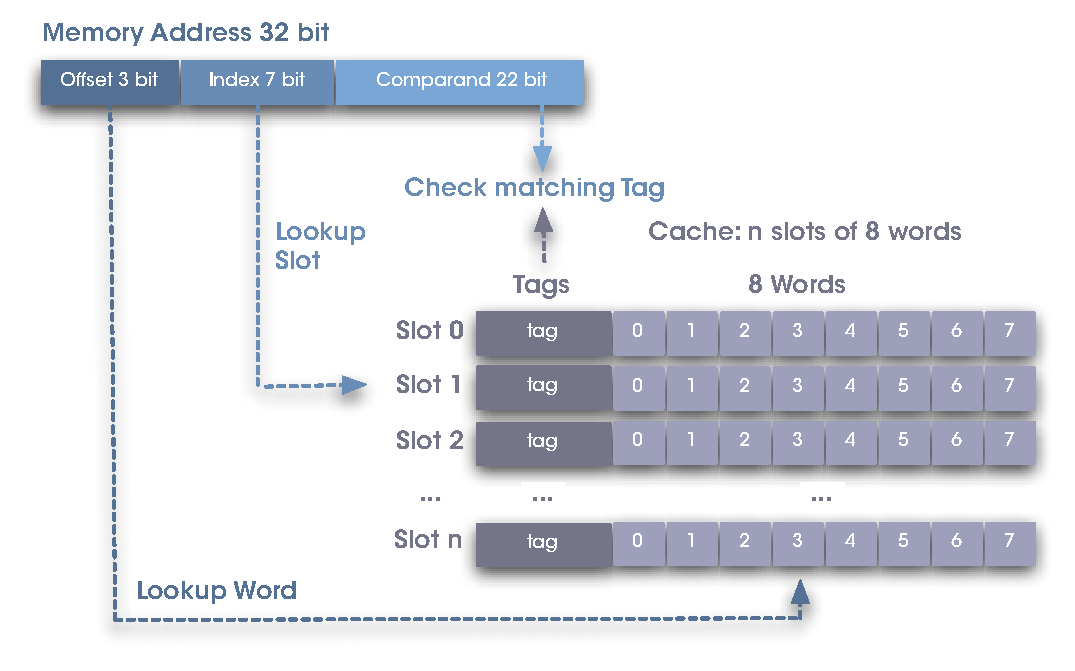
\includegraphics[width=\textwidth]{diagramme/dm_cache}
\caption{Direct mapped cache}
\label{fig:dm_cache}
\end{figure}

The memory address is divided up into three fields. First of all the tag field
which is needed to check if a particular block of main memory is in the cache,
next the index field which will be used to lookup up a particular slot in the
cache and last the offset field which is used to identify a particular memory
word.

When a block of main memory is stored into the cache, the tag field is stored
as a reference for future access in the appropriate slot of the cache. A second
access would reveal that the tag field matches the tag in the cache and the
current block is present in that particular slot. The offset field would
identify the word needed within the slot. The result would be a cache hit
otherwise a cache miss.

The order of the tag and slot fields is important. If they were swapped,
adjacent blocks of memory will mapped to the same slot. As mentioned before
most programs work on the data in close proximity by the means of spatial
locality (see above). That means that blocks which lie nearby would
be swapped in and out of the cache \cite{Harman04}.

\subsubsection{Direct Mapped Cache Example}
For further considerations and illustrations the following assumptions will be
made. The addresses are 32 bit long, the cache itself has 128 slots and 8 words
per slot can be saved. The total cache size would be
$128\ slots\ *\ 8\ words\ * 4\ byte = 4K$.
To clarify the picture of splitting the address into fields the figure
\ref{fig:addsplit_dmc} shows a layout of a address.

\begin{figure}[H]
\centering
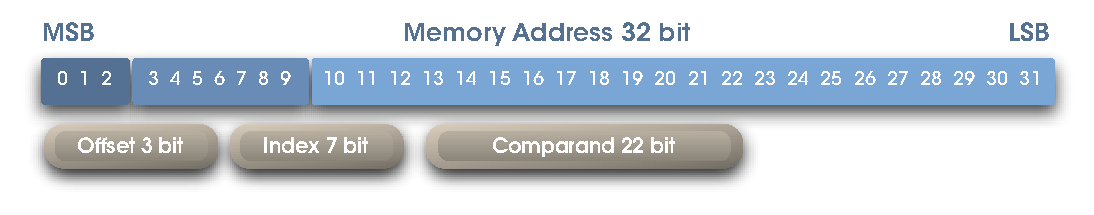
\includegraphics[width=\textwidth]{diagramme/addsplit_dmc}
\caption{Address layout for a direct mapped cache}
\label{fig:addsplit_dmc}
\end{figure}

To identify the word inside the cache line the last 3 bits of the address are
used. A cache with 128 slots needs 7 bits to address the right slot in the
cache. The remaining 22 bits are used as comparands and form the tag field.

\subsection{Fully Associative Cache}
The simplicity of the direct mapped cache is the main advantage of that
approach. The disadvantage is its inflexibility when two commonly used blocks
clash\footnote{Clashing means that two seperate blocks of main memory are mapped
to the same slot} and are swapped in and out due to excessive access. The direct
mapped cache is one of the extrema in cache design cause it allows only one
block to be mapped to one slot. The other extrema is the fully associative
cache.

Any block of memory can be mapped to any slot of the cache. The
relationship can be described as $1:m$. Since  any block can be mapped to any slot
 there is no need for slots hence have not to be addressed. Almost the complete
address can be used for the tag field.

Only the first 3 bits are needed to identify the word within the
cache line. Fully associative caches are very flexible but slow because to check
a tag all cache slots have to be searched simultaneously.

As an example we use the same cache layout as before. The figure
\ref{fig:addsplit_fa} illustrates the splitting of the address.

\begin{figure}[H]
\centering
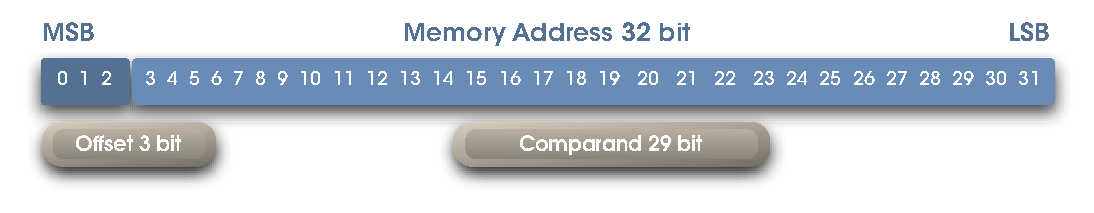
\includegraphics[width=\textwidth]{diagramme/addsplit_fa}
\caption{Address layout for a fully associative cache}
\label{fig:addsplit_fa}
\end{figure}



\begin{figure}[H]
\centering
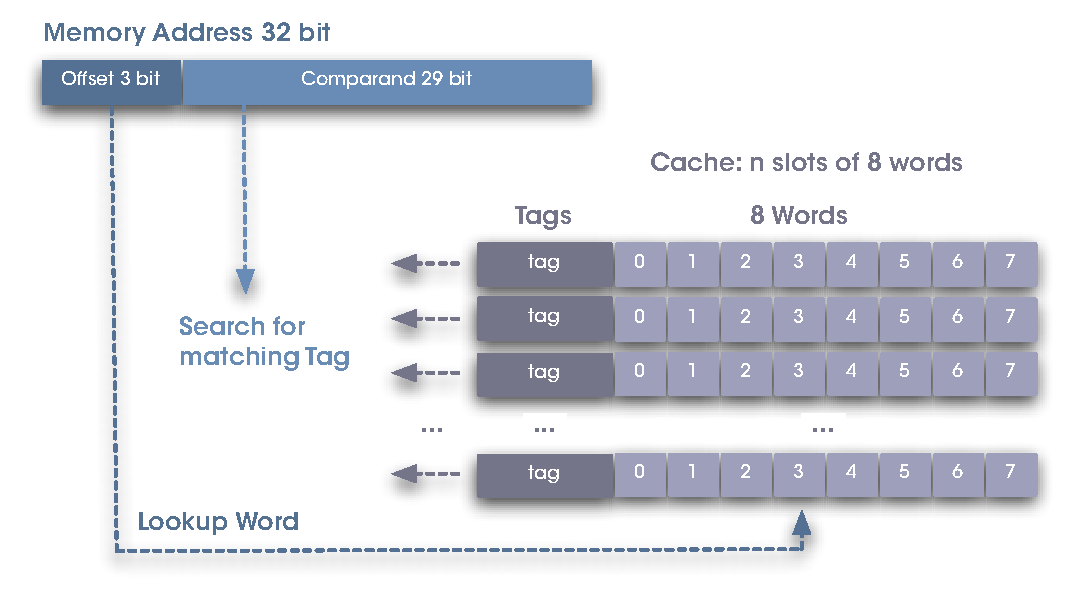
\includegraphics[width=\textwidth]{diagramme/fa_cache}
\caption{Fully associative cache}
\label{fig:fa_cache}
\end{figure}


\subsection{N-Way Set Associative Cache}
The generalization of the direct mapped and fully associative cache is the N-Way
Set Associative Cache. The direct mapped and the fully associative cache are
just special cases:
\begin{description}
\item[Direct Mapped Cache] corresponds to 1-Way Set Associative Cache.
\item[Fully Associative Cache] corresponds to N-Way Set Associative Cache.
\end{description}
Each block of memory is mapped to a small set of slots of cache.
Typically the set size is 2 or 4 and accordingly to the count of slots per set
the mapping is called 2 or 4-Way Set-Associative mapping. The cache is divided
into a number of smaller caches depending to the associativity. Each of these
caches can now store the block from main memory.

The advantage of a Set-Associative cache is that it is flexible and
efficient. The flexibility results by the use of sets, clashes can be avoided as
mentioned before a block can be stored in any of the slots in a set. If a set is
full a cache replacement policy can be applied and space for a new block can be
made.

Instead of searching every slot in the cache only the slots in a set are
evaluated for the corresponding tag. The outcome of this is a higher efficency
compared to the brute force method used by the fully associative
cache.

The figure \ref{fig:addsplit_nfa} illustrates a 4-Way Set-Associative Cache an
d the splitting of the address into the corresponding fields.

The last 3 bits, offset, are used for identifying the word within the cache
line, next 7 bits for set lookup and the remaining form the tag field.

\begin{figure}[H]
\centering
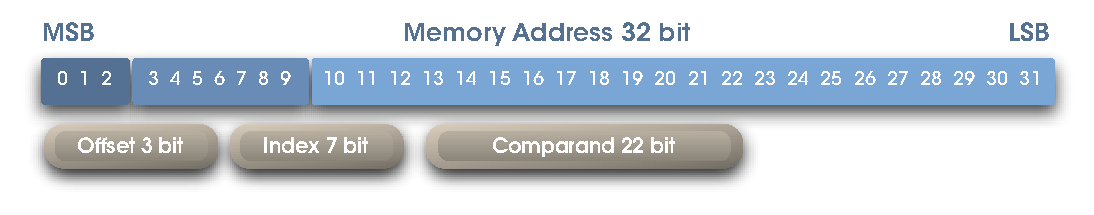
\includegraphics[width=\textwidth]{diagramme/addsplit_nfa}
\caption{Address layout for a N-way set associative cache}
\label{fig:addsplit_nfa}
\end{figure}

The Set-Associative Caches are widespread in practice.

\subsection{Comparison of Cache Mapping Techniques}
\label{sec:comparison_dmc}
There are two simple metrics that show how efficient a cache is. The first is
the hit ratio. The hit ratio describes the likelihood that the cache containing
the memory addresses that the processor requests. An increased hit ratio means
the processor takes full advantage of the cache, a decreased hit ratio results
in many cache misses and the benefit of caching is lost.

The second value is the search speed. If an address is given the cache
mechanism should be able to determine as quickly as possible if there is a cache
hit or cache miss. As in the decreased Hit Ratio case the benefit of caching is
lost if the search is taking too long.

Looking at the \textbf{Direct Mapped Cache} as the simplest of the three types,
it has introduced the easiest check for a hit. Since there is only one
possible place that any block of main memory can be cached there is no need to
search. The cache line either contains the block or not. In the worst scenario
the hit ratio of the Direct Mapped Cache can have a value of 0\%. Consider the
following situation, the processor requests a block A and caches it for future
access, after a while it requests a block B which shares the same slot as A , A
is swapped out and B is swapped in the cache. Now put a loop around it and the
conflict is perfect. The constructed situation has an hit ratio of 0\%. In
general the performance of a Direct Mapped Cache is worst for this kind of
mapping.

The \textbf{Fully Associative Cache} has the best hit ratio because any block
from main memory can be mapped to any slot. If a slot is full the next free slot
is taken cause there is no dedicated slot the cache must use. As beformentioned
the Full Associative and Direct Mapped Caches are two opposite extremas. The
Direct Mapped Cache suffers from Hit Ratio failure and as an opposite the Fully
Associative Cache lacks of performance in searching the cache. A given address
can be stored in any of the slots therefore the search must probe every slot
for a cache hit respectively cache miss. This extra search adds cost, complexity
and execution time.

The \textbf{N-Way Associative Cache} is a good compromise between the other two
cache mapping techniques. Considering the example above and supposing a 4-Way
Set Associative Cache the given address can be stored in 4 places within a set.
The address as described above would now map to the same set and not to the
same slot. The hit ratio has risen \textit{dramatically} form 0\% to 100\%, of
course this is a very simple example but it shows the advantage of the Set
Associative Caches. In a set there are only 4 slots to examine, hence searching
is not very complicated, but adds a small amount of execution time.

To sum up here is a short listing with a comparison of the cache mapping
techniques.
\subsubsection*{Direct Mapped Cache}
\begin{description}
\item[Hit Ratio:] Good, worst case 0\% if two addresse share the same slot
\item[Search Speed:] Best, every address has a dedicated slot, address is
retrieved instantly
\end{description}

\subsubsection*{Fully Associative Cache}
\begin{description}
\item[Hit Ratio:] Best, very flexible an address mapped to any slot
\item[Search Speed:] Moderate, every slot has to be examined whether cache miss
or cache hit
\end{description}

\subsubsection*{N-Way Set Associative Cache}
\begin{description}
\item[Hit Ratio:] Very good, very flexible an address mapped to any slot in a
set
\item[Search Speed:] Good, only the slots in a set have to be examined
\end{description}

There is another aspect of the N-Way Set Associative Caches. If N increases and
hence the associativity is higher, the search speed will become worse as there
are more slots in a set to be examined and the hit ratio increases in the wake of
additionally slots in a set.

\subsection{Writing and Replacement Policies}
\label{sec:wrrdpolicies}
An occuring memory write to a word in cache occurs, the new information can be
written into the main memory immediately or it can be written when the changed
block is thrown out of the cache. The first technique is called write through and
the second write back. The second is more efficient but can complicate things if
the block is needed by several threads or CPU's. The block in the cache and main
memory can become inconsistent and as a result the inconsitency is carried
through the calculation to the point of writing the calculated result back into
main memory.

Another point to consider is what to do if all slots are occupied. How
does the cache decides which of the address to dicard. In a Direct Mapped Cache
the decision is straightforward cause there is no choice. In other mappings the
cache has to take care of it.
The three most commonly used algorithms are \textit{Least Recently Used (LRU)},
\textit{First in First out (FIFO)} and \textit{random}. Because of the increasing
cost to implement true LRU as the set size increases, pseudo LRU or random
replacement policies are sometimes used in practise \cite{Hennesy96}. The
performance penalty of using a random, in fact pseudo-random replacement policy
is very small and it is very easy to implement.

\subsection{Demand Analysis for a Cache in the Ray Tracing Engine}
\label{sec:demand_analysis}

The SPU operates directly on instructions and data from its dedicated local
store, but relies on a channel interface to access the main memory and other
local stores. The developer is responsible of fetching data at the right place
and in the right time into the local store for computation. This means
everytime when the SPUs have to access data from main memory first of all data
has to be fetched into the local store and after processing the results have to
be written back into main memory.

This seems like too much overhead when dealing with programmability of the SPUs
but with the lack of an automatism the developer has a much finer granularity
in programming memory access and can easier and effective exploit the memory
access.

This advantage has a another side, too. The SPUs have no hardware cache and
hence lack of support for caching. Everytime when data is not available in the
local store the computation stops until the desired data is fetched and
available. Of course the data has to be written back if other SPUs rely on the
result.

How this difficulty affects the workflow of the ray tracing process and
which steps has to be taken will be examined in the following section.

\subsubsection*{Caching of Crucial Data}
The big advantage of choosing the shared memory programming model is that the
complete ray tracing process in the SPUs is completely decoupled from the other
SPEs and the PPE. The DMA access from one SPE does not interfere with other SPEs
because there is a fixed assignment of an SPE to a specific tile and results can be
written independently into the main memory. The needed data for rendering the
frame are fetched read only from global structures and hence no problem of
concurrency will arise.

To render a frame each SPU needs a replica of the scene in the local store.
The complete scene consists of different objects with their specific material
properties and light sources. Simple scenes could be fetched as a whole into the
local store, but a big complex scene with several thousands of objects raise a problem.

Therefore it is substantial to develop a clever strategy which assures that data
is in the right time at the right place.

Furthermore the objects are organized into lists which are assigned to specific
voxels which built up the grid (see \ref{sec:rt_design}). The obstacle which arises
here is that first the lists have to be fetched into the local store and then the
objects. Which objects have to be fetched is stored in the lists of the specific voxel.
The ray tracer operates firstly on voxels and not on every single object. It is clear
that the grid lists has to be replicated along the SPEs, too.

With the knowledge which data has to be fetched now a closer look at the
program flow has to be taken for determining how often each data is accessed.
Data which is accessed only one time is not considered because one time fetched
the data resides in the SPUs local store until the end of rendering. Such data would
be the display dimension, angle of view and pixel aspect ratio.

To clear the picture a little bit the following sections will show pseudo code
of procedures which access the main memory frequently.

\lstset{escapeinside={(*@}{@*)}}
\subsubsection*{I. Find Closest Intersection }
\begin{lstlisting}[caption=Pseudo code for "find closest intersection"
function]
procedure find_closes_intersection
begin
	...

	while(1)
	begin

		get_object_list(current_voxel);(*@\label{l:voxel_list}@*)

		while(objects_in_list)
		begin
			intersect_object_with_ray(object,ray);(*@\label{l:ob}@*)
		end;

		if (intersects)
		begin
			break;
		end

		traverse_to_next_voxel();
	end;

	...
end;
\end{lstlisting}

The \textit{find closest intersection} function is responsible for finding the
closest intersection between the actual ray and the objects contained in the
scene. It utilizes the space subdivisoning scheme to traverse fast through
the grid.  For the fast traversal every voxel with its assigned objects is needed.
During the traversal intersection tests are performed. For these the objects
and the ray is needed.

Looking at the pseudo code it can be seen that first of all the object lists
have to be fetched from main memory into the local store as seen at line
\ref{l:voxel_list}. While there are objects in the current list intersection tests in line \ref{l:ob} are performed with the current object and the ray. Since objects are
also located in the main memory they have to be fetched into local store, too.
How often intersection tests are performed depends on the object count in the
lists. The objects are inhomogenously spread along the voxels and hence the
 count of objects can vary drastically. The count of the lists which is equal to the count of voxels in the grid is normally static and assigned at programming time.

During ray tracing the rays traverse through all voxels and intersect all objects.
In the worst case rays leave the grid and do not intersect any object nevertheless
intersection tests are perfromed at every voxel and object lists and
objects are fetched from main memory. On the other side it happens that voxels which
are traversed are completely empty and hence no access to main memory is needed.

Assuming a frame with the dimension 640x480 which makes 640 * 480 = 307200
rays it follows that for each ray 307200 times the corresponding object lists and
objects contained in the list have to be fetched from main memory. This example with
relatively small dimensions shows the big amount of rays which have to be processed.
This number can be drastically reduced if the access patterns are observed and
recognized as the rays are used successive and in an iterative manner.

Nearby rays will probably traverse the same voxel and intersect the same objects, see
section coherence \ref{sec:coherence}, hence the same object lists and objects will
be fetched into the local store. Considering also the big amount of rays it is clear
that many accesses to main memory can be avoided if the needed data is kept in the
local store as long as possible for future use. If the scene uses big objects it is
clear that  more rays will intersect these specific objects and the coherence
can be exploited at a higher degree.

A further consideration is the rising number of objects in complex scenes. Scenes are
often composed with hundreds of objects hence the count of memory  accesses increases
drastically with more complex scenes if the data is not cached.\\
\subsubsection*{II. Shade Pixel}
\begin{lstlisting}[caption=Pseudo code for "shade pixel"
function]
procedure shade_pixel
begin
	...

	for i := first_light to last_light do(*@\label{l:lights}@*)
	begin
		diffuse_light(object_material,normal);(*@\label{l:mat}@*)
		specular_light(object_material, normal);
		transmissive_light(object_material, normal);
	end;

	...
end;
\end{lstlisting}

The \textit{shade pixel} function shades a pixel for each light source in the
scene. The corresponding values are calculated with material properties of the
objects and lights.

The first objects that have to be fetched are the lights. If the lights don't
change between consecutive frames, they can fetched once and stored in the
local store. Normally there are not many lights and they are at fixed points.

For each light as shown in line \ref{l:lights} the objects material and the
actual ray is needed to compute the resulting color, hence the material
properties of each object that is intersected by a ray has to be fetched
 from main memory.

It is incidental that with an increasing number of objects the
amount of memory accesses increases dramatically with more complex scenes as
shown in the previous section. Furthermore the consideration about
spatial coherence apply here as well as they applied in the previous section and
the material data should also be kept in the local store as long as
possible.\\\\
To sum up which data each SPE needs and how often this data is accessed shows
the following list:
\begin{description}
\item[Object lists:] Worst case: for every ray and for every traversed voxel,
Average case: for every ray and voxel containing a hit
\item[Objects:] Worst case: for every ray and every object list, Average case:
for every ray and the resulting object lists from the traversed voxels
\item[Material:] Worst case: for every pixel, Average case: for every hit
\item[Light sources:] Worst case: per frame, Average case: once
\end{description}

It is apparent that there is a big amount of memory accesses considering the
whole chain from casting the ray to the caculation of the color. Taking the
worst case to calculate actually only one pixel, every object list, all objects
contained in the list, every material corresponding to the objects and light
sources have to be fetched into the local store. Considering now an image with
a dimension of $640x480$ pixels, $3000$ objects result in
$640 * 480 * 3000 = 9 * 10^9$ memory accesses. This is of course a simple
and extreme example but it shows the complexity of ray tracing when programmed
in the naive approach and without acceleration techniques.

\subsubsection*{Conclusions}
For the new ray tracer a cache will be implemented. The cache will store all
crucial data which is often accessed and needed for computation. As seen in the
previous sections it is important to cache the object lists, the objects
itself, material properties and the light sources. We can take great advantage
of caching because nearby rays will use the same data and thus the spatial
coherence can be exploited. Therefore a 4-Way Set associative cache will
used in the application architecture. Firstly because that way the SIMD unit is
fully exploited. Secondly the overhead of searching in a set is diminished as
the SIMD unit can handle up to 4 integer values and process them with one
instruction.

Why caching will work for the ray tracer on the Cell BE will be explained
in the following section.

Locality of reference
describes the fact that most data fields that  are in close proximity to each
other, are accessed over and over. This fact applies perfectly to ray tracing
 as the objects are accessed over and over again.

Furthermore the objects lie in close proximity and are accessed sequentially
which is a fact of sequential locality. Resources like objects, material, light
sources which are referenced at one point in time will be referenced again
sometime in the near future, not later than the next ray, describes the fact of
temporal locality.
Last but not least spatial locality can be easy identified in the ray tracing
process. Ressources are likely to be accessed by the next iteration  respectively
by the next ray if a resource nearby was just referenced this fact is known as
spatial locality.

The principle of locality applies perfectly to ray
tracing and is the reason why caching works and will be a remedial action to
improve performance.

The access to the memory will be dramatically reduced with the presence of a
cache. The CPU has to wait for memory far less often than it otherwise would.
In the case of waiting for memory the CPU can do its work and the cache takes
care of fetching data from memory.


\section{Load Balancing}
\label{sec:analysis_load_balancing}
Workload of parallel applications have a dynamic character and can change
during runtime. For a efficient use of a parallel system the workload has to be
balanced between the nodes. Load balancing is essential task for the efficiency
of a parallel system.

A large number of applications partition their workload into a subworkload which
is then distributed to the nodes. How this partitioning is done depends on the
algorithm and on the property how the workload can be subdivided. For example
in the context of ray tracing such a subworkload can be a single pixel, ray,
ray packet, tile or a whole image if we are rendering animations. As the
computation proceeds it comes out that some nodes are faster with
their workload and some are slower as due to the difference in the complexity
off the subworkloads. This imbalance is a major cause of performance losses.

This imbalance can appear multiple times during execution, therefore the
balancing scheme itself has to be highly efficient in order to ensure an
overall benefit otherwise too much time would be wasted on calculating the
balanced state and the effort would have diminishing results.

The workload has to be divisible and it has to be possible to migrate parts of
the workload from one node to another. How this is done depends on the workload
and the communication facilities of the parallel system.

A common approach is based on a 2 phase model. The first phase includes the
calculation of the current workload and the amount of workload which has to be
distributed to achieve a balanced state. The second phase, the
scheduling, includes the migration of workload to the corresponding node
according to the calculations from phase 1 \cite{Elsaesser98}.
There exist other approaches which split these two phases further apart but
these new phases just describe substeps of the general two phases.

\subsubsection*{Requirements for Load Balancing Schemes}
To calculate the flow of workloads for a balanced state the actual calculation
has to be stopped, therefore the determination of the workload flow has to be
highly efficient. A second requirement is that the amount of migrated
workload is as small as possible. It happens that workload is
circular redistributed if the amount is too big. Furthermore the load balancing
scheme should be numerically stable. Minimizing simultaneously the runtime and
the flow turned out to be impossible \cite{Arndt03}.
Therefore a tradeoff exists between achieving the goal of balancing the workload
and the communication overhead associated to the exchanged load.


\subsection{The Load Balancing Problem}
\label{sec:lbproblem}
In the context of ray tracing the main problem is to distribute the
calculations equally for a set of pixels among the nodes involved.  The cost to
compute individual pixels can vary dramatically. It depends on the complexity
of the scene and the ray tracing algorithm being used. Different surfaces will
scatter different amounts and types of light. Depending on the type of the
light (specular, diffusive and transmittive) the calculation varies in multiple
magnitudes.

The time to render an image without load balancing in a parallel
system is the elapsed rendering time of the slowest node in the system, all
nodes contribute a specific set of pixels or tiles to the image.

Tiling an image is essential regarding to the distribution of workload as in
ray tracing the complexity of a tile is not known at the beginning. Heuristics
could be used to determine an initial complexity of tiles but even a small
movement of the camera can discard the effort spent on calculating these values.
These calculation overhead could even be higher than the actual ray tracing,
therefore the initial tiles are untouched and the work is balanced during the
ray tracing process.

Each composite, a composite can be a set of pixels, tile or even a single
pixel, has a sssociated amount of computation $\omega_i$. The granularity of
a composite depends on the structure and data flow of the algorithm.
Considering a ray tracing algorithm that uses ray packets\footnote{Ray packets
are structures that hold a specific amount of rays that are simultaneously
processed.} it is not advisable to distribute single pixels since a ray packet
generates a pixel packet with  the same amount of pixels as rays. The amount of
the computation can be modelled by the number of floating point operations
required to compute the composite \cite{Heirich96}.
The nodes in a parallel system will be indexed by $j$ and a mapping function
$F(i)\rightarrow j$ will be introduced that assigns each composite to a node.
The objective of the load balancing problem is to find an $F$ to minimize
\begin{center}
$T \equiv max_j \sum_{i \in F^-1(j)} \omega_i$
\end{center}
If the node complete their work in the same amount of time $T$ will be at
minimum. Calculating the amount of computation in the same rate for all $p$
computers leads to a minimum $T$ which occurs at
\begin{center}
$T_{min} = \sum_i \frac{\omega_i}{p}$.
\end{center}
The quality of any $F$ can be measured by the percentage of imbalance that it
produces,
\begin{center}
$\epsilon \equiv \frac{(T - T_{min})}{T_{min}}$.
\end{center}
since an objective function is needed to measure the effectivness of any
candidate solution $F$ to any instance of the load balancing
problem \cite{Heirich198} \cite{Heirich298} \cite{Ghosh98}.

It is commonly accepted that parallel algorithms can be implemented so that
they scale linearly with respect to the number of nodes \cite{Basket93}. In
the best cases a speedup of $p$ can be achieved on $p$ nodes.

To solve the load balancing problem there are two main strategies. On the on
hand there are static and on the other hand dynamic strategies.


The static strategies compute an $F$ prior to the start of calculation and are
not modified while processing. A static strategy would be to compute the
complexity in the image and then to distribute the tiles to each node, the size
would be scaled according to the complexity. To generate a good initial
$F$ they can expend considerable amount of resources. The generated $F$ is
vulnerable to data imbalances that arise during processing. An imbalance can
e.g. arise if a tile has only specular surfaces and the remaining only diffuse
surfaces. The calculation cost per pixel on specular surfaces rises multiple
times cause additional rays are generated and have to be traced.

Dynamic load balancing strategies work during the course of calculation to
redistribute the work to the nodes. There are two major algorithms in the
context of dynamic load balancing. They both work locally, require no global
communication and expend computational work only in areas where it is needed.
They diverge in the model of communication between the nodes. The
\textit{diffusion} algorithms assume an all-port-communication model which
 means that each node has a communication channel to any other node. The second
 algorithm the
dimension exchange method, assumes an n-port-communication model which handles
cases where not all nodes are reacheable.

With the dimension exchange method, a node goes around the \textit{table},
balancing workload with its nearest neighbors one at a time. With the diffusion
method, a processor communicates simultaneously with all its nearest neighbors
in order to reach a local balance.

Demonstrations of diffusion algorithms showed that they are a general solution
to the problem of load balancing and have the properties as beformentioned
\cite{Cybenko89} \cite{Dijkstra80}. An advantage of diffusion algorithms is
that they converge at rates that are independent of problem scale
\cite{Heirich95} \cite{Heirich97}.

\subsubsection*{System Model and System Graphs}
The most load balancing methods rely on a model of the underlying system. The
model often used is similar to the models in \cite{Cybenko89} and
\cite{Hosseini90}. The model describes a system composed of a finite set of
autonomous, homogeneous nodes connected by a point-to-point communication
network. How this network works or is built up doesn't matter hence not
specified. Each node has a number of bidirectional communication links
through which the nodes interact synchronosuly with its neighbors.

The system that consists of the nodes and its communication channels
can be depicted as a simple graph $G = (V, E)$, where $V$ is a set of vertices
labeled from $0$ to $n-1$  and $E \subseteq V \times V$ is a set of edges.
Each vertex represents a node and each edge $(i, j) \in E$ represents a
communication link between processor $i$ and $j$. The figure \ref{fig:system_graphs}
shows examples for system graphs.

\begin{figure}[H]
\centering
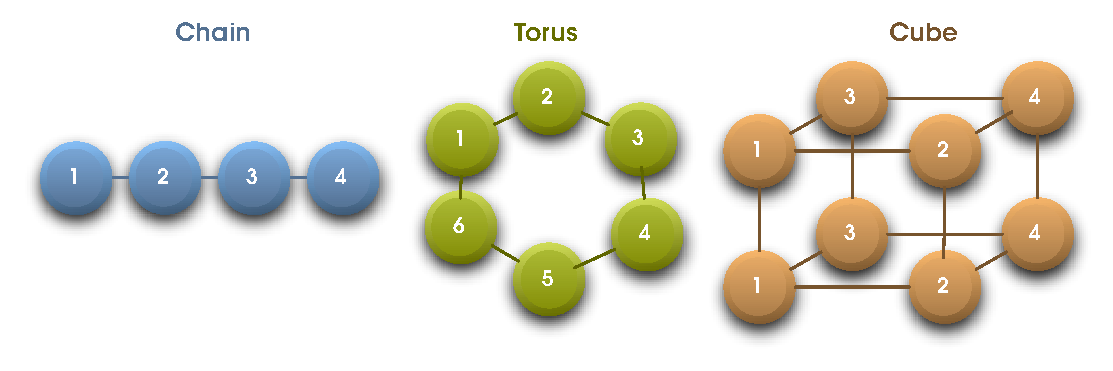
\includegraphics[width=0.8\textwidth]{diagramme/system_graphs}
\caption{Various system graphs}
\label{fig:system_graphs}
\end{figure}

The underlying computation is assumed to comprise a large number of independent
processes. The basic unit of workload is a process, and one or more processes
may be running in a node at any time.

During the period of computation no processes are killed or created. The total
workload in an instance of load balancing is assumed fixed \cite{Hosseini90}
\cite{Xu92}.


\subsection{Dynamic Load Balancing by Diffusion}
A good load balancing scheme is characterized by the ability of scalability.
The cost of an algorithm should be in proportion to the number of computers.
Diffusion is one of the few load balancing schemes, besides dimension exchange
that is provably scalable \cite{Heirich198}. Other problems in placement and
partitioning, like the mapping problem, are solved with diffusion algorithms.
They provide scalable solutions to often encounterd problems in parallel
systems.

The next section will present the First Order Scheme diffusion method (FOS). The
FOS belongs to the family of diffusion methods and was developed by Cybenko
 \cite{Cybenko89}.
The diffusion method was soonly picked up and faster diffusion methods were
introduced \cite{Muthu96}.  These algorithms are faster and have a higher
 convergence rate. For an in-depth analysis of diffusion methods see
\cite{Cybenko89} \cite{Diekmann99} \cite{Diekmann97} \cite{Elsaesser99}.


\subsubsection{First Order Scheme}
The FOS method is the first and easiest diffusion method and works as follows.
Each processor $p_i$ compares its current workload $w_i^k$ with each of its
neighbors load in turn and transfers enough work units to achieve a local load
balance. This process is repeated until all nodes detect the load to be
locally balanced.

The diffusion methods do not generally provide a immediatley balanced solution,
the process is iterated until the load difference between any two nodes is smaller
than a specified value.

\subsection{Dynamic Load Balancing by Dimension Exchange}

The difference between the diffusion and dimension exchange methods is the way
how the nodes communicate with each other. The diffusion methods assume a multi-port
communication model, which means that each node has a communication channel to
all other nodes. In the dimension exchange method, load balancing happens in one
dimension at a time, where a dimension corresponds to some subset of all pairs
directly connected nodes. Every dimension would take its turn, and the whole
process repeats until some satisfactory equilibrium is reached \cite{Xu92}. At every
turn the workload is splitted equally to directly connected processors.

The use of this method on hypercubes was analyized by Ranka et al. \cite{Ranka88}
and Cybenko \cite{Cybenko89} and later extended to arbitrary structures using the
technique of edge-coloring of graphs.

For certain structures like the chain, the ring, the mesh, and the torus an equal
splitting does not necessarily lead to an optimal efficiency. The faster the load
balancing method converge to a balanced state the more efficient is the method.
Xu and Lau showed that for some structures, non-equal splitting of
workload between a pair of processors would yield better results. They introduced
the Generalized Dimension Exchange Method with an exchange parameter that characterizes
the splitted workload between a pair of nodes \cite{Xu92}.

\subsubsection{Generalized Dimension Exchange}
The Generalized Dimension Exchange (GDE) method operates on color graphs derived from
edge-coloring of the given \textit{system graphs}. The \textit{system graph} is
the simple connected graph of the given structure that can be an arbitrary shape
(chain, ring, hypercube, cube...).

For the  description of the Generalized Dimension
Exchange method a system graph $G = (V,\ E)$ with a shape of a cube is assumed.
By edge-coloring \cite{Fiorini78}, the edges of $G$ are colored with some minimum
number of colors $k$ such that no two adjoining edges are of the same color.
A \textit{dimension} is then defined to be the collection of all edges of the
same color. A k-color graph is therefore k-dimensional and load balancing
in the Dimension Exchange as well as in the GDE method happens in one dimension
 at  a time. The minimum number of colors $k$ is strictly bound by $\delta(G)$
denotes the maximum of the degrees of $G's$ vertices,
and $\delta(G) \leq k \leq \delta(G) + 1$ \cite{Fiorini78}.

The colors for in a given k-color graph are indexed with integers from $1 to k$.
The resulting representation of the system graph can now be described as
$G_k = (V,\ E_k)$, of which $E_k$ is a set of 3-tuples of the form
$(i, j; c), (j, i; c) \in E_k$ if and only if c is the color number of the edge
$(i, j) \in E$. The figure \ref{fig:colored_graphs} shows examples of colored
system graphs.

\begin{figure}[H]
\centering
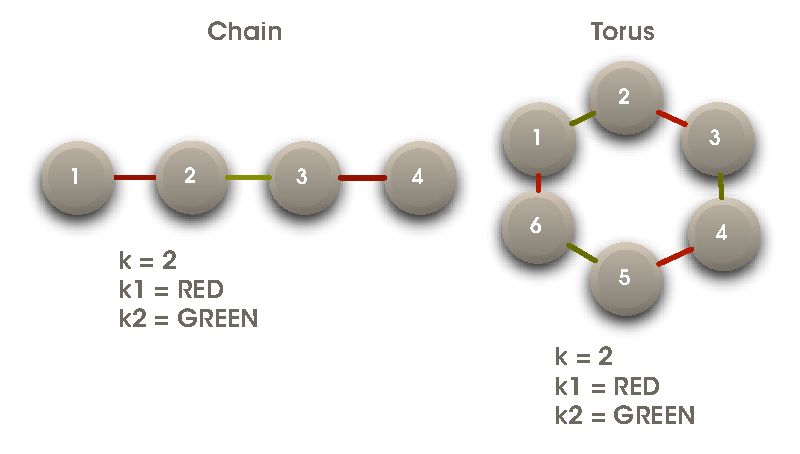
\includegraphics[width=0.6\textwidth]{diagramme/colored_system_graphs}
\caption{Various colored system graphs}
\label{fig:colored_graphs}
\end{figure}

For a given $G_k$ let $w$ denote the current workload of a
node and $\lambda$ denote the exchange parameter chosen for the GDE method. The GDE
method works as follows.

\begin{lstlisting}[caption=Pseudo code for the Generalized Dimension Exchange method]
procedure balance_load
begin
	for i := processor i (0 <= i <= n) to processor n
        begin
                 while(run)
                 begin
                        for c := 1 to c <= k
                        begin
                               if (incident edge colored c) then
                                    inputload = exchange(c);
                                    w = (1 - y) x w + y x inputload;
                        end
                 end
        end
end;
\end{lstlisting}

The algorithm is run each node in a fully decentralized manner, and a node finishes
a complete sweep after $k$ consecutive exchange operations. As such, the node
interact with all of its neighbors one at a time in each sweep. To guarantee that
the workload $w \geq 0$ the exchange parameter $\lambda$ is restricted to $[0,1]$.
If the exchange paramter $\lambda$ is $1/2$ the GDE method is equivalent to the
original dimension exchange method. The exchange parameter is not for forcing a
convergence which is present in the original method but rather improving the
convergence rate.

\subsection{Consideration of Load Balancing Strategies for the Architecture}

Static load balancing strategies partition the image into tiles and distribute them
along the nodes. The different portions, the tiles,  are concurrently rendered and
saved. Such naive strategies that partition contiguous segments of the image fare
poorly  as they suffer from effects of locality in the image which
can lead to wide variations in workload for different nodes \cite{Heirich198}. The
following two sections describe two of the most common strategies used in the context
of ray tracing.

\subsubsection{Pixel Based Scattering}
The pixel based scattering strategy assigns pixels in an alternating sequence
to each node so that $F(i) = (i\ mod\ p)$ where $i$ is the pixel and $p$ is the count
of processors. This strategy is more effective than the naive tile assignment as the
granularity is finer and pixels with similar workload are spread among the
featured nodes.

\subsubsection{Tiling Strategy}
Another  popular static load balancing strategy partitions the image into smaller tiles
 and  randomly distributes them among the nodes. The contiguous regions are now finer
and the random adds a bit of noise to the distribution among the nodes. Analysis showed
that this strategy is less successful than pixel based scattering and the effective
imbalance grows far more rapidly than with the pixel scattering strategy
\cite{Heirich198}.


Nevertheless the tiling strategy will be used in the application architecture. The
combination of the Generalized Dimension Exchange method with the tiling strategy
will extend the static load balancing tiling strategy to a dynamic load balancing
strategy.

The main reason of choosing the tiling strategy is the fact that with pixel based
scattering the posibility of exploiting coherence is not given. Furthermore without
 the coherence which can be easily found in a tile, pixel as well as ray and object
coherence, the performance of the software  cache is decreased as the
pixels are assigned randomly and the ray tracing algorithm is rendering pixels
non-predictable and non-contiguous over a big amount of objects. The very next pixel
is not rendered by the same node but for exploiting coherence
contiguous areas of the images have to be rendered on the same node.


The initial tile should be seen as the initial amount of work and not as the final
workload distribution. When the situation arises that the workload needs to be
balanced, not the whole tile is exchanged but rather ray packets, which represent the
 composite as described in \ref{sec:lbproblem}.\\\\
\textbf{Advantages of this approach}
\begin{description}
\item[\color{Bigblue}{$\triangleright$}] Communication overhead reduced by
  grouping tiles
\item[\color{Bigblue}{$\triangleright$}] Dynamic load balancing is easy, no
  master, each node can
send workload
\item[\color{Bigblue}{$\triangleright$}] The basic approach is easy to implement
  PPE can be
completely decoupled
\item[\color{Bigblue}{$\triangleright$}] Deadlocks no problem, fixed assignment
  SPE - Tile
\end{description}
\textbf{Disadvantages of this approach}
\begin{description}
\item[\color{Bigblue}{$\triangleright$}] Very big scenes tend to be bottlenecks
\item[\color{Bigblue}{$\triangleright$}] Space subdivisioning is not
  parallelizable but can be
done in a preprocessing step
\item[\color{Bigblue}{$\triangleright$}] Most important limitation is memory per
  SPE
\end{description}

\chapter{System Design}
The following sections will show and explain the design of the various parts
of the application architecture. The design is splitted into four parts. The first
part is the ray tracing engine with its algorithmic acceleration techniques
and the interaction between the cache and the load balancer which are the second
and third part.

The fourth part are the Cell programming rules. This is an important part since
the programming rules also effect the algorithmic workflow and data access
patterns. The hardware has obstacles which have to be considered when programming
for the Cell.

Every part is explained first as a standalone part of the application
architecture. After that the view is concetrated onto the architecture and the
interaction between the specific parts.



\section{Ray Tracing Engine}
\label{sec:rt_design}
\label{sec:design_rt}
This section will describe the design of the various parts of the ray tracing
engine. The structure of the sections in the analysis is retained. Each
sub system will be designed and described separately. At the end the interaction
between the various parts is shown.


\subsection{Input Output Handling}
For an easy setup of the graphical output needed to show the result of
the rendering in a window the Simple DirectMedia Layer library will be used.
The library provides a full variety of procedures for window, event, mouse
and keyboard (and more) management.  SDL reconciles all the powerfull libraries
and provides interfaces for each.


\subsubsection{Graphical Output}
\label{sec:design_graph_out}
As stated in section \ref{sec:analysis_graph_out} the SPEs are not capable of
using the procedures provided by the SDL or accessing the surfaces directly.
Therefore a coupling between the PPE and the SPE must be provided. The design of
the graphical sub system will be parted into a PPE part and a SPE part as they
have not much in common looking at the access to the library and the surfaces.

\subsubsection*{The PPE Graphical Subsystem}
The graphical subsystem of the PPE consists of procedures for allocating and
initializing of surfaces and fonts, managing the output window, procedures to
 draw text onto the rendered frame, locking the surface and procedures that blit
one surface into another. The PPE subsystem can be completely written with the
SDL library.

For a flexible setup and use of the SDL library several surfaces are used.
The reason for several surfaces is that each surface can be written independently
and only on demand blitted into the destination surface, the framebuffer. It
doesn't matter if the framebuffer is emulated in software or is available in
hardware the SDL library takes care of it.

The first surface is used for the output in a graphical window. The access is PPE
exclusive which means that the SPEs do not have any handle to access or modify it.
How the graphical window works should not concern the SPEs. The only interface
between the PPE graphical system and SPE graphical system is the second surface.

The second surface is similar to the first the only difference is that the
memory is allocated manually. Firstly to assure that the alignment of the address
is correct, the alignment is crucial for the memory access from the SPEs. Secondly
this way the graphical system of the SPEs knows exactly the dimensions and
writing over boundaries is prevented. Last but not least the surface
allocated by the library is only accessible with library routines which is a big
obstacle for the SPEs.

The last surface is used for the informational output like frames per second,
time needed for rendering and so on. It is just an add-on not a crucial
requirement for the graphical sub system.

A side-effect of using multiple buffers is that double buffering is very easy
implemented. So long as the PPE blits the previous frame of the rendering into
the framebuffer the SPEs are already rendering the next frame in the background.
Double buffering reduces or removes visible artifacts from the drawing process.


\subsubsection{The SPE Graphical Subsystem}
\label{sec:design_graph_out_spe}
In section \ref{sec:analysis_graph_out} it came out that the SPE has to write the
pixels in a specific format into the surface so that the SDL library on the PPE
side can understand and use it. Therefore several auxiliary procedures of the
SDL library are ported to the SPE. These include procedures that map a
3-tuple of Red Green Blue (RGB) values into an integer, that normalize the
3-tuple of RGB values and a procedure that writes pixels into the surface.

The procedures how to map and normalize the RGB values can be looked up in the
source code of the SDL library. There are modified in that way that they use
vectors as the natural data type and make use of SIMD. The last procedure
has to be treated carefully because the ray tracer traces a tile of 4x4 ray
before it is passed to the graphics routine hence the procedure puts a tile
of 4 x 4 integer values into the memory. The rendering of 4 x 4 has an big
advantage as the alignment of the 4th pixel address is always 0xXXXXXX00
(X don't care bits). This is important because the last 4 bits of the local store
memory address and the main memory address must be the same for a successful
transfer. The address where to put the pixel values is fetched from main
memory with various other information.

How the graphical subsystem work together will be shown after the description
of the event facilities as they are needed for synchronisation between frames
and informational input and output between the PPE and SPE. But first of all
an illustration of the graphical subsytem of the PPE and SPE which shows figure
\ref{fig:graphical_subsystem}.

\begin{figure}[H]
\centering
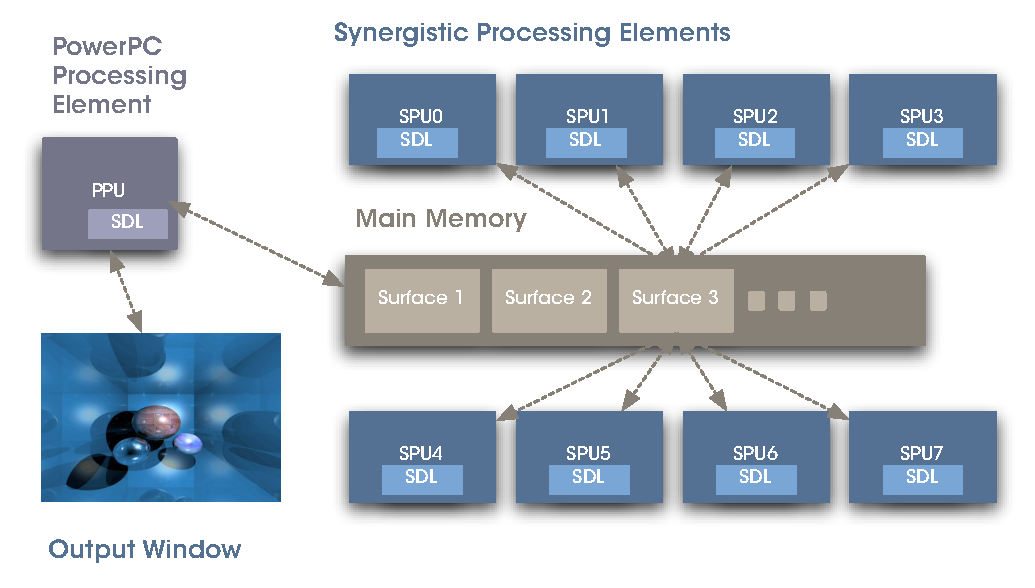
\includegraphics[width=0.9\textwidth]{diagramme/graphical_subsystem}
\caption{The graphical sub system of the PPE and the SPE}
\label{fig:graphical_subsystem}
\end{figure}


\subsection{Event Handling}
\label{sec:design_event_handling}
Events will be used to control the program flow. Each event will be coupled
with an so called event handler that is executed everytime the specific event
occurs.  The event handler will start and stop the ray tracing, move the camera
or synchronize the rendering. Event handling is often used for graphical user
interfaces. For the ray tracer the event handling will also be used for navigation
through the virtual world.

As in section \ref{sec:design_graph_out} this time the event handling is also
split in a PPE part and a SPE part. In the analysis it came out that the SDL library
is providing a sophisticated event handling mechanism that allows an easy setup
for processing mouse and keyboard events. Therefore it is not necessary to develop
a complete new mechanism for the PPE. For the PPE the SDL library will be used.

To merge the events of the PPE and SPE the event facility of the SPE is exploited
and adapted to the events of the PPE.

The next section will explain the SPE event facility.



\subsubsection{SPE Event Handling}
\label{sec:design_spe_event_handling}

For the SPE event handling concepts of graphical user interfaces are used. The actual
representation of the results in a window with which the user interacts can be seen
as an simple user interface.


The event handling framework for the SPE consist mainly of three parts. Firstly
the main event handler that catches all events which occur and delegates the
events to the corresponding handlers. The second part consist of handlers which take
care of the \textit{mailbox}, \textit{signal1} and \textit{signal2} events.
The  \textit{mailbox} , \textit{signal1} and \textit{signal2} are MMIO mapped
registers  which can be accessed through every device which has access to main
memory.
The third part are the procedures which are called from the handlers to process
the signals respectively the messages send through the mailboxes. These procedures
can also be used to send signals and messages to all other SPEs or the PPE. Each
SPE has an handle to the MMIO registers of the other SPE.

What happens if the SPE records an event is the following. First of all
the event handler fetches the event that has occured. After examining the event
the corresponding handler is called. The handler routine first of all masks the
specific event to avoid phantom events (phantom events occur during processing
the current event  and  can not be processed). After extracting the signal
respectively the message the masked event is enabled and again ready for processing.

The figure \ref{fig:event_handling_comp} shows the components of the SPE event
handling framework.

\begin{figure}[H]
\centering
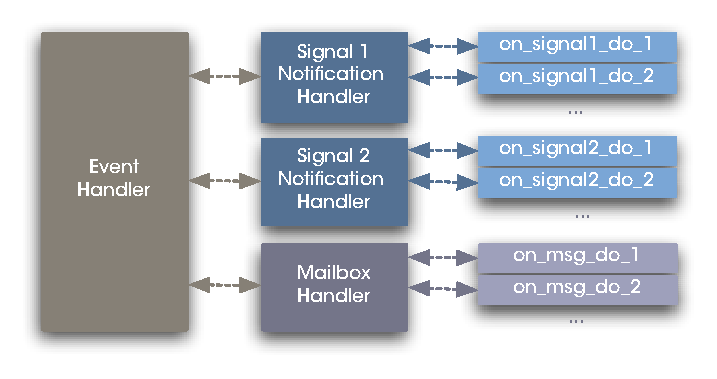
\includegraphics[width=0.6\textwidth]{diagramme/event_handling}
\caption{The Event Handling Components}
\label{fig:event_handling_comp}
\end{figure}


The fact that the SPEs has to signalling channels can be exploited in the following
way. Since the PPE is heavy communicating with the SPE in the case of user
interaction and the SPEs are communication for load balancing with each other it is
advisable to associate all events which come from the PPE with
\textit{signal 1 notification channel}
and all events that come from the SPEs with \textit{signal 2 notification channel}.
In this way
 there is a exact association of events to channels. This becomes handy because
the ray tracer can be split into domains where only one \textit{notification channel}
is active and events of the other channel can be safely ignored.

For example during the rendering of one frame the objects and the camera can not and
are not permitted to change. Hence we assign a domain to that part of the algorithm
and only allow the \textit{signal 2 notification channel} to be active. As we
dissociated the \textit{signal 2 notification channel} from events which accure from
interaction where the \textit{signal 1 notification channel} is responsible for,
there is no chance that any object or camera is changed. But what can
occur are events of the load balancer. These are processed properly and the specific
routines are called.

On the other side if the frame finishes to render and the SPE management procedures
are called  there is no need to balance load. In this phase the frame can be
prepared (camera or object changed) and receive events which occur during
interaction. With the event handling mechanism a fence between two domains of
 an algorithm can be provided to decouple the events that are specific to a domain
of the algorithm.


How the graphical subsystem and the event handling mechanism work together is
explained in section \ref{sec:design_render_frame}.

\subsection{Building the Virtual World}
The description language is based upon the description language of POV-Ray the
free ray tracer. The POV-Ray reference supplies the context-free grammar of the
language which will be used for the compiler.

The compiler will be written with the well known tools Lex and
Yacc. Lex is used for generating the lexical analyzer and Yacc
for generating the parser.

Lex and Yacc are commonly used together. Yacc uses a formal grammar to
parse an input stream, something which Lex cannot do using simple regular
expressions (Lex is limited to simple finite state automata). However,
Yacc cannot read from a simple input stream - it requires a series of tokens.
Lex is often used to provide Yacc with these tokens.

\subsection{Preparing the Frame}
As stated in section \ref{sec:analysis_prepare_frame} for intersection culling
the fast voxel traversal algorithm by \cite{Woo87} is used. The traverse through
the grid the voxels have to be build and the objects to the corresponding voxels
assigned. These actions are the preprocessing steps for the fast voxel
traversal algorithm.

If the user modifies an object by moving or resizing one specific SPE has to be
notified to reprepare the frame. The object is maybe moved farther than the
dimension of a voxel hence the object resides in another voxel and has to be
reassigned. The other problem which arises is that the specific object is
cached and not up to date. To remain coherence between the local store and
main memory the SPE has to tag the specified object as not synchronized
(flag \textit{synchronize} is set in the cache).

With the existing event handling mechanism the synchronisation is easy done
as the PPE can easy send the signal \textit{SYNCHRONIZE} to all SPEs which
than fetch the modified object addresses from main memory and update the cache.

For fully dynamic animation it would be advisable to rebuilt every frame from
scratch and not only the modified objects.

The synchronization of preparing and rendering the frame which has to be considered
separately is also accomplished with events. Each SPE only renders a frame
if a specific signal is recevied. The signals are continously emmited from the PPE.
If the signal do not appear the SPEs are stalled and are waiting for the next
signal. Now the PPE can emit the \textit{PREPARE FRAME} signal and a specific
SPE (which SPE prepares the frame doesn't matter) prepares the frame. Thereupon
the SPE sends the \textit{RENDER FRAME} signal to the other SPEs signalling
the the frame preparation is accomplished. After emitting the signal the SPE which
prepared the frame takes part at the rendering. The computational time which
is needed is remarkably small compared to the rendering time even with frames
with a dimension of 240 x 180 pixels.

Now to the prepare frame algorithm itself. It works like the following.

Since the prepare frame is done on the SPE first of all the objects have to be
fetched. If the count of the object is small enough the whole scene is fetched
into the local store otherwise the objects are multibuffered and only one
buffer at time is processed (double-buffering). This way the memory latencies can
be hidden.

For each object the axis aligned bounding box (AABB) is created. The AABB is
created on demand since they are noly needed for building the grid. The AABB is
described by two vectors. The first specifies the position, the lower left vertex,
and the second vector is the size. Summing the position and the size results in
a vector that specifies the higher right vertex of the AABB.


The easiest way to determine in which voxel an object lies is to intersect
the object with every single voxel. This brute-force method is not really fast
as it depends on the voxel count and on the object count. Another faster method
is to use the AABB of the object to determine in which voxel the AABB may
reside. Now not every voxel is tested only the potential candidates.

With the two vectors the lower left and the higher right it can be determined
where in x, y and z the AABB of the object lies. The x, y and z specify the
coordinates of the voxel in the grid. After intersecting the object
with the voxels the objects address is saved in the list of the corresponding
voxel.

After completting the preparation step the data is ready for taking part
of the rendering process.


\subsection{Rendering the Frame}
\label{sec:design_render_frame}


The ray tracer itself it splitted into three main and two sub modules. The three
main modules are \textit{Render Tiles}, \textit{Render Ray Packet} and
\textit{Raytrace}. The two submodules are \textit{Find Closest Intersection} and
\textit{Shade Pixel} that are used by the main module \textit{Raytrace}. Each of
the modules contributes a specific part to the whole ray tracing process. They can
be seen as parts of a rendering pipeline specifically to the Cell BE ray tracer.

The rendering pipeline with the modules illustrates figure \ref{fig:render_pipeline}.

\begin{figure}[H]
\centering
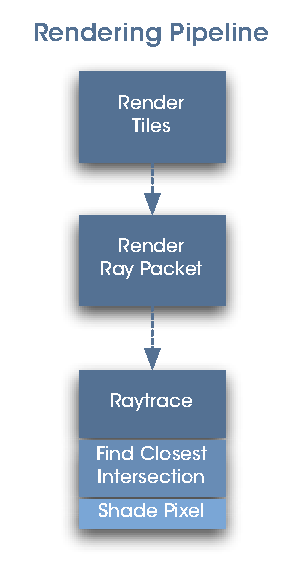
\includegraphics[width=0.25\textwidth]{diagramme/render_pipeline}
\caption{The rendering pipeline of the ray tracer}
\label{fig:render_pipeline}
\end{figure}

The first step before the rendering pipeline becomes active is to initalize
the renderer. In the init step the cache and the loadbalancer are setup.
Furthermore the lights which are needed for shading the pixels are prefetched.
The transfer is initiated and in the module \textit{Shade Pixel} completed.


\subsubsection*{Render Tiles}
\label{sec:design_render_tiles}
The module \textit{Render Tiles} is responsible for rendering the tiles
that are supplied to the SPE. The first step include the calculation of
the eye based coordinate system which is needed  for a distortion free
display of the  rendered scene.  The second step includes the calculation
of the stepping offsets which are used to calculate the direction of
consecutive rays. This is a fast way to calculate the directions as
the dimensions and the pixel aspect ratio included in the offsets and the
module \textit{Render Ray Packet} can calculate the ray directions without
the knowledge of display dimensions and pixel aspect ratio.

The tile is now splitted into regions of 4 x 4 rays and separately processed,
why this step is done is explained in the section of module
\textit{Find Closest Intersection}.
After completting a sub tile the resulting pixels are passed to the
SPE graphical sub system which maps the RGB values and writes the resulting
values into the surface as described in section \ref{sec:design_graph_out_spe}.

The last step includes the examination of pending events.
Section \label{sec:design_event_handling} described that the raytracer is in
another domain in the context of event handling and only responds to signals
which indicate to balance load. If there are pending events the loadbalancer is
activated. After redistribution of workload the ray tracer returns to the management
procedure that is in another domain and waites for signals from the PPE.

\subsubsection{Render Ray Packet}
\label{sec:design_render_ray_packet}
The \textit{Render Ray Packet} prepares the ray packet for ray tracing. With
the offsets from \textit{Render Tiles} the directions are calculated and passed
to the modules \textit{Raytrace}. The last step includes the reorganisation
of the resulting color data for the graphical sub system.


\subsubsection{Raytrace}
\label{sec:design_raytrace}
The \textit{Raytrace} module incorporates the two sub modules \textit{Find Closest
Intersection} and \textit{Shade Pixel}. For every ray in the ray packet the two
modules are called. The main question which arises here is why the rays are
sequentially processed and not kept in the packet. The main reason for this
is that the fast voxel traversal algorithm from its characteristic is very difficult
to parallelize in SIMD. It is not guaranteed that every ray in the ray packet
traverses the same voxels and intersects the same object. Even worse on ray could
pass the whole grid while others intersect objects. It is clear that for one ray
the step into the next voxel has to be performed and for the other ray the
intersection tests, different ray may demand different traversal orders.  The
simplest and fastest way to overcome this is to render each ray in the ray packet
separately and return the rendered packet of colors.

A recently posted article describes a new method of stepping through a grid. The
method is called \textit{Coherent Grid Traversal} that overcomes the problem
of different traversal orders. The method traverses the grid slice by slice rather
than cell by cell \cite{Wald06Grid}. This method is relatively new and the
method is not well documented to be used in this implementation.


\subsubsection{Find Closest Intersection}
\label{sec:design_find_closest_intersection}
The main purpose of the modulue \textit{Find Closest Intersection} is the traversal
of the ray through the grid and performing the intersection tests in the voxels.
The traversal algorithm is based upon the paper \textit{A Fast Voxel Traversal
Algorithm for Ray Tracing} \cite{Woo87}. It works as follows.

The traversal algorithm consist of two phases the initalization and incremental
traversal. The initalization phase begins by identifiying the voxel in which the
ray origin is found. If a ray does not hit the grid hence no objects are hit and
the ray can be discarded. If a ray hits the grid useful parameters are calculated,
given the intersection point of the ray with the first voxel. The X, Y and Z variables
are initialized to the starting voxel coordinates. The X, Y and Z variables are the
coefficients of the canonical grid coordinate system, in which a grid of
$N_x x N_y x N_z$ cell maps to 3D region of $[0..N_x) x [0..N_Y) x [0..N_z)$. In that
coordinate system, the cell coordinates of any 3D point $p$ can be computed simply
by truncating it. In addition, variables for stepping through the grid are calculated
they are initalized depending on the sign of the values x,y and z of the ray direction.

Next values are determined that describe how much along the ray it can be travelled
and still remain in the current voxel. The last variables needed indicate how far
along the ray it must be moved for each component x,y and z to equal the width of
a voxel.

With the current voxel indices and the computed variables the stepping of a ray through
voxels consists basically of two float comparisons and a float add operation
\cite{Woo87}.

In every visited voxel the object list is examined. If there are objects in the
current object list, the ray is intersected with every object. If the closest
intersection is found the traversal is aborted and the point where the ray hits
the object is returned. A major drawback with current space subdivision schemes
is that since objects may reside in more than one voxel, a ray may intersect the
same object many times. Amanatides and Woo suggested a technique called
\textit{Mailboxing}. Every created ray holds a unique \textit{ID} which is saved
along with the intersected object. If the ray traverses to the next voxel
and tries to intersect the same object first of all the \textit{ID} of the ray
and the \textit{ID} of the object are compared. If there are equal the intersection
test is discarded othwerwise the intersection is performed and the \textit{ID}
is again saved with the object intersected.


The module \textit{Find Closest Intersection} is the first module which takes
great advantage of the cache. As the tracing is always performed with ray packets
each with 4 x 4 rays it is likely that each ray will traverse the same voxel
and intersect the same objects. The module caches the object lists and the objects
that are intersected. In the best case where all rays intersect the same object
15 successive memory access can be avoided as the list as well as the object
is in the cache. The first frame will start with a \textit{cold cache} which means
the cache is empty but for successive frames the  cache will be filled which
is also known as a \textit{warm cache}. To exploit the cache the SPE should
render always the same region as randomly hoping would discard the coherence
and the cache had to be updated more frequent than in the other case.

The intersection tests are based upon already well tested algorithms. For the
spheres a geometrical intersection test is used as described in
\cite{Glassner89}. For the triangles the minimum storage intersection test by
\cite{Trumbore97} are used. The tests have an advantage compared to other they do not
require any precomputed values hence no additionally access to main memory
for auxiliary data is needed.

\subsubsection{Shade Pixel}
\label{sec:shade_pixel}
After the closest intersection point is determined and returned it is time
to shade the actual pixel. Given the hit point the surface normal and the vector
towards the light is computated. Now for every light the diffuse, specular and
transmitive light contribution are computed according to the \textit{Hall
Shading Model}. The last step includes the computation of the ambient light.

For every light contribution the material properties of the intersected objects
are needed. Here again great advantage of the cache can be taken. The coherence
and memory acces consideration can also be applied to the module
\textit{Shade Pixel} as in the module \textit{Find Closest Intersection}.

\newpage
\section{Cache Design}

The cache design is heavily based upon the suggestions made in the document
\textit{An introduction to compiling for the Cell Broadband Engine, Part 5:
Managing memory.} \cite{Part5}.

The software cache described for the ray tracer is a 4-Way Set Associative Cache
with 128 bytes
per slot and 512 bytes per set. The use of 128 bytes per slot is due to the fact
that the Element Interconnect Bus (EIB) overhead is minimized if transfers are at
least 128 bytes. Furthermore each variable or data which will be cached does not
exceed the size of 128 bytes. The number of entries is arbitrary and depends
mostly how much space is available in the local store. The footprint of the ray
tracer is about 20Kbytes hence there is enough space to hold 128 or more entries.
With 128 entries the ray tracer could cache 1024 objects, 1024 material properties
or 16K 32-bit addresses.

\label{sec:assoc}
The associativity of 4 is used due to the fact that a set of 4 slots can be
simultaneously examined with SIMD instructions.  The overhead which is given
when searching or comparing each slot sequentially is gone.

The smallest element to be addressed needs to be a word\footnote{Throughout the
whole document a word will have the size of 32-bit}
 because the ray tracer
must be able to cache pointers to specific objects. The object lists consists of
pointers to objects and are not fetched completely. At compile time the list sizes
are not known and each pointer is retrieved separately.

The cache is made up of three arrays. Each array holds specific data needed for
the SPU software cache. The first, the tag array, contains the comparands needed
for the address loookup.  The second, the address array,  contains pointers to
the cache lines and the third contains the cache lines. Each array entry contains
4 slots as is characteristic for a 4-Way Set Associative Cache.

The cache lookup code is inserted at every read reference to a cacheable
variable. As mentioned before in section \ref{sec:cache_analysis} every variable
that is used during ray tracing should be cached. The objects e.g. have an
irregular data access pattern. It is not predictable which objects lie in which
lists hence prefetching is no solution.

The accessed variables are of an arbitrary size and have arbitrary access patterns.
The cache has to deal with and therefore the lookup will be independent of cached data
and access. No matter what is cached the cache will always operate on 128 byte
cache lines. The only thing of which the cache will be aware of is the effective
address of the specified variable. Given the target address the cache returns
always a local store address no matter if the cache encounters a
\textit{cache miss} or \textit{cache hit}.

Various flags which are saved along with the tags represent the state of a
cache line in the cache. The flag \textit{valid} shows that an entry is valid
and can be returned. If data changes in main memory the entries will be flagged
with the \textit{synchronize} flag. If this data is referenced it has to be
reread. In contrast, when the \textit{dirty} flag is set the entries have to be written
back into main memory. Since the SPUs do not modify any cache data, write back
policies are not considered.

The figure \ref{fig:cache_design_rough} shows the overview of the 4-Way Set
Associative Cache for the SPU.

\begin{figure}[H]
\centering
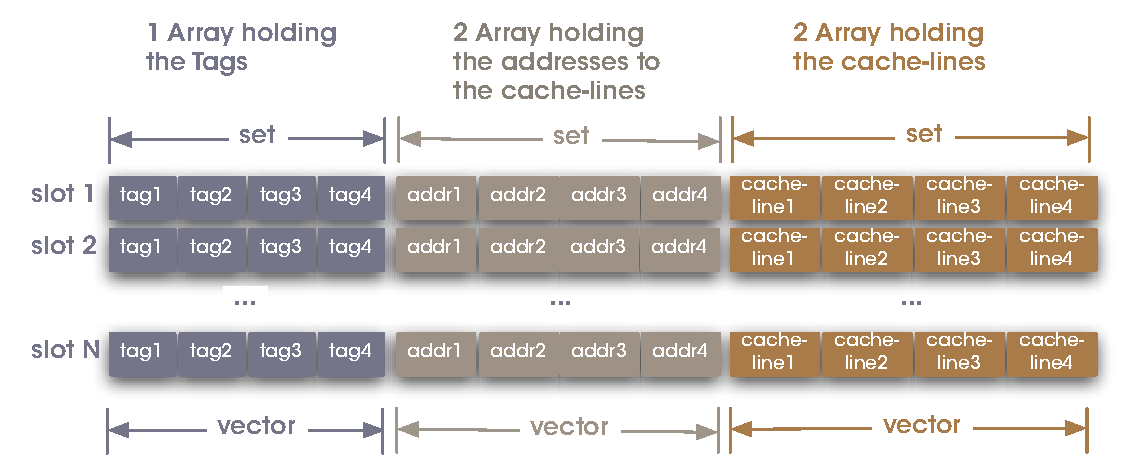
\includegraphics[width=\textwidth]{diagramme/cache_design}
\caption{The design of the 4-Way Set Associative Cache for the SPU}
\label{fig:cache_design_rough}
\end{figure}


\subsection{How the Cache Works}
This section will describe the steps involved to lookup an address in the cache
and the steps to solve specific cirumstances which arise during the cache lookup.
\subsubsection{Cache Lookup}
The cache lookup works as follows. The address from main memory is first
checked with the comparands stored in the tag array at the specific index. The
information at which index to look for the comparands is encoded in the address.
If the comparands match with the given address the cache records a
\textit{cache hit}, the data in question is in the cache and the corresponding
pointer to the data line is retrieved and the offset which is also encoded in
the address is applied. The resulting pointer is returned.

If the requested line is not in the cache, the cache miss handler is called
which is  responsible for retrieveing the specified cache line from
main memory.

\subsubsection{Cache Miss Handler}
The first step of the cache miss handler is to determine if the actual array entry
of tags has free slot. The determination of a free slots in the tag array
determines also the free slot in the address and cache line arrays as they are
interrelated.

The cache find free slot routine checks the array entry and returns on
completion a free slot. If the entry is full a cache replacement policy
is applied. As stated in section \ref{sec:wrrdpolicies} a random scheme is easily
to implement and very efficient. Therefore a random scheme will be implemented
for the SPU cache.

A very simple method to retrieve pseudo random numbers is the linear congruental
method. Linear congruental methods are the oldest and best known pseudo random
number generator methods. They are easyily to implement and fast. As we have only
simple demands this method is adequate. Cryptographic strong pseudo
number generators would be exaggerated.

The pseudo random generator works like this. Given a seed $y$ it calculates pseudo
numbers
according the following function: $y_i^1 = (a * y_i + r)\ mod\ m$. $a,\ r$ are
constant variables which can be choosen randomly. This is not quite true as the
choice of $y, \ r, \ and\ a$ is extremely sensitive, the linear congruental
method is only capable of generating decent pseudo random numbers if these three
values are chosen carefully. Fortunately there exist resources where these
values can be looked up and used for own development. $m$ is the modulus \- in this
case 4 as the entry holds up 4 slots and the cache find free slot routine
should only return values between $0\ and\ 4$.

If the cache find free slot routine determines that a entry is \textit{dirty}
a write back policy has to be called. But since the SPUs do not modify the cached
data the write back policy is unnecessary.

Now with the given free slot the cache miss handler can load the missing data.
After fetching the cache line from main memory first of all the tag and address
entries are updated to ensure that consecutive references of the same address
are found in the cache. The new entries are automatically flagged es being valid
and the requested address of the data line is returned.

The figure \ref{fig:cache_design_flowchart} shows the flowchart of the cache.

\begin{figure}[H]
\centering
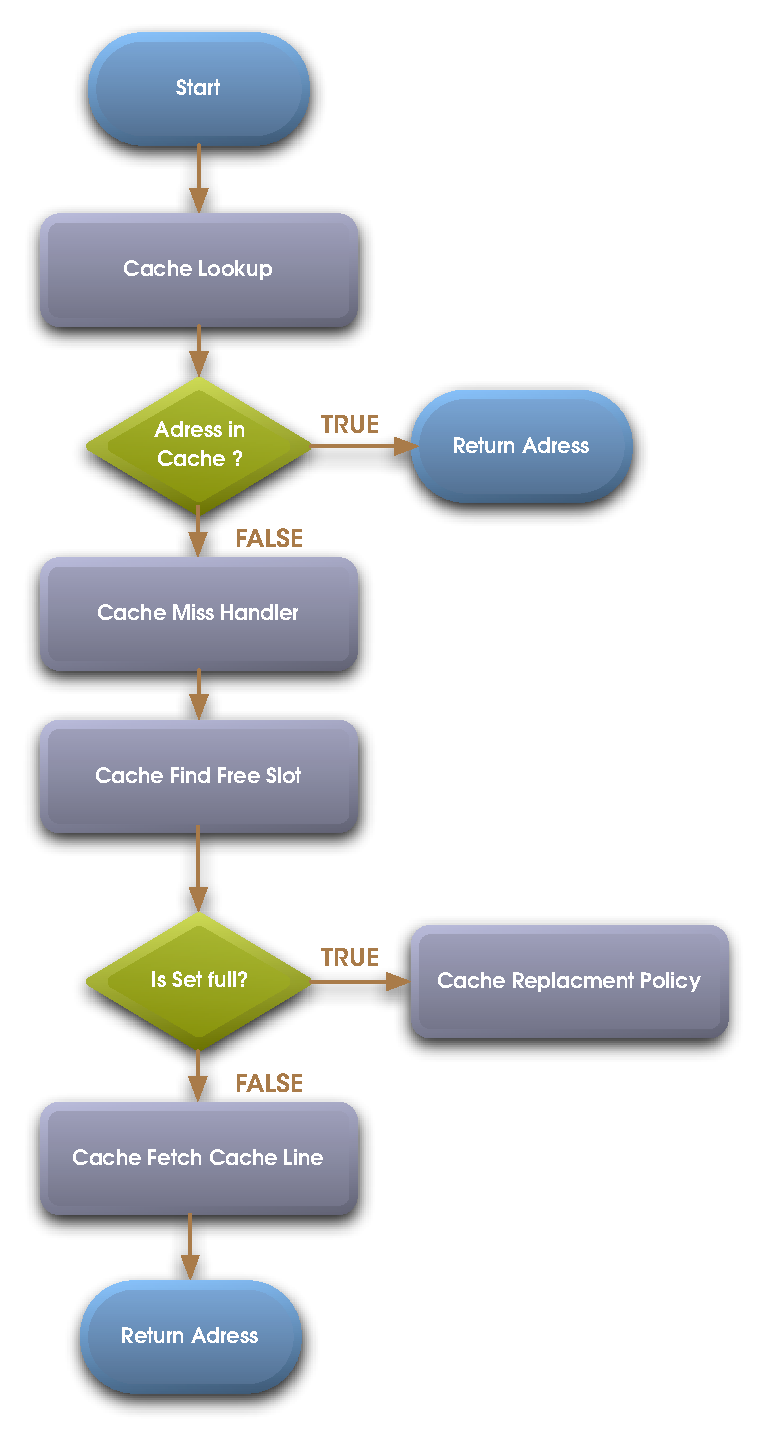
\includegraphics[width=0.47\textwidth]{diagramme/cache_flowchart}
\caption{Flowchart of how the cache works}
\label{fig:cache_design_flowchart}
\end{figure}


Beside other techniques for efficient use of variables stored in main memory like
prefetching and double buffering only the cache has the ability to exploit
locality of reference and reduce access to main memory significantly.


\section{Load Balancer Design}
\label{sec:design_load_balancer}
For the application architecture a sort-first scheme is used, where the screen is partitioned
in disjoint tiles that are rendered by the different nodes (SPEs). The display node (PPE)
is then responsible for receiving the rendered tiles and composing the final image. The
main advantage of such scheme is its relatively small communication requirements. On the
other hand, it is very susceptible to load imbalance \cite{Molnar94}.

The display node (PPE) has to wait for all rendering nodes to conclude their rendering
task before composing the final image. Clearly, the slowest rendering node represents
the bottleneck of the applicatiion so it is crucial to apply a load balancing scheme.

The screen is initially subdivided into a set of N disjoint tiles (horizontal strips),
where N represents the  number of rendering nodes. Each tile is assigned to a SPE hence
there is a fixed assignment between SPE and tile. These horizontal strips build a chain
of tiles which represent the actual image. The tiles or rendering nodes are organized in a chain to obtain the characteristic of the strips. The figure
\ref{fig:tile_assignment} illustrates the tile assignment and the system graph.

\begin{figure}[H]
\centering
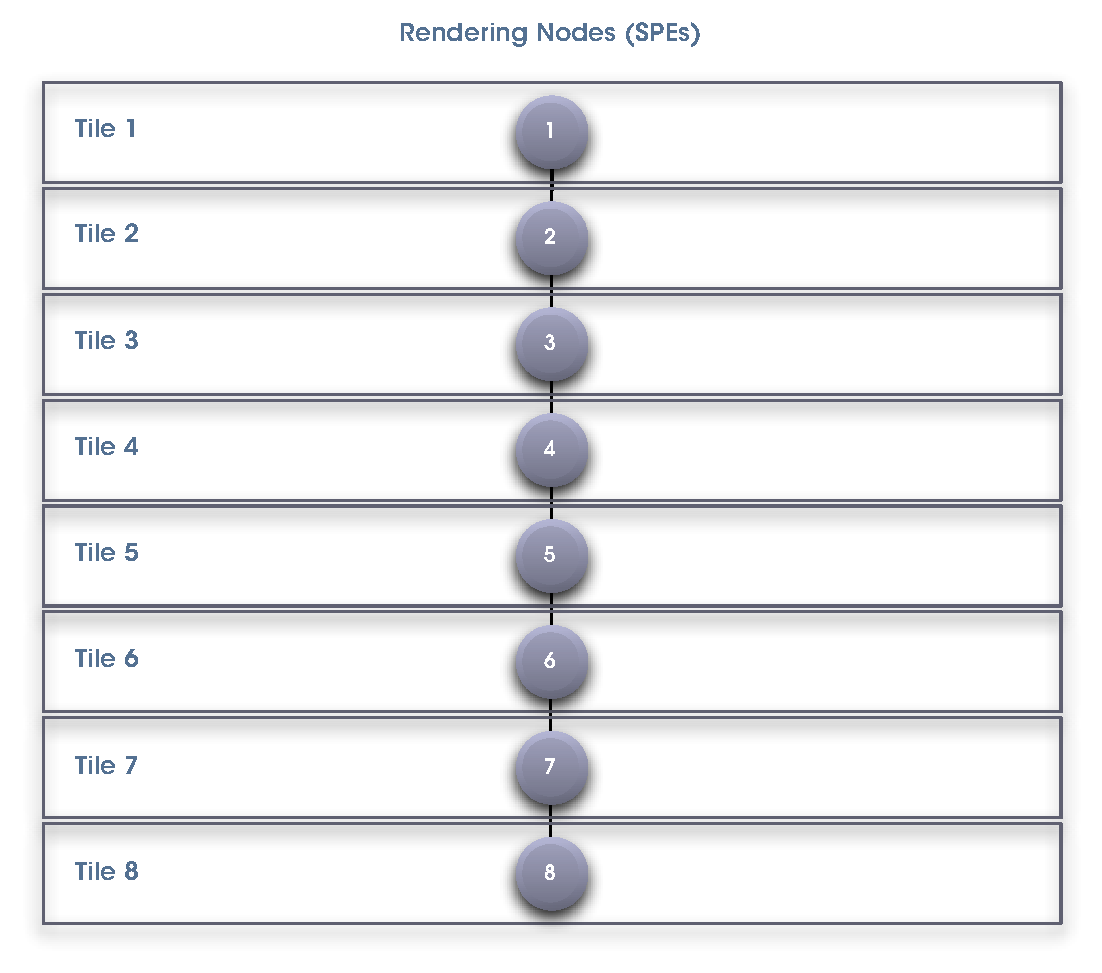
\includegraphics[width=0.6\textwidth]{diagramme/tile_assignment}
\caption{The tile assignment and the resulting system graph}
\label{fig:tile_assignment}
\end{figure}

The algorithm uses the information from the previous frame to adjust the tile sizes in order
to achieve load balancing  for the next frame. Because of frame-to-frame coherence, consecutive
frames have similar load distribution, even for dynamic scenes. The overal effort needed for
rendering one frame is measured by summing the exchanged  workload of all neighbors. The exchange is done by the Generalized Dimension Exchange method which can handle arbitrary system graphs and has a good convergence rate to optimal load balance.

The communication between the nodes is accomplished by the event handling system. Every node
has a handle to its direct neighbor with which the requesting node can send singals or exchange
messages with corresponding nodes.

\subsection{How the Load Balancing Works}
\label{sec:design_how_load_balancing}
When a node gets out of work it sends a signal to its direct neigbors signalling to exchange
workload. As described in \ref{sec:design_spe_event_handling} the load balancing occurs in a
own event domain and is not interfered with other signals that are not concerned to load
balancing. At the same time the requesting node is also sending its remaining workload
to the neighbors via the mailbox. The remaining workload is the count of rows that have to
be rendered.

The corresponding neigbors suspend their computation and send on her part their remaining
workload to the requesting node. At the same time the requesting as well as the
sending nodes gather the workload and process it. The new workload is computated with the Generalized Dimension Exchnage method and the boundaries of the tile are adjusted. Depending
on the position in the chain the higher bound respectively the lower bound has to be adjusted, too. The adjustment is done on every node which is involved
in the current load balancing (in one dimension).

The figure \ref{fig:lb_workflow} illustrates with two adjacent nodes how the workload
is exchanged and the tiles adjusted.

\begin{figure}[H]
\centering
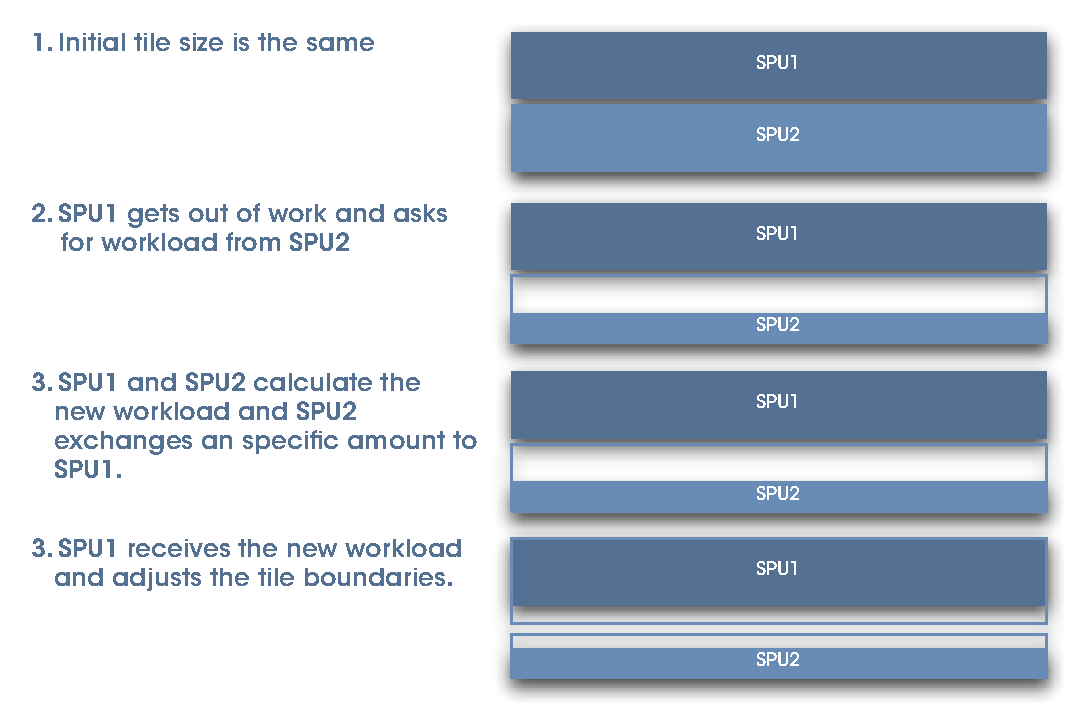
\includegraphics[width=0.8\textwidth]{diagramme/lb_workflow}
\caption{Tile boundaries adjustment}
\label{fig:lb_workflow}
\end{figure}



\chapter{Implementation}
This section will show and explain the implementation of the various
parts of the application architecture. The implementation is splitted into
four parts. The parts are the same as in the analysis and design and not
further explained.
\section{Ray Tracing Engine}
\label{sec:impl_raytracing_engine}
This section will describe the implementation of the various parts of the
ray tracing engine. The structure of the sections in the analysis  of the
sections is retained. Each sub system will be implemneted and described
seperately.


\subsection{Input Output Handling}
\label{sec:impl_iohandling}

The implementation of the graphical output and event handling will be done with
the Simple DirectMedia Layer library on the PPE as well as on the SPE. The SDL
will be ported to the SPE to some degree.


\subsubsection{The PPE Graphical Subsystem}
\label{sec:impl_ppe_graphical_subsystem}

The first step before using the SDL library is the setup of the SDL system. The call
to \textit{SDL Init} initalizes either the video or/and audio sub system depending
on the flags specified. After initializying the video sub system the video mode can
be set and the output window created.

In \ref{sec:design_graph_out} it was stated that some surfaces for the PPE
and the SPE are needed. Therefore the next step includes the generation of three surfaces.
All three surfaces can handle the RGB color model and are all of the same weidth and
height. The surfaces are easily setup with a call to \textit{SDL CreateRGBSurface}.
The third surface which is intended to be used by the SPE has to be allocated manually
to achieve the desired alignment. The surface consists of an pixel buffer and further
information like the pixel format, width, height and if the surface should be a
sofware of  hardware surface.

With the function \textit{posix memalign} the desired pixel buffer with the specific
alignment is allocated and assigned to the surface.

The last step in the setup process includes the initalization of the TrueType engine
of the SDL library which is later used to display information on the output window.

As the drawing is done only by the SPEs there is no need for the PPE to provide
functions which draw pixels into the surface. The only thing that the PPE does
is th drawing of informational text onto the output window and blitting of surfaces.

The blitting is done by the SDL library. The drawing of text takes only two steps.
The desired text is drawn with SDL functions into a surfaces and at completion
blitted into the destination surface. The surface is on of the surfaces which where
allocated at the setup process.


\subsubsection{The SPE Graphical Subsystem}
\label{sec:impl_spe_graphical_subsystem}

The SDL library source code made it easy to port the needed functions to the SPE
ISA. Mainly two functions were needed to accomplish the task of writing the resulting
pixel values to the pixel buffer. First the mapping function which maps a RGB value
into a integer \textit{SDL MapRGB} and the function that draws a seperate pixels.
The \textit{SDL MapRGB} is  just a bunch of shifting operations that can be looked
up in the SDL library and is not further explained.
The main work was done on the function to draw pixel into the pixel buffer. The main
constraint was that the memory access has to be aligned. The ray tracer traces a packet
of 4 x 4 rays therefore the drawing function was accomodated to the same data structure.
Which means that the drawing function \textit{SDL DrawScanlines} will draw a four lines
of four rays. This way it is guaranteed that the memory acces is always aligned.

Before the pixels are drawn they have to be normalized. A r,g or b value higher than
255 is not allowed. In a procedural language the procedure would look like this,

\begin{lstlisting}[caption=Pseudo code for simple control-flow statments]
procedure balance_load
begin
         if (r > 255) then
               r = 255;
         end;

         if (g > 255) then
               g = 255;
         end;

         if (b > 255) then
              b = 255;
         end;
end;
\end{lstlisting}

but on a vector unit we can do that with four r,g and b values and completely
remove the \textit{if} statements.

The select-bits instruction is the key to eliminating branches for simple control-flow
 state-ments (for example, if and if-then-else constructs). An if-then-else statement can
 be made branchless by computing the results of both the then and else clauses and using
select bits to choose the result as a function of the conditional. If computing both results
costs less than a mispredicted branch, then there are additional savings.

The four r,g an b values are loaded into three vectors. Each element of the vectors
is compared to the highest value, 255. The compare statement creates a mask that is used
by the select bits instruction to gather the right value either from the vector containing
the r,g and b values, if the values are smaller than 255 or from an initalized vector which
contains four values of 255 if the r,g and b elements are greater than 255.

This method is used excessively in the implementation of the whole ray tracer.

After normalizing the packets of four pixels can be put into main memory. The handle
where to put the pixels is fetched at startup of the SPE. The transfers are tagged and
the completion of this tag group is awaited.



\subsubsection{PPE Event Handling}
\label{sec:impl_ppe_event_handling}
The PPE Event handling makes heavily use of the \textit{SDL Event} facility. The
\textit{SDL Event} facility provides functions that can poll and wait for events.
Each event is supplied by additional information such as the keycode or the coordinates
of the mouse.

The function \textit{display wait for event} processes all events in the event queue
in a big while loop. Inside the while loop a switch statement distinguish the events
and calls the corresponding handler. The handlers are divided into two groups. The
first group consists of handlers which are PPE specific and translation handlers. The
translation handlers take the event that was generated on the PPE and translate it into
a signal for the SPE. These signals are then processed by the SPE event handling mechanism.
The mapping is stored in a header file which is accessed by the PPE and the SPE.
The sending of signals from the PPE to the SPEs is accomplished by the \textit{libspe}
library that has functions which allows an easy interaction between the PPE and SPE.


\subsubsection{SPE Event Handling}
\label{sec:impl_spe_event_handling}

The SPE event handling mechanism is similar implemented as the PPE event handling with one
big \textit{while} loop and inside a \textit{switch} statement distinguish the events
and calls the corresponding handler. However there are things that have to be considered
when processing the signals or messages from mailboxes.

As explained in section \ref{sec:design_spe_event_handling} there are two domains
in the context of events. To enable specific events during processing the corresponding
bits are written to the \textit{SPU Even Mask Channel}. The enabling respectively disabling
of events can be done arbitrary during runtime. For every channel intrinsics exist
that perform specific tasks like the mentioned above.

How the events are processed is shown next. Events can be interrupt driven or be polled.
The setup that was chosen is the polled event, because firstly events that arises from
interaction are not minded until a complete frame is rendered. Secondly signals for load
balancing are not minded until a packet of 4 x 4 rays are rendered as the packet is the
composite of load balacing (see section \ref{sec:analysis_load_balancing}).
The intrinsic \textit{spu bisled} calls an arbitrary function , that is the event handler
but is can be configured to call any function , if a event occurs.
The event handler reads the pending events from the \textit{SPU Read Event Status} channel
and saves the result. The second step involves the read from the \textit{SPU Read Event Mask}
channel that saves the enabled events. The mask is processed by the specific handlers to
avoid phantom signals. How this is accomplished is explained now.

Depending on the event the \textit{signal 1 notification}, \textit{signal 2 notification} or
the \textit{mailbox} handler is called and the \textit{mask} of the enabled events is passed
to the handler. Before now the event is processed the corresponding signal or mailbox event
is masked performing a write channel instruction to the \textit{SPU Event Mask} channel.
 Events that are masked are not more received until they are enabled again.

The event is know acknowledged by performing a write channel instruction to the
\textit{SPU Write Event Acknowledgement} channel. Now the channel count is read that
indicates if a signal or mailbox is available. This step is important as otherwise
the SPE will be stalled if the application tries to read from the signal or mailbox
channel if no data is available.

The next step is to read the recieved signal or mailbox from the corresponding channel.
When the handler exits the value of the channel read is returned. The last step is used
to restore the event mask.

These steps are needed if an application has to recieve a whole bunch of signals and messages
and always wants to know which signals or messages are processed and which are not.

\subsubsection{Building the Virtual World}
\label{sec:impl_building_the_virtual_world}

The implementation of the compiler for the POV-Ray description laguage is build with
Lex and Yacc. Lex is provided with keywords that are the tokens supplied to Yacc.
The Yacc rules are written in a context-free grammar which is available from the
POV-Ray reference. Statements are interspersed in the Yacc file which take care
of the creating of objects and lights. For a deeper view how Lex and Yacc work
together see \cite{tldp06} or the \textit{Dragon Book}.

\subsubsection{Preparing the Frame}
\label{sec:impl_preparing_the_frame}
The first step in preparing the frame is to fetch the objects into the local store. This
is accomplished with the MFC engine and specific intrinsics. Depending on the count
of the objects a buffer of 16Kbytes is filled in one sweep\footnote{The maximum load that
 the MFC engine can transfer in one sweep is 16Kbytes}. If the size of the objects
exceeds 16Kbytes another buffer is filled and processed afterwards.

Now for each object the AABB is created. As the ray tracer currently only supports
spheres and triangles the creation is only explained for these two.
The creation of the AABB for the sphere is quite easy. The first thing to do is to
splat the radius of the sphere into a vector. Now the vector is multiplied by two. The
result is the size of the AABB. Subtracting the radius from the position of the sphere
results in the position of the AABB. The position and size are enough to describe the
AABB.

The creation of the AABB for the triangle is also very simple. The coordinates of the
lower left vertice of the AABB are just the smallest x, y and z values of the vertices
from the triangle. The higher right vertice of the AABB are the highest x, y and z values
of the vertices from the triangle. The size of the AABB is simply retrieved by subtracting
the higher right vertice form the lower left vertice.


To find out in which the AABB may lie the lower left and higher right vertice is subtracted
from the scene boundary. The scene boundary encloses the whole scene and is also
the boundary of the grid. If the subtracted values are smaller than null, or greater
than the gridsize than the objects are outside the grid. Otherwise they lie in the grid.
The coordinates of the possible candidate voxels are retrieved by truncating the subtracted
values. As explained in \ref{sec:design_find_closest_intersection} every 3D point in the
canonical grid coordinate system can be retrieved just by truncating its coordinates.

Now for each candidate voxel the object is intersected with it. If there is an intersection
the objects reference is stored in the voxels list and put onto main memory. The list is just
an array of addresses to the objects.


\subsubsection{Rendering the Frame}
\label{sec:impl_rendering_the_frame}

The algorithm used here is just a simple ray tracing algorithm developed by Whitted
\cite{Whitted80}. The implementation of the pipeline is done completely on the SPE,
which means that each SPE represents a autonomous ray tracer that can render a tile
or the whole image.

To support the SIMD unit of the SPE the algorithm should use the vector data type.
Thus four single precision floating point operands can be packed into a vector
and SIMD intrinsics can be used to operate in parallel on all packed data operands.
The most intuitive way to apply SIMD operations to 3D geometry processing is to exploit
the parallelism between vertices.  For example to calculate the direction of a ray
the coordinates of the start and end point are packed into a vector and with a
SIMD intrinsic in one step calculated. To even more exploit the SIMD engine
the data is organized in the SOA (structure of array) format. The conventional
approach stores coordinates in memory using AOS (array of structures) format that
incurs significant overhead compared to SOA \cite{Ma98}.

Therefore the 4 rays which are processed simultaneously are stored in a structure
of arrays. Firstly to exploit coherence during ray tracing and secondly to store
the data in a SIMD friendlier way.

The vector data type is used throughout the whole ray tracer. Parts which are not
parallelizable are also converted to SIMD code as the conversion into a vector
and after performing the SIMD instruction converting back into the scalar data type
incurs significant overhead.


\subsubsection{Render Tiles}
\label{sec:impl_render_tiles}
Before the tile is rendered the eye based coordinate sytem is calculated. The
\textit{calculate eye coordinate system} functions calculates values for the
unit vectors A1, A2 and A3 using the current \textit{from, at} and \textit{up}
vectors, and a specified viewing angle. It is a bit beyond this work to explain
the theory behind  these vectors. However these vectors are later used
to generate the rays into the virtual world.

The next step includes the calculation of rows and columns of a tile. As the ray
tracer processes 4 x 4 ray packets the count of rows and columns describes
how much rows or columns of ray packets are to be traced. The rows and column
count is later needed for load balancing. The load balancer will adjust the tile
boundaries to lessen or to increase the workload. Now for each row and for each column the 4 x 4 ray packet is processed.

The \textit{render tiles} module is entrance point of the second event domain.
Therefore a write to the \textit{SPU Event Mask} channel is performed to activate
respectively deactivate \textit{signal 2 notification} and \textit{mailbox} events.


\subsubsection{Render Ray Packet}
\label{sec:impl_render_ray_packet}
After calculating the offsets in x and y direction of the image plane
the direction of the ray is computed quite easy. With the SIMD extensions
four directions at once are calculated and that four times, the ray tracer
always traces 4 x 4 packets of rays. The origin of the ray is actually
the vector the viewer is looking at the scene (eye).

With the direction and the origin of the ray, the ray can now be shooted
into the virtual world.

\subsubsection{Raytrace}
\label{sec:impl_raytrace}
In the raytrace module the packet has to be split apart. The packet is actually
not split apart physically rather the rays are processed ray by ray. The reason why was explained in \ref{sec:design_raytrace}

\subsubsection*{Find Closest Intersection}
\label{sec:impl_find_closest_intersection}
In the module find closest intersection many \textit{if then else} statements
are needed to precalculate the stepping parameter. Therefore the technique
with the select bits instruction is heavily used. It was tempted to use only
vectors as the \textit{Find Closest Intersection} is very often called and
a huge gain of performance could be achieved if the overhead of packing scalar
data into vectors is eliminated.

The use of the select bits can be further extended if more than one mask is used.
For example if the algorithm checks if a specific value a is greater than b and
greater than c the resulting masks of the comparison can be bitwise anded to generate
a third mask. The third mask can now be used to select the right value. This can
be even further expanded to a infinite level of masks and bitwise operations.

The \textit{Find Closest Intersection} makes also heavy use of the cache. Every
access to main memory is accomplished through the cache and not directly with
the MFC engine.

\subsubsection*{Shade Pixel}
\label{sec:impl_shade_pixel}

The pixel is shaded according to the \textit{Hall Shading Model}. For each light contribution
the vector towards the light source and the normal vector of the surface is firstly
computed. The vector towards the lights source is computed just by subtracting the hit point
with the position of the light source. The normal of the sphere is computed by subtracting
the hitpoint from the center vector of the sphere. The normal of the triangle is more
complicated as it must be differenced if the ray hits the back or the front. This is
easys accomplished as normal is calculated at creation time. If the vertices are specified
counter-clockwise it is the front and clockwise it is the back. With the cross-product
it is easy to calculate the normal. The method is always used in graphics algorithm and
is a defined way to distinguish from front or back surfaces not only for triangles.


Now for every light the ambient diffuse, the specular and the transmitive light contribution
is calculated according to the formulas stated in \ref{sec:analysis_hall_model}.

I will not go further into detail as the computation only requires simple addition,
subtraction and multiplication. There are no special cases to consider about. All other
specific operation like the cross product or the scalar product are provided
through the \textit{SPU Math Library}.


\section{Cache}
As stated in section \ref{sec:assoc} the choice of associativity is made
upon the fact that the SIMD instructions  can operate simultaneously on 4 32-bit
variables.

\subsubsection{Detailed Cache Layout}
For the next consideration the following assumptions are made. The address that is
requested during processing is a 32-bit value and resides in a SIMD vector. The cache
 itself as stated before has
128 entries with 4 slots of 128 bytes cache lines.

The first 18 bits of the address are used as a comparand, followed by a 7 bit index
and a 7 bit  offset. The index is used to determine the right entry in the cache
 and the offset identifies the word within a given cache line. The address layout
for the 4-Way Set Associative Cache is illustrated in figure
 \ref{fig:4way_address_layout}.

\begin{figure}[H]
\centering
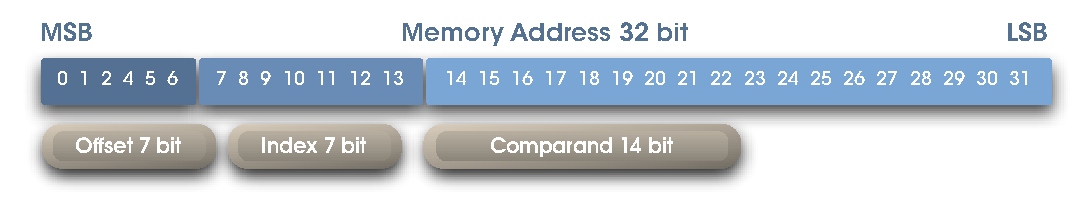
\includegraphics[width=\textwidth]{diagramme/addsplit_cache}
\caption{Address layout for the 4-Way Set Associative Cache}
\label{fig:4way_address_layout}
\end{figure}


\subsubsection{Cache Lookup}
For the cache lookup three SIMD vectors are needed. The first vector contains
four copies of the comparand, the second four copies of the index and the third
four copies of the offset.

To obtain the four copies of the comparand the desired address is bitwise-anded
with a splat of 0xFFFFFC00 (18 bits of the address) to populate the vector.
As only the valid entries are interesting for the lookup the result is bitwise-ored
with 0x00000001. The last bit is used for identifying if an entry is valid or not.
In that way the cache lookup routine will only consider valid entries.

The four copies of the index and offset are obtained in the same way as the
comparand but now with a splat of 0x00003F80 (7 bit index) respectively
0x0000007F (7 bit offset).

To clear the picture the figure \ref{fig:addr_splat} shows the resulting
vectors after applying the bit operation on the address 0x12345678.

\begin{figure}[H]
\centering
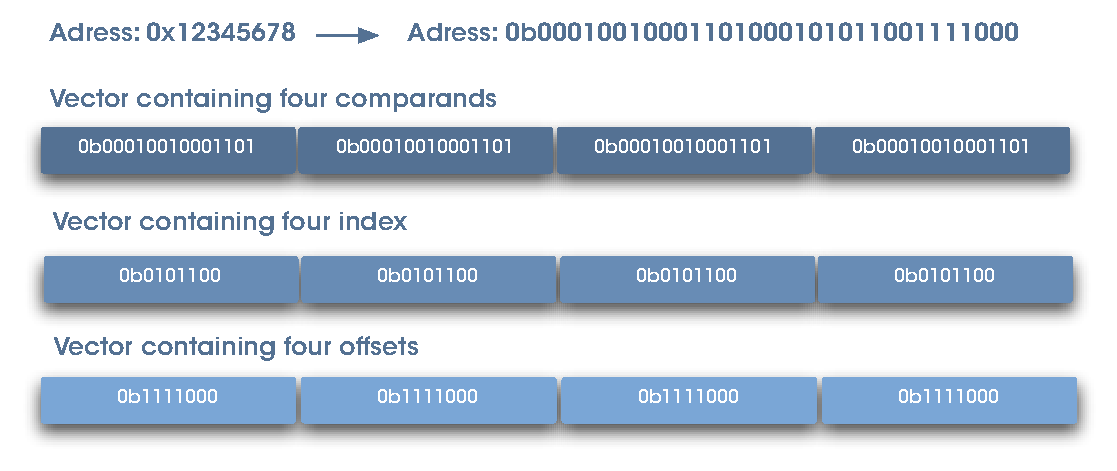
\includegraphics[width=\textwidth]{diagramme/addr_splat}
\caption{The three resulting vectors after applying the bit operations}
\label{fig:addr_splat}
\end{figure}


Adding the byte index into the tag and address array  yields the address of
the entries which might hold the desired cache line. The corresponding tag and
address entries are loaded into two SIMD vectors. The first contains four
comparands matching the tag array entry that is to be examined. The
second contains four addresses to cache lines.

The next step is to compare the comparands obtained from the address with the
comparands stored in the tag array. The comparison is done with the
\textit{spu\_cmpeq} intrinsic. Each element of the first vector is compared with
 the corresponding element of the second vector at the same time. If the operands
are equal, all bits of the corresponding element of the resulting vector are set
to one. If they are unequal, all bits of the corresponding element of the resulting
vector are set to zero.


If there is a match all the bits of one element of the resulting vector will be
set to one and the data in question is in the cache (cache hit) otherwise all
bits of the vector will be set to zero (cache miss).

Before the inspection can be done the information from the vector must be extracted.
Therefore the \textit{spu\_gather} intrinsic is used. It gathers all rightmost bits
(LSB) from each element and returns the bits in the rightmost bits of element 0 of the
returned vector.

This value can now be extracted with the \textit{spu\_extract} intrinsic and compared
to a scalar value.

\subsubsection{Cache Hit}
\label{sec:cacheh}
If the value is non-null there exists a tag in the cache that is equal to the tag
obtained from the address. The resulting vector of the tag comparison that can be seen
as a mask, is used to extract the corresponding address to the cache line. This is
simply done by a bitwise-anded operation between the mask and the address array entry.

Now the resulting vector is rotated so that the corresponding address is in the
preferred slot\footnote{The preferred slot is always element 0 of a vector}. After
adding the offset within the given cache line the address is ready to be returned.


\subsubsection{Cache Miss}
\label{sec:cachem}

The cache miss handler first of all looks for a free slot. The determination of the
free slot is similar to finding a matching tag. First of all a mask is created which
indicates which slot is free and which is occupied. With the \textit{spu\_gather}
intrinsic a value is extracted in which the state of the slots is encoded.

The figure \ref{fig:slot_state} shows the resulting value of two occupied
and two free slots.

\begin{figure}[H]
\centering
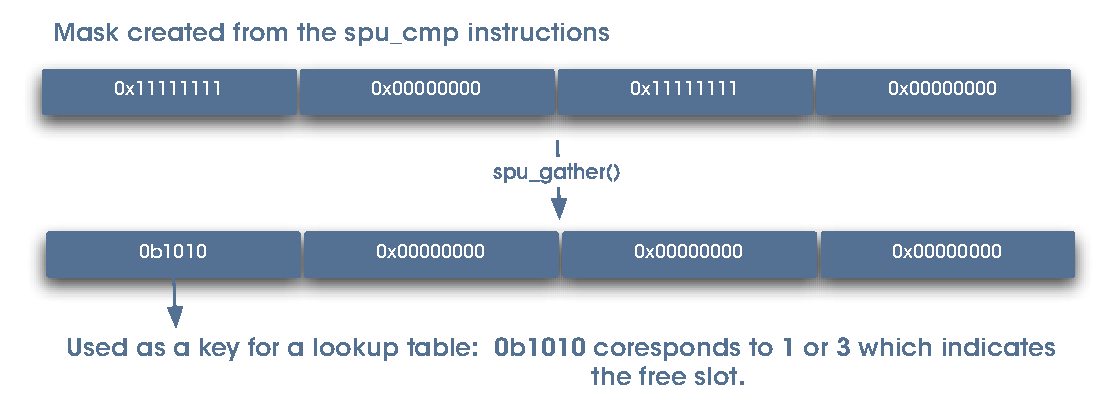
\includegraphics[width=\textwidth]{diagramme/slot_state}
\caption{The resulting value that represents the state of the set}
\label{fig:slot_state}
\end{figure}

This gathered value is a key for a lookup table which translates the value into
a value between 0-3 which indicates which slot is free. The lookup table is a
vector with 16 short ints. A preprocessing step involves the initalization of the
vector for correct mapping between the key and the corresponding value.

If the set is full a cache replacement policy is applied and a slot is randomly
freed. The free slot is returned and the cache miss handler can now fetch the desired cache line from main memory.

The address is always aligned to 128 byte boundaries since the cache only fetches
128 bytes to minimize the overhead. When the Memory Flow Controller (MFC) engine
 finishes fetching the data the corresponding comparands and address to this cache
 line is created and saved with valid bit set into the cache.

After adding the offset to the requested address the address can be returned.



\section{Load Balancer}
\label{sec:impl_load_balancer}
The main problem which arises when implementing a communication framework for the
Cell BE in the context of load balancing is that the SPEs do not know which device
has written to its MMIO register. Each SPE can \textit{talk} to any other SPE by signals
or mailboxes. It is a \textit{N:N} relationship, where N is the count of SPE involved.
Therefore it was fundamental to divide the event handling into two domains and to encode
an unique id into the signals respectively into the messages send from other SPEs.
At thread creation time each SPE an id is assigned to distinguish each SPE.

Now with the knowledge that the SPE has to deal with load balancing, as the signals
are recieved through the \textit{signal 2 notification} channel, the signals can be
decoded an the reciever always knows which SPE has send it a signal.

Each SPE has a lookup table where the handle to the MMIO register of any other SPE
is stored. With the extracted or any other id each SPE has the ability to send signals
or messages to a specific SPE. Why this differentiation is done will shown next.

A seen in the section \ref{sec:design_load_balancer} the system graph describes a chain
of nodes. The head of the chain the \textit{SPE 7} can only communicate with the
\textit{SPE 6}. But \textit{SPE 6} has also a handle to \textit{SPE 5} and so on.

If now \textit{SPE 7} gets out of work it looks up which nodes are connected to it and
sends a specific signal to the corresponding node which is \textit{SPE 6}. The
\textit{SPE 6} receives  the signal through the event handling system and calls
the loadbalancer.
The loadbalancer decodes the id which are the 3 LSB of the signal and calculates
the remaining workload. The \textit{SPE 6}  now waits until the \textit{SPE 7}
has sent their workload through the \textit{mailbox} channel. After receiving the
message both the \textit{SPE 7} and the \textit{SPE 6} calculate their workload
to exchange after the Generalized Dimension Exchange method. The message are as well
encoded to distinguish which SPE has send the workload.

The \textit{SPE 7} that has requested workload now enlarges the lower bound of the
tile and the \textit{SPE 6} reduces the higher bound of the tile.

It is clear that when the \textit{SPE 6} is requesting workload the higher bound
is modified according to the workload from \textit{SPE 7} as well as the lower
bound is modified according to the workload from \textit{SPE 5}.


\chapter{Results and Conclusion}

The main impact of the \textit{predecessor work} was the access to the main memory.
Features like prefetching or double-buffering weren't used at all. Furthermore
very few hardware characteristics were exploited.
The new application architecture tried to exploit the hardware characteristic
at a higher degree. The use of the shared memory model had advantages over
the other programming models. The data stayed on chip as long as possible, the
communication overhead was reduced and the PPE could be completely decoupled from
the load balancing and work assignment. Furthermore the SPEs were not dependent
on each other as the SPEs were autonomous ray tracers which could ray trace
the whole image or a tile. The use of shared memory programming model led to a rendering time improvement of a factor of 3.

The use of a cache in the application architecture was a remedial action to improve
overall performance. Beside other techniques for efficient use of variables stored
in main memory like prefetching and double buffering only the cache has the ability
to exploit locality of reference and reduce access to main memory. The overall
performance increased by an factor of 13.5.

Another improvement was the use of a load balancing scheme. In ray tracing or any
other rendering algorithm the tiling strategy is susceptible to load imbalance.
Experiments show that the overall performance could be further increased by a
factor of 2. It must be noted that these experiments were done for the simple
ray tracing algorithm. The situation may look different with Monte-Carlo Ray Tracing
or with global illumination.

\subsubsection*{Conclusion}

The Cell Broadband Engine is a very powerful processor with many superior features
compared to general-purpose processors in desktop machines. However there is huge
step to take in the development process to achieve good performance. There are not
only the consideration about the data flow. The developer has to choose a appropriate
programming model. He has to consider about the application partitioning and
which parts to offload to the SPE. Should the code be vectorized or the data access
patterns improved or both? This are some questions which arise during programming for
the Cell BE.

The essential thing is that the developer must be aware that the Cell BE is not
an conventional processor. The SPEs provide computational density advantage over
conventional processors through their programmability. The advanced instruction
set and supported data types of the SPEs facilitates the Cell BE to deal with a
wide variety of applications. The developer is not limited to a specific field
of computation but can develop applications for network processing, graphics,
cryptography of high performance computing.

Near theoretical maximum performance can be achieved for real applications on
the Cell BE processor unlike to conventional processors. The programmer musst be
aware and unterstand the architectural characteristics of the processor to achieve
optimal performance.


\bibliography{diplomarbeit}
 \printnomenclature
\end{document}
